\documentclass{report}
\usepackage{graphicx}
\newcommand{\Aprime}{A$'$}
\newcommand{\IL}{I_L}
\newcommand{\pendiente}[1]{\par\textbf{[PENDIENTE (requiere datos): #1]}\par}
\newcommand{\pend}[1]{\textbf{[#1]}}
\newcommand{\SI}[2]{#1~#2}
\newcommand{\si}[1]{#1}
\newcommand{\percent}{\%}
\newcommand{\celsius}{°C}
\newcommand{\mm}{mm}
\newcommand{\url}[1]{\texttt{#1}}
\newcommand{\glsaddall}{}
\newcommand{\thependcount}{21}
\newcommand{\Titulo}{Estimación morfométrica monocular de peces a través de una interfaz aire--vidrio--agua: comparación de modelos de calibración y cuantificación de la incertidumbre por profundidad desconocida}
\newcommand{\TituloMay}{ESTIMACIÓN MORFOMÉTRICA MONOCULAR DE PECES A TRAVÉS DE UNA INTERFAZ AIRE--VIDRIO--AGUA: COMPARACIÓN DE MODELOS DE CALIBRACIÓN Y CUANTIFICACIÓN DE LA INCERTIDUMBRE POR PROFUNDIDAD DESCONOCIDA}
\newcommand{\Autor}{Cipriano Ezequiel Pereira López}
\newcommand{\Tutora}{Ing. Evelyn Giménez}
\newcommand{\Directora}{Andrea Mercado Kroll}
\newcommand{\Universidad}{Universidad Católica Nuestra Señora de la Asunción}
\newcommand{\Campus}{Campus Guairá}
\newcommand{\Unidad}{Unidad Académica de Ciencias y Tecnología}
\newcommand{\Carrera}{Carrera de Ingeniería en Informática}
\newcommand{\Ciudad}{Villarrica}
\newcommand{\Fecha}{octubre de 2026}
\newcommand{\Anio}{2026}
\newcommand{\PalabrasClave}{morfometría de peces; visión monocular; refracción; calibración de cámara; puerto plano}
\newcommand{\Keywords}{fish morphometry; monocular vision; refraction; camera calibration; flat port}
\newcommand{\RepoURL}{https://github.com/Zequi20/FishmeterTPF}
\newcommand{\RepoTag}{v1.0-tesis}
\newcommand{\RepoCommit}{0d71b69a8a7757b118d5f421f1958a0ecbb09214}
\newcommand{\RepoCommitShort}{0d71b69}

\begin{document}
\title{\Titulo}\author{\Autor}\date{\Ciudad, \Fecha}\maketitle
\section*{Proyecto Final de Carrera}
PROYECTO FINAL DE CARRERA presentado como requisito para optar al título de Ingeniero en Informática, \Universidad, \Campus, \Unidad. Tutora: \Tutora. Directora: \Directora.

Palabras clave: \PalabrasClave.



{\large\bfseries PÁGINA DE ADVERTENCIA\par}

\vspace{1cm}
Por este medio, declaro que el presente documento titulado:

\emph{«\Titulo»}

es de mi autoría, excluyendo las citas, referencias y materiales de apoyo utilizados para contextualizar el tema investigado y los objetivos del estudio.

Asimismo, declaro que el trabajo no se ha presentado previamente bajo este título para la obtención de otro título profesional o académico equivalente.
\vspace{3cm}

\\ \Autor




\vspace*{5cm}


\emph{A mi familia, que durante estos años me esperó con la cena guardada y aprendió a no preguntar cuándo terminaba la tesis.}




\chapter*{Agradecimientos}
\addcontentsline{toc}{chapter}{Agradecimientos}
A mi tutora, por revisar cada versión del protocolo y devolverla con observaciones concretas. Le agradezco en especial que insistiera en separar lo que los datos permiten afirmar de lo que solo parecía razonable; volví a esa pregunta en cada capítulo.

A la Universidad Católica Nuestra Señora de la Asunción, Campus Guairá, y en particular a la Dirección de la Carrera y al plantel docente de la Unidad Académica de Ciencias y Tecnología, por la formación de estos años y por responder consultas que excedían el contenido de sus asignaturas. Usé lo aprendido en álgebra lineal, por ejemplo, en cada homografía y en cada calibración de este trabajo.

A mis compañeros de curso, por las horas de estudio compartidas y por escuchar, más de una vez, mi explicación de por qué un pez parece más grande dentro de una pecera.

A quienes me ayudaron con la impresión de las réplicas y con las primeras pruebas del montaje. Varias de esas pruebas salieron mal, y de ellas aprendí más que de las que funcionaron al primer intento.

A mi familia, por el apoyo económico y por la paciencia durante los meses en que ocupé la mesa del comedor con una pecera y una cámara sobre un trípode.


\chapter*{Resumen}
\addcontentsline{toc}{chapter}{Resumen}
La medición morfométrica de peces a partir de imágenes evita manipular al animal, pero cuando la cámara observa a través de la pared de un tanque la refracción en la interfaz aire--vidrio--agua modifica la escala aparente según la profundidad del pez, y una sola cámara no permite conocer esa profundidad. Este trabajo evaluó, en un montaje controlado, cuatro estrategias de conversión de píxeles a milímetros aplicadas a los mismos puntos anatómicos: una escala directa con un marcador ArUco fijo en el vidrio (A), una homografía con marcador coplanar (\Aprime), una calibración pinhole efectiva realizada bajo el agua (B) y un modelo refractivo explícito de puerto plano (C). Se utilizaron seis réplicas rígidas impresas en PLA medidas con calibre, cuatro profundidades (5, 11, 17 y 23 cm) y tres capturas por condición, con un total de 72 imágenes y 24 combinaciones réplica--profundidad. Los cuatro puntos se marcaron manualmente una vez por imagen y se reutilizaron en los cuatro métodos. Con la profundidad conocida, C obtuvo el menor error de longitud total (MAE \SI{1,22}{mm}; \SI{0,88}{\percent}), seguido de \Aprime{} (\SI{3,29}{mm}; \SI{2,28}{\percent}), B (\SI{16,32}{mm}; \SI{11,24}{\percent}) y A (\SI{37,43}{mm}; \SI{25,68}{\percent}), y fue el mejor en las seis réplicas y en las 24 combinaciones réplica--profundidad (prueba de signos por réplica, $p = 0{,}031$). El error de A creció de \SI{13,8}{} a \SI{57,6}{mm} al alejar la réplica del vidrio, en concordancia con la predicción geométrica de primer orden. Con la misma geometría, el intervalo de longitud inducido por una profundidad desconocida tiene un ancho de 56 a 83~\% de la longitud si la profundidad no se acota, y de 4 a 6~\% si se conoce con $\pm 1$~cm. Se concluye que, a través de un vidrio plano, el modelo refractivo reduce el error de conversión por debajo del 1~\% y que la profundidad, no la refracción, es la fuente dominante de incertidumbre cuando se desconoce. Los resultados se limitan al montaje, a las réplicas rígidas y a las condiciones ópticas utilizadas.

\noindent\textbf{Palabras clave:} \PalabrasClave.


\chapter*{Abstract}
\addcontentsline{toc}{chapter}{Abstract}

Image-based fish morphometry avoids handling the animal, but when the camera looks through the wall of a tank, refraction at the air--glass--water interface changes the apparent scale with the depth of the fish, and a single camera cannot recover that depth. This work evaluated, in a controlled setup, four strategies for converting pixels to millimetres applied to the same anatomical points: a direct scale from an ArUco marker fixed to the glass (A), a homography from a coplanar marker (\Aprime), an effective pinhole calibration performed under water (B), and an explicit flat-port refractive model (C). Six rigid PLA replicas measured with a calliper, four depths (5, 11, 17 and 23 cm) and three captures per condition were used, for a total of 72 images and 24 replica--depth combinations. The four points were marked manually once per image and reused by all four methods. With known depth, C achieved the lowest total-length error (MAE 1.22 mm; 0.88\,\%), followed by \Aprime{} (3.29 mm; 2.28\,\%), B (16.32 mm; 11.24\,\%) and A (37.43 mm; 25.68\,\%), and was the best method in all six replicas and all 24 replica--depth combinations (sign test by replica, $p = 0.031$). The error of A grew from 13.8 to 57.6 mm as the replica moved away from the glass, in agreement with a first-order geometric prediction. With the same geometry, the length interval induced by an unknown depth spans 56 to 83\,\% of the length when depth is unconstrained, and 4 to 6\,\% when depth is known to within $\pm 1$~cm. It is concluded that, through a flat glass, the refractive model reduces the conversion error below 1\,\% and that depth, rather than refraction, is the dominant source of uncertainty when it is unknown. The results are limited to the setup, the rigid replicas and the optical conditions used.

\noindent\textbf{Keywords:} \Keywords.



\chapter*{Lista de acrónimos}
\begin{description}
\item[3D] tridimensional
\item[CSV] valores separados por comas (\emph{comma-separated values})
\item[EA] error absoluto
\item[JPG] formato de imagen del Joint Photographic Experts Group
\item[JSON] JavaScript Object Notation
\item[LT] longitud total
\item[MAE] error absoluto medio
\item[MAPE] error porcentual absoluto medio
\item[MFLD-net] Mobile Fish Landmark Detection network
\item[OpenCV] Open Source Computer Vision Library
\item[PC] profundidad corporal
\item[PLA] ácido poliláctico (material de impresión 3D)
\item[RMS] raíz cuadrática media (\emph{root mean square})
\item[RMSE] raíz del error cuadrático medio
\item[YAML] YAML Ain't Markup Language
\end{description}
\chapter{Introducción y planteamiento del problema}

\section{Introducción}

La piscicultura requiere mediciones morfométricas para describir el crecimiento, estimar el rendimiento y apoyar la selección de ejemplares. Las mediciones manuales son informativas, pero demandan tiempo, personal capacitado y, cuando se trabaja con animales vivos, manipulación que puede producir estrés o lesiones \parencite{Fernandes2020,Saleh2023,Torres2018}. La visión por computadora ofrece una alternativa para obtener medidas a partir de imágenes, pero la detección correcta del pez no garantiza por sí sola una medida física correcta.

Cuando la fotografía se toma desde el aire a través de la pared de un tanque, la luz atraviesa agua, vidrio y aire y se desvía en cada cambio de medio. Una cámara que observa a través de una interfaz aire--vidrio--agua con puerto plano no se comporta, en general, como una cámara pinhole central \parencite{Agrawal2012,Treibitz2012}: la escala aparente del pez depende de su distancia al vidrio, y una sola cámara no permite conocer esa distancia. Una calibración pinhole realizada en el medio puede absorber parcialmente la refracción cerca de la distancia de calibración, pero el error cambia al alejar el objeto de esa zona \parencite{Rofallski2022}.

Este trabajo evaluó, en un montaje controlado, cuatro formas de convertir píxeles a milímetros aplicadas a los mismos puntos anatómicos de la misma imagen: una escala directa con un marcador ArUco fijo en el vidrio (A), una homografía con un marcador coplanar con la réplica (\Aprime), una calibración pinhole efectiva realizada bajo el agua (B) y un modelo refractivo explícito de puerto plano (C). Las unidades experimentales fueron réplicas rígidas de peces medidas con calibre, no peces vivos. Con la profundidad conocida se comparó el error de las cuatro rutas; con la profundidad desconocida se cuantificó, mediante C, el intervalo de longitud que inducen los límites físicos de la pecera, y se determinó cuánto debe acotarse la profundidad para que ese intervalo sea utilizable. La configuración conceptual de la cámara, el vidrio, el agua y los rayos refractados se muestra en la Figura~\ref{fig:1-1}.

\begin{figure}[htbp]
\centering
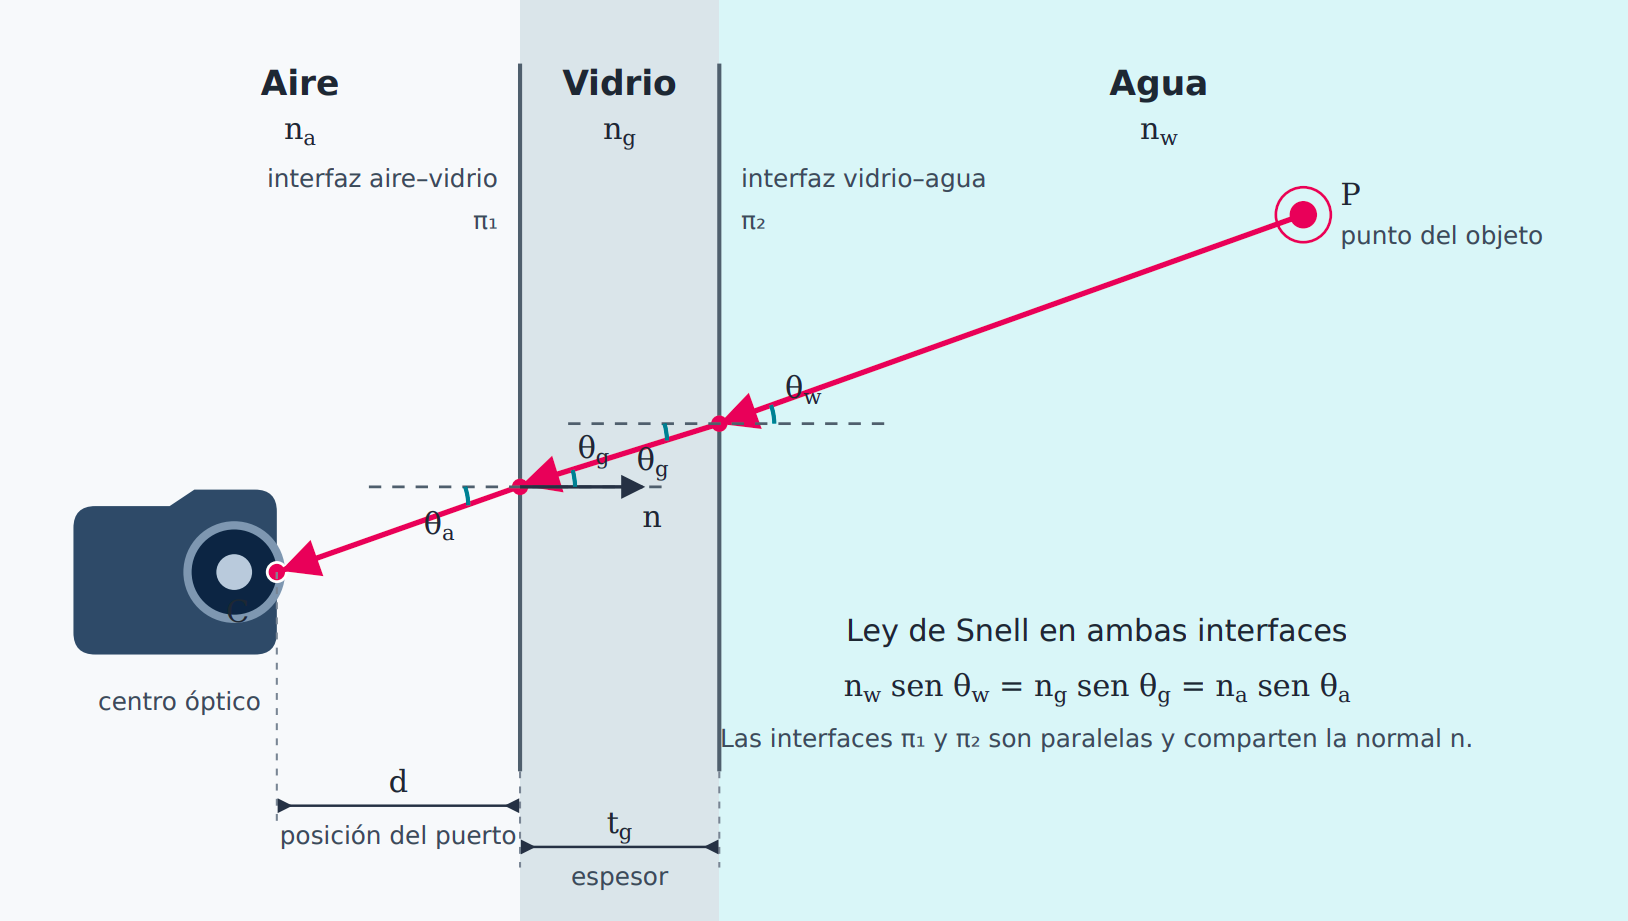
\includegraphics{figuras/originales/fig1_1_configuracion.png}
\caption[Configuración conceptual de cámara, vidrio, agua y rayos refractados]{Configuración conceptual de cámara, vidrio, agua y rayos refractados. El rayo que llega al sensor desde el punto $P$ se quiebra en las interfaces $\pi_1$ y $\pi_2$, de modo que el píxel «ve» el punto en un lugar distinto del que ocupa; el desplazamiento depende de la distancia $d$, del espesor $t_g$ y de la profundidad $z$ del punto detrás del vidrio. Fuente: elaboración propia.}
\label{fig:1-1}
\end{figure}

\section{Elección del tema}

El tema surgió de una necesidad práctica y de una observación simple: para medir un pez en una pecera con una cámara común hay que decidir cómo pasar de píxeles a milímetros, y las tres alternativas habituales (un marcador de escala, una calibración de cámara hecha bajo el agua o un modelo óptico explícito) dan respuestas distintas para la misma fotografía. La bibliografía demuestra que la refracción afecta la medición, pero no dice cuánto vale cada alternativa, sobre los mismos puntos y contra una referencia física, en la configuración más frecuente en un laboratorio o en una instalación pequeña: una cámara fuera de un vidrio plano.

Se estudió un flujo monocular de medición con marcado manual de puntos anatómicos sobre imágenes de réplicas rígidas fotografiadas a través de una pecera de vidrio. La conversión de píxeles a milímetros se comparó mediante cuatro rutas, A, \Aprime, B y C, aplicadas a los mismos puntos de cada imagen y evaluadas contra la medida física de cada réplica. El tema combina visión por computadora, geometría proyectiva y metrología; su aporte informático es un procedimiento de medición monocular con incertidumbre explícita por profundidad y un módulo de trazado refractivo implementado y verificado experimentalmente.

\section{Antecedentes}

Los trabajos previos muestran que los puntos anatómicos y una referencia de escala pueden extraerse de imágenes mediante procedimientos automáticos o manuales \parencite{Correia2025,Saleh2023,Tseng2020}. Los primeros enfoques trabajaron fuera del agua o en montajes controlados: \textcite{Monkman2019} detectaron el pez y un marcador ArUco situado junto al ejemplar y aproximadamente coplanar; \textcite{Fernandes2020} segmentaron imágenes de tilapia para extraer medidas corporales; y \textcite{Saleh2023} localizaron puntos anatómicos para realizar morfometría. Estos antecedentes respaldan la obtención de información morfométrica mediante imágenes, pero también muestran que la localización de puntos no equivale por sí sola a una medición física exacta, y ninguno resuelve la formación de la imagen a través de una pared de vidrio ni la variación de escala con la profundidad.

En ambientes acuáticos, además de localizar al pez, es necesario recuperar su escala o profundidad. \textcite{AlJubouri2017} emplearon dos cámaras ortogonales, mientras que \textcite{Zhou2023} y \textcite{Seibold2026} recurrieron a visión estéreo y triangulación. MorphoCal es monocular, pero la cámara está sumergida y los puntos se proyectan sobre un plano de referencia definido mediante una calibración pinhole realizada bajo el agua \parencite{Vijayalakshmi2026}. \textcite{Yin2026} corrigieron la refracción en una interfaz aire--agua y analizaron la sensibilidad frente a distintas profundidades asumidas, pero emplearon una profundidad nominal y no entregaron un intervalo de longitud. Pinax y CalibMar son antecedentes de modelos o herramientas para puertos planos, no sistemas de medición de peces \parencite{Luczynski2017,Seegraber2025}. En los trabajos revisados no se encontró una evaluación monocular que compare A, \Aprime, B y C sobre los mismos puntos y que, además, cuantifique el intervalo de longitud cuando la profundidad es desconocida. El estado del arte y la comparación detallada de estos enfoques se desarrollan en el Capítulo~\ref{cap:marco}.

\section{Planteamiento del problema}

La medición morfométrica a partir de imágenes puede reducir la manipulación y facilitar la repetición del seguimiento de peces. No obstante, en una escena que atraviesa la interfaz aire--vidrio--agua la proyección no es una cámara perspectiva simple. La refracción y la separación de profundidad entre el pez y el marcador de escala pueden producir una longitud aparente distinta de la longitud física, incluso cuando los cuatro puntos anatómicos estén bien marcados.

El problema metodológico consiste en separar tres fuentes que suelen quedar mezcladas: la escala directa de un marcador en el vidrio, la calibración aproximada de una cámara bajo el agua y el modelado explícito de los rayos a través de un puerto plano. Para ello se compararon, en la misma imagen y sobre los mismos puntos anatómicos, las rutas A, \Aprime, B y C. La ruta C se evaluó además para el rango de profundidades físicamente posibles. El resultado de esa evaluación no es un intervalo de confianza estadístico, sino el rango geométrico $[\min_{z} L(z), \max_{z} L(z)]$ inducido por desconocer $z$ dentro de $[z_{\min}, z_{\max}]$; la notación abreviada $[L(z_{\min}), L(z_{\max})]$ solo es válida si $L(z)$ es monótona en el intervalo considerado.

El estudio se restringió a réplicas rígidas observadas lateralmente, con la longitud total y la profundidad corporal como medidas principales; esta última se mide sobre el cuerpo y excluye las aletas. Los cuatro puntos anatómicos se marcaron manualmente una sola vez sobre la imagen original y se reutilizaron en las cuatro rutas. Las capturas adicionales de una réplica fueron repeticiones técnicas y no unidades experimentales independientes. Esta delimitación permitió aislar el efecto geométrico, pero impide generalizar directamente a peces vivos, movimiento, turbidez, oclusiones o posturas no laterales.

A partir de esta brecha y de la delimitación adoptada, la siguiente sección formula la pregunta principal y las preguntas secundarias que orientaron la investigación.

\section{Preguntas de investigación}

\paragraph{Pregunta principal.} ¿Qué intervalo de longitud puede garantizar C cuando $z$ es desconocida y en qué condiciones su ancho resulta utilizable para una medición morfométrica?

\paragraph{Preguntas secundarias.}
\begin{enumerate}
  \item Con $z$ conocida, ¿cómo se comportan A, \Aprime, B y C en longitud total y profundidad corporal (sin incluir aletas), y cómo cambia el error de A y de B al alejarse de la zona de calibración de B?
  \item ¿Qué repetibilidad presenta el marcado manual de los cuatro puntos anatómicos y cómo afecta a la estimación de las dos medidas?
  \item ¿Qué sensibilidad tiene la estimación de C a los parámetros geométricos del montaje medidos a mano (distancia cámara--vidrio e índice de refracción del agua)?
\end{enumerate}

\section{Objetivos}

\paragraph{Objetivo general.} Evaluar una cadena monocular de estimación morfométrica de peces a través de una interfaz aire--vidrio--agua, comparando cuatro estrategias de conversión métrica sobre los mismos puntos anatómicos y cuantificando el intervalo de longitud inducido por una profundidad desconocida mediante un modelo refractivo de puerto plano, con validación frente a referencias físicas de réplicas rígidas.

\paragraph{Objetivos específicos.}
\begin{enumerate}
  \item Construir y documentar el conjunto de datos de réplicas, referencias físicas, posiciones, distancias, repeticiones y exclusiones.
  \item Establecer un protocolo reproducible para marcar manualmente los cuatro puntos anatómicos y cuantificar la repetibilidad de ese marcado.
  \item Implementar y validar las rutas A, \Aprime, B y C, incluido el módulo C de puerto plano, frente a las referencias físicas de las réplicas.
  \item Comparar de forma pareada el error de longitud total y profundidad corporal sin aletas entre A, \Aprime, B y C según la separación de la zona de calibración de B.
  \item Calcular el intervalo $[\min_z L(z), \max_z L(z)]$ sobre el rango físicamente admisible de profundidad, junto con su ancho relativo y su cobertura.
  \item Evaluar la sensibilidad de las estimaciones a la repetibilidad del marcado manual y a las condiciones geométricas del montaje.
\end{enumerate}

La Tabla~\ref{tab:trazabilidad} relaciona cada objetivo específico con la pregunta que responde, la hipótesis asociada cuando corresponde, la sección donde se presenta el resultado y la conclusión que lo cierra.

\begin{table}[htbp]

\caption{Trazabilidad entre preguntas, objetivos, hipótesis, resultados y conclusiones.}
\label{tab:trazabilidad}
\begin{tabular}{@{}cp{4.6cm}cccc@{}}
\hline
Obj. & Qué produce & Pregunta & Hipótesis & Resultado & Conclusión \\
\hline
1 & Conjunto de datos documentado & --- & --- & §\ref{sec:conjunto} & §\ref{sec:conclusiones}, c.~1 \\
2 & Protocolo y repetibilidad del marcado & S2 & --- & §\ref{sec:repetibilidad} & §\ref{sec:conclusiones}, c.~2 \\
3 & Rutas A, \Aprime, B y C implementadas y validadas & S1 & H1 & §\ref{sec:calibraciones}, §\ref{sec:agregados} & §\ref{sec:conclusiones}, c.~3 \\
4 & Comparación pareada por separación & S1 & H1, H2 & §\ref{sec:profundidad}, §\ref{sec:contraste} & §\ref{sec:conclusiones}, c.~4 \\
5 & Intervalo $\IL$, ancho y cobertura & Principal & H3 & §\ref{sec:intervalo} & §\ref{sec:conclusiones}, c.~5 \\
6 & Sensibilidad a marcado y geometría & S2, S3 & --- & §\ref{sec:sensibilidad}, §\ref{sec:repetibilidad} & §\ref{sec:conclusiones}, c.~6 \\
\hline
\end{tabular}
\end{table}

\section{Justificación}

La obtención de medidas morfométricas repetibles puede apoyar el seguimiento del crecimiento, la estimación del rendimiento y la selección de ejemplares en acuicultura. Una cadena basada en imágenes puede disminuir la manipulación directa y hacer más frecuente la observación; en este proyecto esa motivación no se convirtió en una afirmación de desempeño en peces vivos, porque la validación se realizó con réplicas rígidas y en un montaje controlado. \pend{Si se dispone de una fuente verificada (MAG o FAO), incluir aquí una cifra de producción piscícola de Paraguay con su cita; de lo contrario, mantener la justificación técnica.}

La relevancia informática está en estudiar el límite métrico de un procedimiento monocular cuando la escena atraviesa un puerto plano. El trabajo mantuvo constantes la imagen y los cuatro puntos marcados manualmente, comparó A, \Aprime, B y C sobre las mismas observaciones e hizo explícita la salida de incertidumbre geométrica por profundidad. Así, el resultado no se reduce a una interfaz ni a una promesa de medición sin intervención humana: produce evidencia para decidir cuándo una escala directa es suficiente, cuándo conviene una calibración pinhole y cuándo es necesario un modelo refractivo.

La contribución comprende cinco componentes verificables: una salida monocular que explicita la incertidumbre atribuible a la profundidad; evidencia comparativa de A, \Aprime, B y C en un montaje controlado; una implementación propia del modelo de puerto plano basada en formulaciones publicadas y evaluada contra referencias físicas; un protocolo reproducible de marcado manual con réplicas rígidas; y un análisis de la repetibilidad de los puntos anatómicos. El informe comunica el error de cada ruta y el ancho relativo del intervalo $[\min_z L(z), \max_z L(z)]$ sobre el rango físicamente admisible. Dicho intervalo no cubre por sí solo errores de calibración, postura, marcado manual o referencia física; esas fuentes se midieron y reportaron por separado.

La extrapolación a peces vivos, turbidez, movimiento, oclusión o instalaciones productivas queda como limitación y trabajo futuro, no como una capacidad demostrada.

\section{Hipótesis y variables}

La unidad experimental es cada réplica rígida de pez. Una captura adicional de la misma réplica es una repetición técnica y no se considera una unidad independiente. Los criterios de decisión de cada hipótesis se fijaron en términos de las cantidades que efectivamente se calcularon en el Capítulo~\ref{cap:resultados}.

\subsection{Hipótesis de investigación}

\begin{description}
  \item[H1 --- Comparación geométrica con profundidad conocida.] Con la profundidad conocida, el error absoluto de longitud total de C es menor que el de A, \Aprime{} y B. Criterio: prueba de signos exacta sobre las diferencias pareadas por réplica ($n = 6$, unidad experimental), con $p < 0{,}05$; el conteo por combinación réplica--profundidad se reporta como descriptivo. La equivalencia entre B y C dentro de la zona de calibración de B, prevista en el protocolo con un margen $\delta$, no se evaluó formalmente porque el margen no se fijó antes de observar los datos; se informa la diferencia observada.
  \item[H2 --- Dependencia con la distancia.] La diferencia $\mathrm{error}(B) - \mathrm{error}(C)$ aumenta con la separación respecto de la zona de calibración de B. Criterio: pendiente positiva de la diferencia de MAE de longitud total frente a la separación (0, 6, 12 y 18~cm).
  \item[H3 --- Intervalo por profundidad desconocida.] El intervalo calculado con C,
  \begin{equation*}
    \IL = \Big[\min_{z} L(z),\ \max_{z} L(z)\Big],
  \end{equation*}
  contiene la longitud física de la réplica cuando $z$ recorre el rango físicamente admisible, y su ancho relativo es predecible a partir de la geometría del montaje ($d$, $t_g$, índices y rango de $z$). Criterio: cobertura empírica objetivo $\geq 0{,}95$ sobre las capturas disponibles y diferencia entre el ancho predicho y el observado menor que la mitad del ancho. Su ancho relativo se reporta como predicción geométrica, no como intervalo de confianza.
\end{description}

\subsection{Variables}

\begin{description}
  \item[Independientes.] Método (A, \Aprime, B, C); distancia de la réplica al vidrio y separación respecto de la zona de calibración de B; rango de $z$ usado para el intervalo.
  \item[Dependientes.] Error con signo, error absoluto y porcentual de longitud total y profundidad corporal, excluyendo aletas; ancho relativo y cobertura del intervalo.
  \item[Controladas.] Cámara y sus ajustes, pecera, agua, iluminación, marcadores, soporte, protocolo de marcado manual, operador y unidades experimentales.
\end{description}

La definición conceptual y operacional de cada variable se presenta en la Tabla~\ref{tab:operacionalizacion} del Capítulo~\ref{cap:metodologia}.

\section{Alcance y limitaciones del diseño}

El aporte defendible es una evaluación comparativa del instrumento, acompañada de una caracterización de la incertidumbre geométrica por profundidad desconocida. La investigación no promete un sistema listo para operar en instalaciones productivas: sus resultados quedan acotados por las réplicas rígidas, la cámara monocular, el rango de índices de refracción, la postura lateral y las condiciones controladas documentadas en la metodología.

Entre las limitaciones se consideraron la selección manual de los puntos, la repetibilidad del operador y su posible efecto sobre las medidas anatómicas. Estas fuentes de variación se documentaron en el dominio de la pecera. El flujo no se describe como automático: la selección anatómica siempre requirió marcado manual.

\subsection{Delimitación espacial y temporal}

El experimento se realizó en \Ciudad, Paraguay, en un montaje de laboratorio doméstico. Las capturas definitivas y las calibraciones de cámara se realizaron el 12 de octubre de 2026, según consta en los perfiles de calibración (Anexo~\ref{anx:calibraciones}). La revisión bibliográfica tuvo como fecha de corte septiembre de 2026. \pend{Completar el mes de inicio del montaje y de las primeras pruebas.}

\section{Estructura del documento}

El documento se organiza en cinco capítulos.

\begin{description}
  \item[Capítulo I. Introducción y planteamiento del problema.] Presenta la motivación, los antecedentes breves, la brecha, las preguntas, los objetivos, la justificación, las hipótesis, las variables, el alcance, las limitaciones y la estructura.
  \item[Capítulo II. Marco teórico y estado del arte.] Desarrolla la morfometría, la formación de imágenes en una interfaz plana, las rutas A, \Aprime, B y C, el marcado manual de puntos, los marcadores ArUco, la evaluación de mediciones y la síntesis de antecedentes.
  \item[Capítulo III. Metodología.] Describe el diseño pareado, la población y la muestra, el montaje, los instrumentos, las calibraciones, la captura, el procesamiento de las imágenes, el análisis y la trazabilidad del experimento.
  \item[Capítulo IV. Resultados y discusión.] Organiza los datos y exclusiones, las calibraciones, la comparación A, \Aprime, B y C, el comportamiento según la profundidad, el intervalo por profundidad desconocida, el contraste de hipótesis y la discusión.
  \item[Capítulo V. Conclusiones y recomendaciones.] Presenta la regla de decisión que resume el aporte, una conclusión por objetivo, las limitaciones reales, las recomendaciones, el trabajo futuro y el impacto potencial separado de lo demostrado.
\end{description}

Los anexos conservan el registro visual de las capturas, los parámetros del puerto plano, los perfiles de calibración, la referencia geométrica del riel, el índice del repositorio y el registro de cambios de esta versión.

\chapter{Marco teórico y estado del arte}
\label{cap:marco}

En este capítulo se desarrollan los conceptos que permiten comprender la estimación morfométrica a partir de imágenes obtenidas en un medio acuático controlado. El proceso comprende la definición de las medidas físicas de referencia, la formación de la imagen a través de la interfaz aire--vidrio--agua, el marcado manual de puntos anatómicos, la recuperación de la escala física y la comparación de las estimaciones con los valores de referencia. La organización conceptual de estos componentes se resume en la Figura~\ref{fig:2-1}.

\begin{figure}[htbp]
\centering
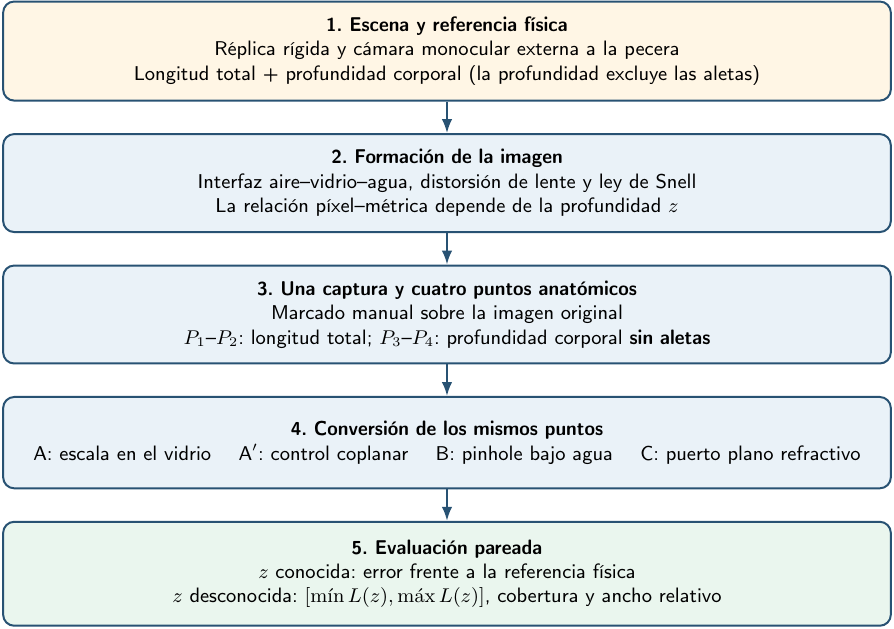
\includegraphics{figuras/originales/fig2_1_flujo.png}
\caption[Flujo teórico simplificado de la investigación]{Flujo teórico simplificado de la investigación: escena y referencia física, formación refractiva de la imagen, marcado manual único de puntos, comparación de las rutas A, \Aprime, B y C y evaluación con profundidad conocida o desconocida. Fuente: elaboración propia.}
\label{fig:2-1}
\end{figure}

\section{Medición morfométrica de peces}

\subsection{Morfometría y parámetros corporales}

La morfometría comprende la medición de características externas relacionadas con el tamaño y la forma de los organismos. En peces, estas medidas pueden obtenerse mediante instrumentos manuales o mediante el análisis digital de imágenes, y resultan útiles para describir variaciones corporales y obtener datos biométricos \parencite{Petrtyl2014}.

Para esta investigación se consideran únicamente dos medidas principales: longitud total y profundidad corporal. La reducción no es una omisión accidental: el marcado manual permite localizar sus extremos geométricos, pero no identifica de forma inequívoca la placa hipural ni el margen posterior del opérculo necesarios para la longitud estándar y la longitud cefálica. La profundidad corporal sí es una salida principal y se define de forma estricta para que no se confunda con una dimensión que incluya aletas.

La longitud total representa el tamaño general y se obtiene entre el extremo anterior del hocico y el extremo posterior de la aleta caudal. La profundidad corporal se obtiene entre los perfiles dorsal y ventral del cuerpo, en la sección donde la separación es máxima, excluyendo por completo las aletas dorsal, ventral, pectorales y caudal. En otras palabras, las aletas pueden intervenir en la longitud total cuando forman parte del extremo caudal, pero nunca se incorporan a la profundidad corporal. Ambas medidas mantienen exactamente los mismos puntos en la referencia física y en A, \Aprime, B y C. Esta decisión evita seleccionar después la medida que resulte más favorable.

\subsection{Puntos anatómicos y definición de las medidas}
\label{sec:puntos-def}

La medición morfométrica lineal requiere establecer puntos anatómicos de referencia reproducibles. Aunque algunas denominaciones, en particular la longitud estándar, no siempre se aplican de manera uniforme en la literatura, en este trabajo se adoptan las siguientes definiciones \parencite{Howe2002,Saleh2023,Steeds2024}:

\begin{description}
  \item[Longitud total (LT):] distancia desde el punto más anterior del hocico hasta el punto más posterior de la aleta caudal, correspondiente al extremo del radio caudal de mayor longitud. Operacionalmente, en este trabajo se mide como la proyección del segmento entre ambos puntos sobre el eje longitudinal del cuerpo (ecuación~\ref{eq:medidas}); cuando los puntos están sobre el eje, coincide con la distancia euclídea.
  \item[Profundidad corporal (PC):] mayor distancia dorsoventral entre los perfiles dorsal y ventral del cuerpo, medida en la sección de separación máxima y excluyendo las aletas. Los extremos de esta medida se ubican sobre el perfil del cuerpo, no sobre la punta de una aleta.
\end{description}

Estas definiciones establecen las referencias anatómicas que se conservan tanto en la medición física como en la estimación obtenida desde las imágenes. La longitud estándar y la longitud cefálica quedan como antecedentes o trabajo futuro, no como variables del protocolo principal, porque sus puntos no son observables inequívocamente con los cuatro puntos definidos para el marcado manual. Las definiciones de los puntos y medidas se ilustran en la Figura~\ref{fig:2-2}.

\begin{figure}[htbp]
\centering
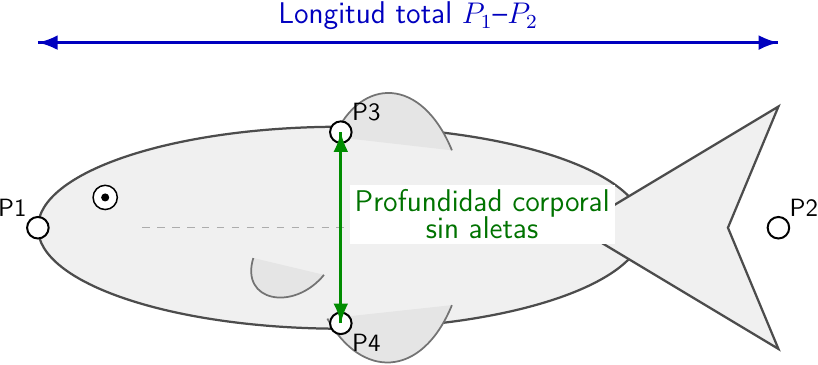
\includegraphics{figuras/originales/fig2_2_puntos.png}
\caption[Puntos anatómicos y medidas morfométricas consideradas]{Puntos anatómicos y medidas morfométricas consideradas. La longitud total incluye el extremo caudal; la profundidad corporal se mide solo sobre el cuerpo y excluye las aletas. Fuente: elaboración propia.}
\label{fig:2-2}
\end{figure}

Las mediciones realizadas directamente sobre los modelos físicos se utilizan como valores de referencia para evaluar las estimaciones obtenidas desde las imágenes. Sin embargo, estas mediciones no deben considerarse valores completamente exentos de error, puesto que pueden verse afectadas por la resolución del instrumento, la identificación de los puntos anatómicos y la repetibilidad del procedimiento. Por ello, la comparación mantiene las mismas definiciones anatómicas en la medición física y en la estimación digital.

\subsection{Exactitud, repetibilidad e incertidumbre de la referencia}

La medición manual presenta variabilidad interobservador e intraobservador por diferencias en la localización de los puntos anatómicos, la presión aplicada, la posición del objeto, la resolución del instrumento y la experiencia de quien mide \parencite{Petrtyl2014}. Por ello, el valor manual no debe tratarse como una magnitud libre de incertidumbre, sino como una referencia obtenida mediante un procedimiento controlado.

La exactitud de la referencia expresa su proximidad al valor atribuible al mensurando, mientras que la repetibilidad describe la dispersión de lecturas realizadas bajo las mismas condiciones. La resolución y la exactitud declaradas del instrumento, la variación entre repeticiones y la selección de los puntos anatómicos contribuyen a la incertidumbre de la referencia. Esta incertidumbre debe considerarse al interpretar diferencias pequeñas entre el valor manual y el estimado.

\section{Formación de imágenes en medios acuáticos}

\subsection{Modelo geométrico convencional de cámara}

El modelo de cámara estenopeica o \emph{pinhole} representa la formación de la imagen como una proyección perspectiva en la que los rayos provenientes de la escena atraviesan un único centro de proyección antes de alcanzar el plano de la imagen. Bajo este modelo, la relación entre un punto tridimensional expresado en el sistema de coordenadas del mundo y su proyección sobre la imagen puede escribirse como \parencite{Hartley2004,Zhang2000}:
\begin{equation}
\lambda \begin{bmatrix} u \\ v \\ 1 \end{bmatrix} = \mathbf{K}\,[\mathbf{R} \mid \mathbf{t}]\begin{bmatrix} X_w \\ Y_w \\ Z_w \\ 1 \end{bmatrix},
\label{eq:pinhole}
\end{equation}
donde $(X_w, Y_w, Z_w)$ son las coordenadas del punto en el sistema de referencia del mundo, $(u, v)$ son sus coordenadas en la imagen y $\lambda$ es un factor de escala asociado con la profundidad del punto.

La matriz $\mathbf{K}$ reúne los parámetros intrínsecos de la cámara:
\begin{equation}
\mathbf{K} = \begin{bmatrix} f_x & \gamma & c_x \\ 0 & f_y & c_y \\ 0 & 0 & 1 \end{bmatrix},
\label{eq:K}
\end{equation}
donde $f_x$ y $f_y$ corresponden a las distancias focales expresadas en píxeles, $(c_x, c_y)$ representa el punto principal y $\gamma$ describe la posible falta de perpendicularidad entre los ejes del sensor. Estos parámetros caracterizan la transformación desde las coordenadas de la cámara hasta las coordenadas de la imagen y, en principio, no dependen de la posición de la cámara en la escena \parencite{Hartley2004}.

Los parámetros extrínsecos están representados por la matriz de rotación $\mathbf{R}$ y el vector de traslación $\mathbf{t}$. En conjunto, definen la transformación rígida desde el sistema de coordenadas del mundo hacia el sistema de coordenadas de la cámara y, por tanto, establecen su pose respecto de la escena \parencite{Hartley2004,Zhang2000}.

El modelo pinhole constituye una aproximación ideal y no incluye por sí mismo la distorsión introducida por la lente. En una cámara convencional, esta aproximación suele complementarse con coeficientes de distorsión radial y tangencial. Sin embargo, cuando la adquisición se realiza a través de interfaces aire--vidrio--agua, la refracción modifica adicionalmente la dirección de los rayos y puede invalidar el supuesto de un único centro de proyección \parencite{Treibitz2012,Seegraber2025}.

\subsection{Distorsión óptica producida por la lente}

El modelo pinhole supone que la cámara produce una proyección perspectiva ideal. Sin embargo, una lente real puede introducir desplazamientos geométricos que modifican la posición observada de los puntos en la imagen. Una formulación convencional representa estos desplazamientos mediante componentes radiales y tangenciales \parencite{Brown1966,Weng1992}.

Sean $(x, y)$ las coordenadas normalizadas que tendría un punto bajo una proyección ideal y sea
\begin{equation}
r^2 = x^2 + y^2,
\end{equation}
donde $r$ representa la distancia del punto al eje óptico en el plano normalizado. Las coordenadas afectadas por la distorsión, denotadas por $(x_d, y_d)$, pueden expresarse como
\begin{equation}
\begin{aligned}
x_d &= x\left(1 + k_1 r^2 + k_2 r^4 + k_3 r^6\right) + 2p_1 xy + p_2\left(r^2 + 2x^2\right),\\
y_d &= y\left(1 + k_1 r^2 + k_2 r^4 + k_3 r^6\right) + p_1\left(r^2 + 2y^2\right) + 2p_2 xy.
\end{aligned}
\label{eq:distorsion}
\end{equation}

Los coeficientes $k_1$, $k_2$ y $k_3$ representan la componente radial. Su efecto depende de la distancia $r$ y generalmente se vuelve más apreciable hacia los bordes de la imagen, donde puede producir patrones de distorsión de barril o de cojín. Los coeficientes $p_1$ y $p_2$ representan la componente tangencial o por descentrado, asociada principalmente con la falta de alineación entre los elementos de la lente, el eje óptico y el sensor. Por ello, esta componente puede producir desplazamientos asimétricos en diferentes regiones de la imagen.

Estos coeficientes describen desviaciones pertenecientes al sistema cámara--lente. En una calibración convencional se estiman junto con los parámetros intrínsecos de la cámara mediante la minimización del error de reproyección, bajo el supuesto de una cámara central o pinhole \parencite{Zhang2000}. La compensación obtenida permite aproximar la proyección que produciría una cámara ideal sin distorsión de lente.

La refracción producida por un puerto plano constituye un fenómeno diferente. Cuando los rayos atraviesan las interfaces aire--vidrio--agua, sus trayectorias dejan de ajustarse, en general, a un único centro de proyección. El sistema puede describirse entonces como una cámara axial no central, cuya geometría depende de la orientación y posición de las interfaces, sus espesores y los índices de refracción de los medios \parencite{Agrawal2012,JordtSedlazeck2012}.

\subsection{Refracción en la interfaz aire--vidrio--agua}

La refracción ocurre cuando un rayo de luz atraviesa medios con índices de refracción diferentes. Para una interfaz entre dos medios, la ley de Snell relaciona el ángulo de incidencia $\theta_1$, el ángulo refractado $\theta_2$ y los índices de refracción $n_1$ y $n_2$ \parencite{Hecht2017}:
\begin{equation}
n_1 \sin\theta_1 = n_2 \sin\theta_2 .
\label{eq:snell}
\end{equation}

Los ángulos se miden respecto de la normal de la interfaz. En la configuración del proyecto, la luz procedente del objeto atraviesa sucesivamente el agua, la pared transparente y el aire situado delante del sistema óptico; en la retroproyección desde la cámara, el orden es aire, vidrio y agua. La ley de Snell debe aplicarse en cada interfaz considerando los índices de refracción, la orientación de las superficies y su geometría. Según \textcite{Seegraber2025}, la refracción ocasionada por una carcasa o un puerto altera el modelo de formación de la imagen: la trayectoria de los rayos depende de la forma y orientación del puerto, de la posición de la cámara respecto de este y de las propiedades de los medios atravesados.

\subsection{Modelo refractivo de puerto plano}
\label{sec:puerto-plano}

Un puerto plano puede representarse mediante dos interfaces paralelas: una entre el aire y la pared transparente, y otra entre esta pared y el agua. Para describir la trayectoria asociada a un píxel resulta conveniente considerar la retroproyección desde la cámara hacia la escena. Debido al principio de reversibilidad óptica, esta trayectoria coincide, en sentido contrario, con la recorrida por la luz desde el objeto hasta la cámara \parencite{Agrawal2012,JordtSedlazeck2012}. La geometría del puerto plano considerada se representa en la Figura~\ref{fig:2-3}.

\begin{figure}[htbp]
\centering
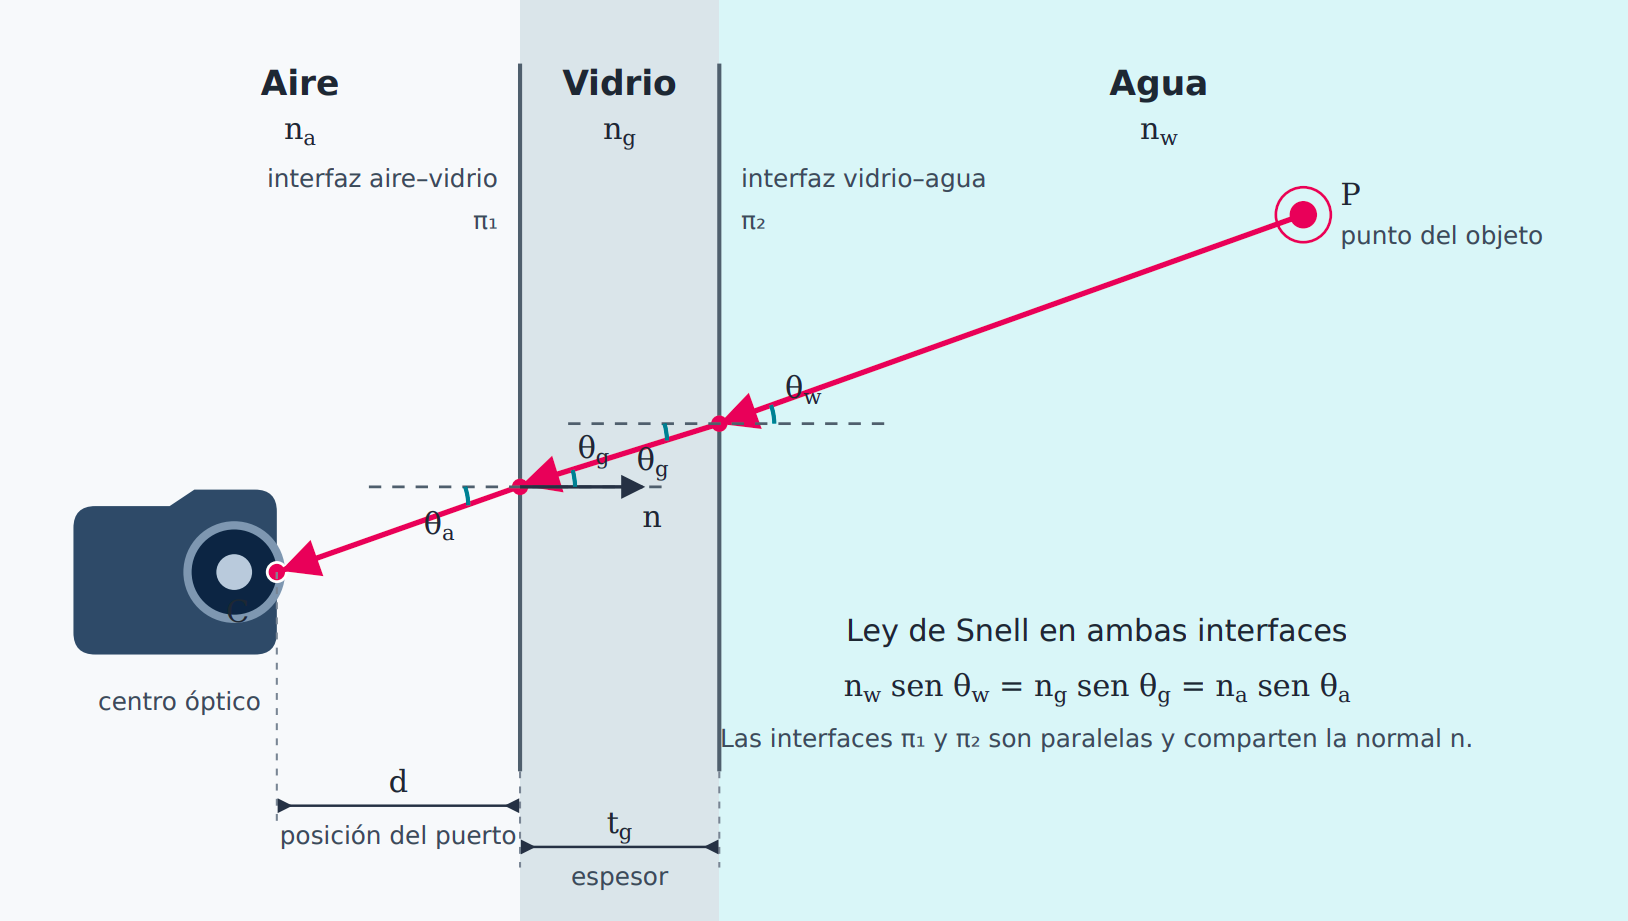
\includegraphics{figuras/originales/fig2_3_puerto_plano.png}
\caption[Modelo refractivo de puerto plano]{Modelo refractivo de puerto plano: centro de cámara $C$, interfaces $\Pi_1$ (aire--vidrio) y $\Pi_2$ (vidrio--agua) a distancias $d$ y $d + t_g$ del centro, normal común $\mathbf{n}_\pi$, puntos de intersección $\mathbf{q}_1$ y $\mathbf{q}_2$ y direcciones $\mathbf{v}_a$, $\mathbf{v}_g$ y $\mathbf{v}_w$ en aire, vidrio y agua. Fuente: elaboración propia a partir de \textcite{Agrawal2012}.}
\label{fig:2-3}
\end{figure}

Sea el centro de proyección de la cámara el origen del sistema de coordenadas y sea $\mathbf{n}_\pi$ un vector unitario normal a las interfaces, orientado desde la cámara hacia la escena. La cara exterior de la pared transparente (del lado del aire, $\Pi_1$) y su cara interior (del lado del agua, $\Pi_2$) pueden expresarse como
\begin{align}
\Pi_1 &: \mathbf{n}_\pi^{\mathsf{T}}\mathbf{X} = d, \label{eq:pi1}\\
\Pi_2 &: \mathbf{n}_\pi^{\mathsf{T}}\mathbf{X} = d + t_g, \label{eq:pi2}
\end{align}
donde $d$ es la distancia perpendicular entre el centro de cámara y la primera interfaz, mientras que $t_g$ representa el espesor de la pared. Esta representación supone que las dos superficies son planas, paralelas y poseen la misma normal.

Para un punto de imagen homogéneo $\tilde{\mathbf{p}} = (u, v, 1)^{\mathsf{T}}$, previamente corregido de la distorsión propia de la lente, la dirección unitaria del rayo en aire se obtiene mediante
\begin{equation}
\mathbf{v}_a = \frac{\mathbf{K}^{-1}\tilde{\mathbf{p}}}{\lVert \mathbf{K}^{-1}\tilde{\mathbf{p}} \rVert},
\label{eq:va}
\end{equation}
donde $\mathbf{K}$ es la matriz de parámetros intrínsecos de la cámara. El primer punto de intersección del rayo con la cara exterior del puerto es
\begin{equation}
\mathbf{q}_1 = \frac{d}{\mathbf{n}_\pi^{\mathsf{T}}\mathbf{v}_a}\,\mathbf{v}_a .
\label{eq:q1}
\end{equation}

La dirección refractada al pasar de un medio $i$ a un medio $j$ puede representarse mediante la forma vectorial de la ley de Snell. Si $\mathbf{v}_i$ es una dirección unitaria incidente y $\eta_{ij} = \mu_i/\mu_j$ es la razón entre los índices de refracción, entonces
\begin{equation}
\mathcal{R}(\mathbf{v}_i; \mu_i, \mu_j, \mathbf{n}_\pi) = \eta_{ij}\left(\mathbf{v}_i - (\mathbf{v}_i^{\mathsf{T}}\mathbf{n}_\pi)\,\mathbf{n}_\pi\right) + \sqrt{1 - \eta_{ij}^2\left(1 - (\mathbf{v}_i^{\mathsf{T}}\mathbf{n}_\pi)^2\right)}\;\mathbf{n}_\pi .
\label{eq:snell-vec}
\end{equation}

De este modo, la dirección del rayo dentro de la pared transparente queda determinada por
\begin{equation}
\mathbf{v}_g = \mathcal{R}(\mathbf{v}_a; \mu_a, \mu_g, \mathbf{n}_\pi),
\label{eq:vg}
\end{equation}
donde $\mu_a$ y $\mu_g$ son los índices de refracción del aire y del material de la pared, respectivamente. El rayo recorre entonces el espesor $t_g$ hasta intersectar la segunda interfaz. El punto de salida del vidrio se obtiene como
\begin{equation}
\mathbf{q}_2 = \mathbf{q}_1 + \frac{t_g}{\mathbf{n}_\pi^{\mathsf{T}}\mathbf{v}_g}\,\mathbf{v}_g .
\label{eq:q2}
\end{equation}

Al aplicar nuevamente la ley de Snell en la interfaz vidrio--agua se obtiene la dirección final del rayo en el agua:
\begin{equation}
\mathbf{v}_w = \mathcal{R}(\mathbf{v}_g; \mu_g, \mu_w, \mathbf{n}_\pi),
\label{eq:vw}
\end{equation}
donde $\mu_w$ es el índice de refracción del agua. Por tanto, el conjunto de puntos de la escena que pueden corresponder al píxel considerado queda representado por el rayo
\begin{equation}
\mathbf{X}(\lambda) = \mathbf{q}_2 + \lambda\,\mathbf{v}_w, \qquad \lambda \geq 0 .
\label{eq:rayo}
\end{equation}
Equivalentemente, un punto tridimensional $\mathbf{X}$ compatible con la observación debe satisfacer la restricción
\begin{equation}
(\mathbf{X} - \mathbf{q}_2) \times \mathbf{v}_w = \mathbf{0}.
\label{eq:restriccion}
\end{equation}

La normal $\mathbf{n}_\pi$ determina tanto la orientación de las interfaces como los ángulos de incidencia empleados en cada aplicación de la ley de Snell. Cuando la normal coincide con el eje óptico, el efecto refractivo presenta una disposición aproximadamente simétrica respecto del centro de la imagen. Una desalineación entre ambos modifica de manera distinta los rayos según su posición en la imagen y elimina dicha simetría.

La distancia $d$ establece la posición de la primera interfaz respecto del centro de cámara y, por tanto, determina el punto $\mathbf{q}_1$ donde el rayo abandona el aire. Esta distancia no modifica por sí sola el ángulo impuesto por la ley de Snell, pero sí desplaza los puntos de intersección y la posición espacial del rayo resultante. De forma similar, el espesor $t_g$ determina la distancia recorrida dentro de la pared y el desplazamiento entre $\mathbf{q}_1$ y $\mathbf{q}_2$.

Los índices $\mu_a$, $\mu_g$ y $\mu_w$ intervienen mediante sus razones y determinan el cambio de dirección en cada interfaz. En el caso de dos superficies paralelas, el ángulo final del rayo respecto de la normal depende de los índices de los medios inicial y final; sin embargo, el índice del vidrio y su espesor continúan influyendo en el desplazamiento lateral y en el punto desde el cual el rayo se propaga dentro del agua.

Como cada píxel queda asociado con un punto de origen $\mathbf{q}_2$ y una dirección $\mathbf{v}_w$ diferentes, los rayos en el agua no convergen necesariamente en un único centro de proyección. La geometría de un sistema con interfaces planas y paralelas corresponde, en general, a una cámara axial no central: la trayectoria completa de cada rayo permanece en el plano formado por el rayo incidente y la normal del puerto \parencite{Agrawal2012}.

\paragraph{Aproximación de primer orden.} Para incidencia cercana a la normal, la ecuación~\eqref{eq:snell-vec} se linealiza y el sistema se comporta como una cámara pinhole cuya distancia efectiva al plano del objeto es
\begin{equation}
D(z) = d + \frac{t_g}{\mu_g} + \frac{z}{\mu_w},
\label{eq:Dz}
\end{equation}
donde $z$ es la profundidad del objeto detrás de la cara interior del vidrio. La magnificación de un objeto a profundidad $z$ resulta proporcional a $1/D(z)$. Esta relación no reemplaza al trazado completo, pero permite predecir el signo y el orden de magnitud del error de una escala tomada en el vidrio y el ancho del intervalo inducido por una profundidad desconocida; ambas predicciones se contrastan con los datos en el Capítulo~\ref{cap:resultados}.

\subsection{Profundidad, inclinación y acortamiento aparente}

La obtención de medidas físicas a partir de una imagen depende de la configuración geométrica entre la cámara, la interfaz transparente, el objeto observado y la referencia métrica. En una adquisición mediante una pared plana, la posición y el tamaño aparente del objeto pueden variar con su profundidad y su ubicación dentro del campo de visión.

Para que una medida observada represente adecuadamente las dimensiones del objeto, su plano lateral debe mantenerse aproximadamente paralelo al plano de la pared transparente. Una desviación fuera de este plano produce un acortamiento aparente de las dimensiones proyectadas. De manera similar, la inclinación del eje longitudinal modifica la orientación de la medida en la imagen y puede afectar la identificación de los puntos anatómicos.

La relación entre píxeles y unidades físicas obtenida mediante una referencia visual solo puede aplicarse directamente al objeto cuando ambos se encuentran bajo condiciones geométricas equivalentes. Una diferencia de profundidad entre el marcador y el modelo produce escalas aparentes distintas por efecto de la perspectiva y de la refracción, como ilustra la Figura~\ref{fig:2-5}.

\begin{figure}[htbp]
\centering
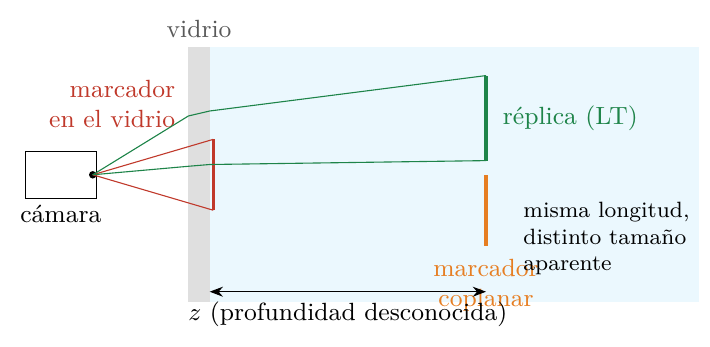
\includegraphics[width=\textwidth]{figuras/tikz/tikz_1.png}
\caption[Escala aparente de un marcador según su profundidad]{Un marcador fijo en el vidrio y una réplica situada a profundidad $z$ se observan con magnificaciones distintas: la escala del marcador (rojo) no se transfiere a la réplica (verde). Un marcador coplanar con la réplica (naranja) comparte su magnificación. Fuente: elaboración propia.}
\label{fig:2-5}
\end{figure}

La ubicación de la cámara, las dimensiones y el material del tanque, las distancias de trabajo, la posición del marcador y las tolerancias admitidas para la postura, la inclinación y la diferencia de profundidad constituyen decisiones del diseño experimental. Estos valores y el esquema del montaje se presentan en el Capítulo~\ref{cap:metodologia}.

\subsection{Profundidad conocida y profundidad desconocida}
\label{sec:z-desconocida}

La profundidad $z$ representa la distancia entre el objeto observado y la referencia geométrica fijada para el montaje, expresada respecto de la cara interna del vidrio o del sistema de coordenadas adoptado durante la calibración. Se considera conocida cuando la posición de la réplica se mide y controla mediante un soporte. En esa condición, los rayos pueden intersectarse con el plano correspondiente al objeto para producir una estimación puntual y comparar A, \Aprime, B y C frente a la referencia física.

La profundidad se considera desconocida cuando una imagen monocular no permite determinar de forma inequívoca la distancia del pez al vidrio. En tal caso, C se evalúa para el rango físicamente posible $z \in [z_{\min}, z_{\max}]$. Si $L(z)$ es la longitud estimada al asumir la profundidad $z$, el intervalo geométrico se define como
\begin{equation}
\IL = \Big[\min_{z \in [z_{\min}, z_{\max}]} L(z),\ \max_{z \in [z_{\min}, z_{\max}]} L(z)\Big].
\label{eq:IL}
\end{equation}

La forma abreviada $[L(z_{\min}), L(z_{\max})]$ solo es equivalente si se demuestra que $L(z)$ es monótona en el rango. En la aproximación de primer orden de la ecuación~\eqref{eq:Dz}, $L(z)$ es proporcional a $D(z)$ y, por tanto, creciente en $z$; la verificación numérica con el trazado completo se trata en el Capítulo~\ref{cap:resultados}. El intervalo propaga únicamente la profundidad desconocida: no cubre automáticamente incertidumbre de calibración, postura, marcado manual o referencia física, y no debe denominarse intervalo de confianza.

\subsection{Calibración y corrección refractiva}

El software CalibMar, desarrollado por \textcite{Seegraber2025}, permite calibrar cámaras y configuraciones de carcasa con puertos planos o en cúpula, estimando parámetros intrínsecos y parámetros asociados con la geometría refractiva. En este trabajo CalibMar es un antecedente instrumental: los perfiles de calibración se obtuvieron con la rutina \texttt{calibrateCamera} de OpenCV \parencite{Zhang2000} y la ruta C utiliza el trazado de rayos implementado en la aplicación propia (Sección~\ref{sec:metodos}).

El efecto geométrico se evalúa mediante las cuatro rutas A, \Aprime, B y C aplicadas a la misma escena. Mantener constantes la imagen, el criterio de marcado manual, los puntos anatómicos y la referencia física permite atribuir con mayor claridad las diferencias de error al tratamiento geométrico evaluado. En particular, la salida de una herramienta de calibración no se denomina automáticamente «corrección refractiva» ni se transforma sin verificación en coeficientes de distorsión de lente: C requiere parámetros, unidades, sistema de coordenadas y una implementación de trazado coherente con la geometría del montaje. En el experimento se documentan los parámetros consumidos por C, sus unidades y el sistema de coordenadas empleado.

\section{Estrategias de conversión métrica A, \Aprime, B y C}
\label{sec:rutas}

La comparación experimental se organiza en cuatro rutas geométricas aplicadas a los mismos puntos de cada imagen. La Figura~\ref{fig:2-4} las presenta lado a lado.

\begin{figure}[htbp]
\centering
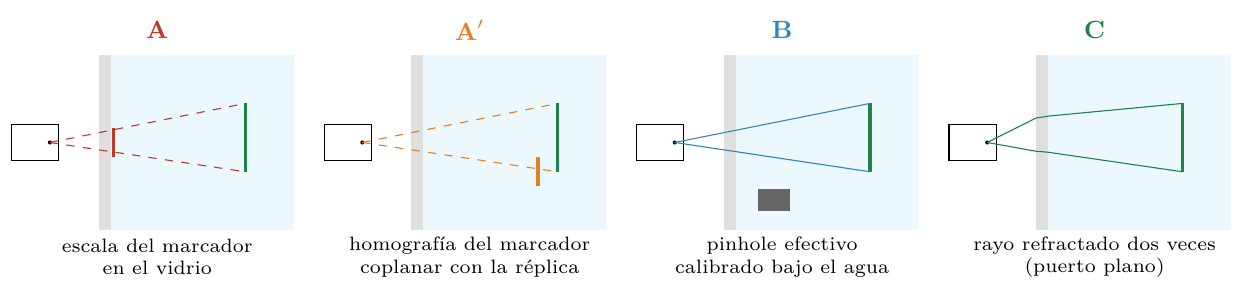
\includegraphics[width=\textwidth]{figuras/tikz/tikz_2.png}
\caption[Las cuatro rutas de conversión métrica lado a lado]{Las cuatro rutas de conversión métrica sobre la misma escena. A toma la escala de un marcador en el vidrio y supone rayos rectos; \Aprime{} rectifica el plano del marcador coplanar con la réplica; B usa una cámara pinhole con parámetros efectivos ajustados bajo el agua; C traza cada rayo a través de aire, vidrio y agua. Fuente: elaboración propia.}
\label{fig:2-4}
\end{figure}

\begin{description}
  \item[A: escala directa en el vidrio.] El marcador ArUco permanece en la pared de referencia y su dimensión conocida convierte píxeles a unidades físicas. La ruta es una línea base realista, pero sufre paralaje y escalas aparentes distintas si la réplica está a otra profundidad.
  \item[\Aprime: escala aproximadamente coplanar.] El marcador se coloca en el mismo plano de profundidad de la réplica, dentro de la tolerancia documentada en la metodología. Esta ruta controla cuánto del error de A proviene de la separación marcador--objeto. Como la rectificación se realiza por homografía, la diferencia entre A y \Aprime{} incluye tanto la coplanaridad como la corrección de perspectiva del plano del marcador.
  \item[B: cámara pinhole calibrada bajo el agua.] La calibración absorbe parte del efecto refractivo cerca de su zona de calibración; en este trabajo la calibración se realizó en la posición más cercana al vidrio y el error se estudió según la separación respecto de esa zona. La ruta B puede interpretarse como una compensación implícita de la refracción. Al calibrar un modelo pinhole con un patrón observado a través del mismo sistema aire--vidrio--agua, el procedimiento ajusta parámetros intrínsecos y coeficientes de distorsión efectivos para minimizar el error de reproyección en la zona cubierta por las imágenes de calibración. Aunque esta parametrización no reproduce la geometría no central de un puerto plano, puede aproximarla satisfactoriamente cuando las mediciones se realizan en un intervalo de distancias próximo al utilizado durante la calibración \parencite{JordtSedlazeck2012,Treibitz2012,Shortis2015}. La compensación necesaria depende, sin embargo, de la distancia entre la cámara y el punto observado, por lo que un único conjunto de parámetros pinhole no describe con igual exactitud objetos situados a diferentes profundidades. Las simulaciones de \textcite{Rofallski2022} muestran que la calibración implícita alcanza su mejor comportamiento cerca de la distancia de calibración y pierde exactitud al alejarse de ella, con una degradación adicional cuando el eje óptico y la interfaz no son perpendiculares. Este comportamiento fundamenta H2.
  \item[C: puerto plano explícito.] Se trazan los rayos a través de la interfaz aplicando la ley de Snell y las dimensiones se recuperan para una profundidad asumida. Al evaluar una grilla admisible de $z$ se obtiene $L(z)$ y, si $z$ es desconocida, el intervalo geométrico $[\min_z L(z), \max_z L(z)]$. C no aísla «la refracción» como única causa: incorpora el modelo completo de interfaces y la información de profundidad, y esa atribución se mantiene al interpretar sus resultados.
\end{description}

El marcado manual, la imagen y la referencia física permanecen constantes entre rutas. Por tanto, una diferencia entre métodos no debe atribuirse a una nueva selección anatómica ni a una imagen rectificada. El intervalo por profundidad no incorpora automáticamente incertidumbres de lente, calibración, postura, marcado manual o referencia; esas contribuciones se documentan por separado en el protocolo de repetibilidad y en la comparación geométrica.

\section{Marcado manual de puntos anatómicos}

En este proyecto no se utiliza una red ni un detector anatómico automático. Los cuatro puntos de cada captura se marcaron manualmente sobre la imagen original siguiendo una regla anatómica fija: $\mathbf{p}_1$ y $\mathbf{p}_2$ corresponden a los extremos de la longitud total, mientras que $\mathbf{p}_3$ y $\mathbf{p}_4$ corresponden a los extremos de la profundidad corporal, sin incluir ninguna aleta.

El marcado se realizó una sola vez por captura y las mismas coordenadas se reutilizaron en A, \Aprime, B y C. La identificación de la réplica, la imagen, el operador, la fecha, el criterio aplicado y cualquier revisión quedaron asociados al registro de medición. Una repetición de marcado o una revisión independiente permite estimar la repetibilidad del procedimiento, pero no se interpreta como una salida automática ni como una nueva unidad experimental.

La incertidumbre asociada con la localización manual se separó de la incertidumbre geométrica por profundidad. En particular, se documentaron los casos en que el contorno, la postura o la visibilidad de una aleta dificultaron ubicar un punto, y se conservó el motivo de cualquier exclusión. Esta separación permite atribuir las diferencias entre A, \Aprime, B y C al tratamiento geométrico sin cambiar los puntos anatómicos entre métodos.

\section{Recuperación de la escala física}

\subsection{Marcadores fiduciales ArUco}

Los marcadores ArUco son patrones fiduciales cuadrados compuestos por un borde negro y una matriz binaria interna que permite identificar cada marcador. Su detección proporciona el identificador y las coordenadas de sus cuatro esquinas en la imagen. Cuando se conoce el tamaño físico del marcador, estas esquinas constituyen correspondencias entre la imagen y una referencia del entorno \parencite{GarridoJurado2014}.

La información proporcionada por el marcador puede utilizarse de diferentes maneras. En una escena frontal y aproximadamente planar, su tamaño aparente permite establecer una relación local entre píxeles y unidades físicas. Si se conocen los parámetros intrínsecos y de distorsión de la cámara, también puede estimarse la pose del marcador respecto de esta. Por otra parte, las correspondencias entre las cuatro esquinas y sus posiciones conocidas en el plano permiten construir una homografía para rectificar dicho plano. Estas alternativas no son equivalentes: la escala directa supone una magnificación aproximadamente uniforme, la estimación de pose depende del modelo de cámara y la homografía solo representa correctamente los puntos pertenecientes al mismo plano.

El diccionario, el identificador, el tamaño físico, la alternativa de cálculo seleccionada y las reglas para aceptar o rechazar una detección son parámetros del sistema y se documentan en el Capítulo~\ref{cap:metodologia}.

\subsection{Conversión entre píxeles y unidades físicas}

En una escena frontal y aproximadamente planar, la dimensión física conocida del marcador puede utilizarse para obtener una escala local. Sea $L_m$ la longitud física de su lado y sean $p_i$, con $i = 1, \ldots, 4$, las longitudes en píxeles de los cuatro lados detectados. Cada longitud se calcula a partir de dos esquinas consecutivas:
\begin{equation}
p_i = \sqrt{(x_{i+1} - x_i)^2 + (y_{i+1} - y_i)^2},
\label{eq:lado}
\end{equation}
donde, para cerrar el contorno del marcador, se considera $(x_5, y_5) = (x_1, y_1)$.

\textcite{Monkman2019} estiman la longitud física representada por un píxel mediante el promedio de las escalas obtenidas de los cuatro lados del marcador:
\begin{equation}
k = \frac{1}{4}\sum_{i=1}^{4}\frac{L_m}{p_i},
\label{eq:escala-monkman}
\end{equation}
donde $k$ queda expresado en unidades físicas por píxel, por ejemplo, mm/píxel. El promedio de los cuatro lados reduce la dependencia de una única detección y permite considerar las pequeñas diferencias entre sus longitudes observadas en la imagen. La variante implementada en este trabajo, que divide el lado físico por el promedio de los cuatro lados en píxeles, se presenta en la Sección~\ref{sec:metodos}; ambas difieren en menos de una centésima de píxel para marcadores bien detectados.

Si $d_f$ representa la distancia en píxeles entre dos puntos anatómicos, la longitud física estimada se obtiene mediante
\begin{equation}
\hat{L}_f = k\,d_f .
\label{eq:Lf}
\end{equation}

Este procedimiento fue aplicado por \textcite{Monkman2019} para estimar la longitud total de peces utilizando marcadores ArUco de dimensiones conocidas. No obstante, la conversión supone que la magnificación puede considerarse uniforme entre el marcador y la región medida. Por ello, ambos deben encontrarse aproximadamente en el mismo plano y con una orientación equivalente respecto de la cámara. Una diferencia de profundidad introduce una variación de escala que la relación anterior no compensa.

Asimismo, las esquinas del marcador y los puntos anatómicos marcados deben expresarse en el mismo sistema de coordenadas y corresponder a la misma condición de corrección de la imagen. La etapa del procesamiento en la que se obtiene la escala y los criterios utilizados para revisar el marcado se especifican en el Capítulo~\ref{cap:metodologia}.

\subsection{Homografía, perspectiva y pose}

Una homografía rectifica únicamente el plano que la define. No recupera la posición tridimensional de puntos situados fuera de ese plano ni elimina la diferencia de escala producida por una separación de profundidad entre el marcador y el pez. Bajo refracción, además, la homografía constituye una aproximación del modelo físico: puede ajustar las correspondencias del plano de referencia, pero no representa necesariamente la trayectoria de todos los rayos aire--vidrio--agua. La formulación de la homografía utilizada por \Aprime{} se presenta en la Sección~\ref{sec:metodos}.

\section{Estimación y evaluación morfométrica}

La evaluación morfométrica debe separar tres propiedades. La exactitud describe la proximidad de una estimación a la referencia física; la repetibilidad describe la dispersión de repeticiones técnicas bajo las mismas condiciones; y la concordancia determina si dos procedimientos producen valores intercambiables, no solo si están correlacionados \parencite{Bland1986,Lin1989}. En este trabajo estas propiedades se examinaron sobre las mismas réplicas mediante errores con signo y absolutos, métricas agregadas y análisis pareados.

La referencia manual se trató como una medición controlada que también puede contener incertidumbre. Por ello, MAE, RMSE y MAPE se interpretan como diferencias respecto de esa referencia, mientras que el sesgo permite identificar una tendencia sistemática. Las repeticiones de una misma réplica se consolidaron antes de las comparaciones inferenciales; no constituyen unidades experimentales independientes. Las definiciones, fórmulas, agregaciones y criterios de decisión se presentan en el Capítulo~\ref{cap:metodologia}.

\subsection{Trazabilidad de la medición}

Además del valor estimado, un resultado reproducible debe identificar la imagen de origen, el modo de corrección, el perfil de calibración, el marcador empleado, el protocolo de marcado manual, el operador, la unidad y las advertencias de calidad. Esta información permite reconstruir la cadena desde la captura hasta la comparación con la referencia y distinguir los errores de adquisición, corrección, marcado y conversión métrica.

El contrato mínimo de salida, la estructura del archivo JSON y los artefactos que el procedimiento conserva para inspeccionar cada medición son decisiones de diseño e implementación. Su definición corresponde al Capítulo~\ref{cap:metodologia}, donde se describe la trazabilidad efectiva entre los datos de entrada, los resultados y las evidencias generadas.

\section{Antecedentes y trabajos relacionados}
\label{sec:antecedentes}

Se realizó una revisión narrativa estructurada de trabajos relacionados con medición morfométrica mediante imágenes, marcado manual o localización de puntos anatómicos, recuperación de escala y formación de imágenes a través de medios refractivos. La búsqueda inicial empleó términos como «fish measurement», «morphometric analysis», «fish size estimation», «non-invasive measurement» e «image processing». Posteriormente se incorporaron combinaciones más específicas, entre ellas «underwater fish length measurement», «fiducial marker fish measurement», «ArUco fish length», «flat-port camera», «air-glass-water refraction», «refractive camera calibration» y «refraction-aware fish measurement». La consulta se efectuó en Semantic Scholar y Google Scholar y se complementó mediante el seguimiento de referencias y la revisión de las fuentes originales. Debido a que no se estableció un protocolo exhaustivo de selección y exclusión, el procedimiento se considera una revisión narrativa y no una revisión sistemática. La búsqueda tuvo como fecha de corte septiembre de 2026. Se consideraron trabajos publicados en español o inglés que trataran al menos uno de los siguientes aspectos: medición morfométrica de peces mediante imágenes, recuperación de escala o puntos anatómicos, calibración de cámaras a través de interfaces aire--vidrio--agua, o modelos explícitos de refracción aplicables a una configuración acuática. Se excluyeron trabajos sin relación con mediciones de organismos acuáticos, calibración óptica, marcado de puntos o estimación de escala, así como duplicados y documentos que no permitieran identificar su fuente primaria. \pend{Indicar el número aproximado de resultados examinados y el número de trabajos seleccionados; en esta versión la Tabla~\ref{tab:antecedentes} incluye doce.}

Un primer grupo de antecedentes se relaciona con la obtención y evaluación de las medidas de referencia. \textcite{Petrtyl2014} compararon mediciones efectuadas con calibrador digital y mediante análisis de imágenes de carpa prusiana. El estudio incluyó 18 caracteres morfométricos, dos investigadores y comparaciones intraobservador e interobservador. Los sesgos relativos medios variaron entre $-4{,}27$~\% y $9{,}48$~\%, y se encontraron diferencias significativas en varias de las comparaciones. Estos resultados muestran que la medición manual y la digital pueden presentar tanto sesgo como variabilidad entre repeticiones y observadores. Por ello, el valor manual utilizado como referencia en este proyecto se obtuvo mediante un procedimiento controlado y no se trata como una magnitud libre de incertidumbre.

En cuanto a la automatización de la información anatómica, \textcite{Petrellis2021} combinó procesamiento de imágenes, detección de contornos, correspondencia de patrones y métodos de aprendizaje profundo para estimar longitud, profundidad corporal y área relativas, además de localizar aletas y otras regiones de interés. El error informado para la longitud varió entre 1,9~\% y 13,2~\%; sin embargo, el método trabajó principalmente con dimensiones relativas y planteó la visión estéreo como una extensión para recuperar dimensiones absolutas en peces inclinados u ocluidos.

\textcite{Saleh2023} propusieron MFLD-net, una red ligera para detectar 16 puntos anatómicos sobre imágenes de peces. A partir de estos puntos obtuvieron la longitud total, la longitud estándar, la longitud cefálica y la profundidad corporal. El modelo alcanzó una precisión promedio de detección $\mathrm{AP} = 0{,}967$ y errores absolutos medios de 9,25~mm para la longitud total, 8,27~mm para la longitud estándar, 6,57~mm para la longitud cefálica y 7,62~mm para la profundidad corporal. Este antecedente es especialmente relevante para la definición de los extremos anatómicos, aunque su montaje con cámara industrial y cinta transportadora no reproduce una adquisición a través de una pared aire--vidrio--agua.

En este proyecto, la localización anatómica se realizó mediante marcado manual. Este procedimiento evita atribuir a un procedimiento automático una precisión que no se evaluó y permite mantener exactamente los mismos cuatro puntos al comparar las rutas geométricas. La repetibilidad del marcado y la incertidumbre de la referencia física se documentan junto con las calibraciones.

Un segundo grupo de trabajos estudia la recuperación de escala. Mediante tres redes regionales, \textcite{Monkman2019} detectaron simultáneamente un pez y un marcador ArUco de tamaño conocido. La longitud total se calculó a partir del lado mayor de la región detectada y del promedio de las escalas correspondientes a los cuatro lados del marcador. El estudio informó una intersección sobre la unión media próxima al 93~\% y un sesgo porcentual medio de 2,2~\%. También identificó como fuentes principales de error la separación de profundidad entre el marcador y el pez, la distorsión de lente y las orientaciones absolutas superiores a aproximadamente $20^{\circ}$. Este antecedente fundamenta el uso de ArUco, pero también evidencia que el marcador solo proporciona una escala válida cuando se controlan la coplanaridad y la orientación.

De forma semejante, \textcite{Tseng2020} detectaron mediante una red convolucional las regiones de la cabeza, la horquilla caudal y una placa de color de dimensión conocida. Los puntos del hocico y de la horquilla se determinaron posteriormente mediante procesamiento de imágenes y la longitud se obtuvo utilizando la relación píxel--distancia de la placa. El clasificador alcanzó una exactitud del 98,78~\%, mientras que la longitud presentó un error absoluto medio de 5,36~cm y un error relativo absoluto medio de 4,26~\%. La diferencia entre estas cifras muestra que un desempeño elevado en detección no implica necesariamente una exactitud equivalente en la medición física.

En un tanque de producción, \textcite{Correia2025} utilizaron una cámara conectada a una Raspberry Pi y un modelo YOLOv8m-seg para segmentar camarones y una placa de alimentación de dimensiones conocidas. La placa se empleó como referencia de escala, mientras que la segmentación permitió seleccionar individuos extendidos y aproximadamente coplanares. Se obtuvieron valores de MAPE de 1,56~\% para la longitud y 0,15~\% para la anchura. Aunque el trabajo integra captura acuática, segmentación y escala visual, no formula una corrección refractiva explícita y estudia un objeto y una geometría diferentes de los considerados en esta investigación.

Los sistemas estéreo ofrecen otra forma de recuperar dimensiones físicas. \textcite{Marrable2023} combinaron detección profunda de cabeza y cola con un sistema estéreo BRUVS calibrado mediante estructuras tridimensionales. La comparación de 3954 mediciones automáticas y manuales produjo un coeficiente de correlación de Pearson de $r = 0{,}99$. Este resultado muestra una asociación lineal elevada, aunque la correlación no constituye por sí sola una medida de concordancia ni descarta la existencia de sesgo entre métodos. \textcite{AlJubouri2017} midieron la longitud de peces cebra a través de un tanque de vidrio con dos cámaras web ortogonales, despreciando el efecto del vidrio y compensando la distancia con la segunda vista.

Por su parte, \textcite{ZhangX2025} emplearon cámaras superior y lateral, una red basada en módulos Hourglass y transformaciones tridimensionales para obtener siete variables fenotípicas de bagre de canal dentro del agua. El error relativo medio fue de aproximadamente 3,7~\% para la longitud total y de 9,6~\% al considerar conjuntamente las siete variables. El trabajo demuestra la posibilidad de recuperar múltiples medidas en un montaje acuático, aunque no evalúa de forma separada el efecto de una corrección refractiva.

Los antecedentes específicamente ópticos cumplen una función diferente. \textcite{Qiao2019} propusieron un método de estructura a partir del movimiento que incorpora un modelo refractivo para estimar la calibración, la pose de la cámara y la reconstrucción tridimensional a través de superficies refractivas. El trabajo demostró, mediante simulaciones e imágenes reales, que ignorar la refracción introduce deformaciones en la reconstrucción. No obstante, su propósito es la reconstrucción tridimensional de escenas y no la medición morfométrica de peces.

En la calibración fotogramétrica de interfaces planas, el modelo Pinax de \textcite{Luczynski2017} representa de forma explícita la refracción en una carcasa de puerto plano y permite corregir la trayectoria de los rayos antes de realizar la reconstrucción o la medición. Este antecedente es conceptualmente cercano a la ruta C, aunque fue formulado para una corrección óptica general y no para comparar, en una misma captura monocular, una escala sin corrección, una calibración implícita y un modelo refractivo explícito. En la misma línea, \textcite{Rofallski2022} analizaron la distorsión dependiente de la distancia que aparece al aplicar modelos de cámara convencionales a interfaces multimedia planas, y \textcite{Shortis2015} revisó las técnicas de calibración para medición subacuática. Sus resultados respaldan que la compensación implícita depende de la profundidad y que la calidad de la calibración no puede resumirse en un único valor independiente de la zona de trabajo.

Tres antecedentes recientes delimitan con precisión la brecha. MorphoCal \parencite{Vijayalakshmi2026} es monocular, pero la cámara está sumergida y los puntos se proyectan sobre un plano de calibración fijo obtenido con un damero bajo el agua; informa un MAE de 0,75~cm y un RMSE de 0,86~cm sobre 4810 muestras. \textcite{Yin2026} corrigieron la refracción en la superficie agua--aire mediante la ley de Snell asumiendo una profundidad nominal (aproximadamente 0,8~m) y analizaron la sensibilidad a ese supuesto, sin entregar un intervalo. \textcite{Zhou2023} resolvieron la profundidad con visión estéreo y corrección de refracción en la superficie. Ninguno de los tres trata una cámara externa a un vidrio plano ni compara, sobre los mismos puntos, una escala directa, una calibración implícita y un modelo explícito.

\textcite{Seegraber2025} desarrollaron CalibMar, una herramienta abierta que integra la calibración de cámara, estéreo y carcasa para configuraciones con puertos planos o en cúpula. Para un puerto plano, el modelo estima parámetros relacionados con la orientación y posición de la interfaz y permite representar la trayectoria no central de los rayos. Este trabajo es un antecedente instrumental, pero no incorpora marcado anatómico, referencia ArUco ni evaluación de medidas de peces.

El antecedente de mayor proximidad óptica es el de \textcite{Seibold2026}, quienes estimaron la longitud de pequeños peces de agua dulce en acuarios mediante una cámara estéreo. Su método combina YOLOv11-Pose, correspondencias restringidas por geometría epipolar refractiva y triangulación tridimensional que considera explícitamente las interfaces aire--vidrio--agua. Los mejores resultados reportados alcanzaron RMSE de 6,11~mm y 9,22~mm en dos escenas de prueba. Este trabajo confirma la importancia de incorporar la refracción en la cadena de medición, aunque utiliza visión estéreo, no emplea un marcador ArUco y no compara, sobre las mismas observaciones, los resultados de una cadena con y sin corrección.

La Tabla~\ref{tab:antecedentes} resume las diferencias entre los antecedentes. Los valores numéricos no deben utilizarse para construir una clasificación directa entre métodos, debido a las diferencias de especie, tamaño, geometría, medidas, conjunto de datos y definición de las métricas.



\begin{longtable}{@{}p{2.2cm}p{2.8cm}p{2.6cm}p{3.0cm}p{3.0cm}p{3.2cm}p{3.6cm}@{}}
\caption{Matriz comparativa de antecedentes relacionados con la medición morfométrica y la corrección refractiva.}
\label{tab:antecedentes}\\
\hline
Fuente & Objeto y medio & Geometría & Puntos o procedimiento & Escala y refracción & Medidas y resultados & Limitación frente a este trabajo \\
\hline
\endfirsthead
\multicolumn{7}{l}{\small Tabla~\ref{tab:antecedentes} (continuación)}\\
\hline
Fuente & Objeto y medio & Geometría & Puntos o procedimiento & Escala y refracción & Medidas y resultados & Limitación frente a este trabajo \\
\hline
\endhead
\hline
\endfoot
\endlastfoot
\textcite{Monkman2019} & Lubina europea; fotografías fuera del agua & Monocular; tres cámaras no especializadas & R-CNN para pez y marcador; longitud por región envolvente & ArUco de lado conocido; solo distorsión de lente & LT; mIoU $\approx$ 93~\%; sesgo porcentual medio 2,2~\% & Sin agua ni vidrio; sensible a paralaje, profundidad e inclinación \\
\textcite{Tseng2020} & Peces cosechados; fuera del agua & Monocular & CNN para cabeza, horquilla y placa de color & Placa de dimensión conocida; sin refracción & LT; exactitud de clasificación 98,78~\%; MAE 5,36~cm & Fuera del agua; muestra que detectar bien no implica medir bien \\
\textcite{Saleh2023} & Peces en cinta transportadora & Cámara industrial monocular en montaje fijo & MFLD-net; 16 puntos anatómicos & Calibración del montaje; sin refracción & LT, LE, cefálica y PC; AP 0,967; MAE 6,57--9,25~mm & Fuera del agua; geometría distinta de un tanque \\
\textcite{Correia2025} & Camarones en tanque de producción & Monocular (Raspberry Pi) & YOLOv8m-seg para individuos y placa & Placa como referencia; sin corrección refractiva & Longitud y anchura; MAPE 1,56~\% y 0,15~\% & Objeto y geometría distintos; sin modelo refractivo \\
\textcite{AlJubouri2017} & Peces cebra en tanque de vidrio & Dos cámaras web ortogonales & Procesamiento clásico & Compensación de distancia por la segunda vista; vidrio despreciado & Longitud; error $\approx$ 1~\% & Estéreo; no modela el vidrio ni compara rutas \\
\textcite{Marrable2023} & Peces en estéreo-BRUVS & Estéreo calibrado & Detección profunda de cabeza y cola & Triangulación estéreo & Longitud; $r = 0{,}99$ frente a manual & Estéreo; correlación no es concordancia \\
\textcite{ZhangX2025} & Bagre de canal en agua & Cámaras superior y lateral & Red Hourglass; puntos clave & Transformaciones 3D & Siete variables; ERM 3,7~\% (LT) & Dos vistas; no separa el efecto refractivo \\
\textcite{Rofallski2022} & Interfaz plana; análisis fotogramétrico & Modelo convencional a distintas distancias & Patrones de calibración & Distorsión dependiente de la distancia & Error de reproyección & No mide peces; antecedente directo de la validez local de B \\
\textcite{Luczynski2017} & Cámaras en carcasa de puerto plano & Modelo Pinax de rayos refractados & Patrones de calibración & Corrección refractiva explícita & Reconstrucción y corrección de imagen & Fundamento óptico de C; sin medidas de peces \\
\textcite{Seegraber2025} & Patrones sintéticos y reales & Mono o estéreo con puerto plano o cúpula & Detección de patrones; optimización & Calibración explícita de cámara y carcasa & Parámetros de cámara y puerto & Herramienta de calibración; sin anatomía ni medidas \\
\textcite{Vijayalakshmi2026} & Peces en estanques; cámara sumergida & Monocular & Detección y puntos clave (MorphoCal) & Pinhole calibrado bajo agua; proyección rayo--plano & Longitud; MAE 0,75~cm, RMSE 0,86~cm (4810 muestras) & Cámara sumergida; asume un plano de referencia fijo; no evalúa fuera de él \\
\textcite{Yin2026} & \emph{Micropterus salmoides} en estanque & Monocular; seguimiento & Puntos clave y fusión de rasgos & Snell en la superficie agua--aire; profundidad nominal $\approx$ 0,8~m & Longitud; sensibilidad al error de profundidad & Interfaz agua--aire sin vidrio; no entrega un intervalo \\
\textcite{Zhou2023} & Peces en agua & Estéreo & Puntos clave & Corrección de refracción en la superficie; compara calibrar en aire frente a bajo agua & Longitud; error $\approx$ 1~\% & Estéreo; la profundidad se resuelve con la segunda cámara \\
\textcite{Seibold2026} & Peces de arroz en acuario & Estéreo externo a través de aire--vidrio--agua & YOLOv11-Pose; cinco puntos; asociación estéreo & Geometría epipolar y triangulación refractivas & Longitud boca--aleta caudal; RMSE 6,11 y 9,22~mm & Estéreo; sin ArUco; no compara la misma escena con y sin corrección \\
\end{longtable}



La matriz muestra que los componentes requeridos por la cadena de medición han sido demostrados en diferentes combinaciones. El marcado de puntos anatómicos, los marcadores o patrones de dimensiones conocidas permiten recuperar la escala; y los modelos refractivos permiten representar la trayectoria de los rayos a través del puerto. Sin embargo, una localización consistente o una alta correlación no garantiza por sí sola una baja diferencia respecto de la medida física, porque el resultado final también depende de la escala, la profundidad, la orientación y el modelo óptico.

La revisión no permite sostener que no existan sistemas que combinen medición de peces y tratamiento explícito de la refracción, dado el antecedente estéreo de \textcite{Seibold2026}. La diferencia específica del presente trabajo se encuentra en evaluar una configuración monocular y controlada a través de un puerto plano, comparando A, \Aprime, B y C sobre las mismas escenas. Los puntos anatómicos marcados y la referencia de escala se mantienen constantes, mientras que C permite además construir $L(z)$ para profundidad desconocida. De esta forma se estima el efecto atribuible a la geometría mediante MAE, MAPE, sesgo y medidas de repetibilidad, sin presuponer que una ruta producirá necesariamente una mejora.

\section{Síntesis del estado del arte y brecha de investigación}

El estado del arte muestra que ya están resueltos, en forma separada, varios componentes de la cadena: el marcado y la detección de puntos anatómicos, la recuperación de escala mediante marcadores o patrones, la calibración convencional de cámaras y la modelización explícita de la refracción en configuraciones acuáticas. También existen sistemas estéreo que combinan triangulación y refracción para estimar longitudes de peces.

Permanece sin resolver, para la configuración estudiada, cuánto del error de una medición monocular a través de un puerto plano proviene de utilizar una escala constante, una calibración implícita o una corrección refractiva explícita. En particular, falta una comparación pareada que mantenga fijos los puntos marcados, la referencia ArUco y las imágenes, que evalúe cómo cambia el error con la distancia al plano de calibración y que diga qué puede afirmarse sobre la longitud cuando la profundidad no se conoce.

Esta tesis verificó experimentalmente esa diferencia mediante las rutas A, \Aprime, B y C, la comparación con una referencia manual y el análisis de la dependencia con la profundidad. El marcado manual se documentó como entrada común, mientras que la contribución central es la evaluación geométrica y metrológica de las alternativas de conversión y la cuantificación del intervalo por profundidad desconocida.

No se presenta como novedad un sistema automático de detección anatómica, un nuevo marcador ni un modelo general de calibración refractiva. Tampoco se pretende establecer que una ruta sea universalmente superior: la afirmación se limita a la configuración, las distancias y las condiciones experimentales definidas en esta investigación.

\chapter{Metodología}
\label{cap:metodologia}

Este capítulo describe el procedimiento utilizado para estimar medidas morfométricas de réplicas rígidas de peces a partir de fotografías tomadas a través de una pecera. La investigación tiene un enfoque cuantitativo, es de tipo aplicado y utiliza un diseño experimental pareado. La comparación es pareada porque una misma imagen y los mismos puntos anatómicos se procesaron con los cuatro métodos de conversión métrica estudiados.

\section{Tipo de investigación, enfoque, población y muestra}
\label{sec:diseno}

La investigación es aplicada, de enfoque cuantitativo y de carácter experimental, con diseño pareado: cada unidad experimental recibe los cuatro tratamientos (A, \Aprime, B y C) sobre la misma observación. La población objetivo son las imágenes de peces obtenidas a través de un vidrio plano con una cámara externa. La muestra es no probabilística y está formada por las 72 imágenes de las seis réplicas rígidas disponibles, fotografiadas a cuatro profundidades con tres capturas por condición.

La unidad experimental es una réplica rígida de pez y la unidad de observación es una medición obtenida de una fotografía. Se utilizaron seis réplicas, identificadas como R1--R6, impresas en PLA y de tamaños diferentes (Figura~\ref{fig:3-1}). La especie que representan no constituye una variable del estudio; se buscó disponer de formas y longitudes variadas. Las dimensiones de referencia de cada réplica se midieron con calibre y se registraron en el archivo maestro del experimento (Tabla~\ref{tab:replicas}).

\begin{figure}[htbp]
\centering
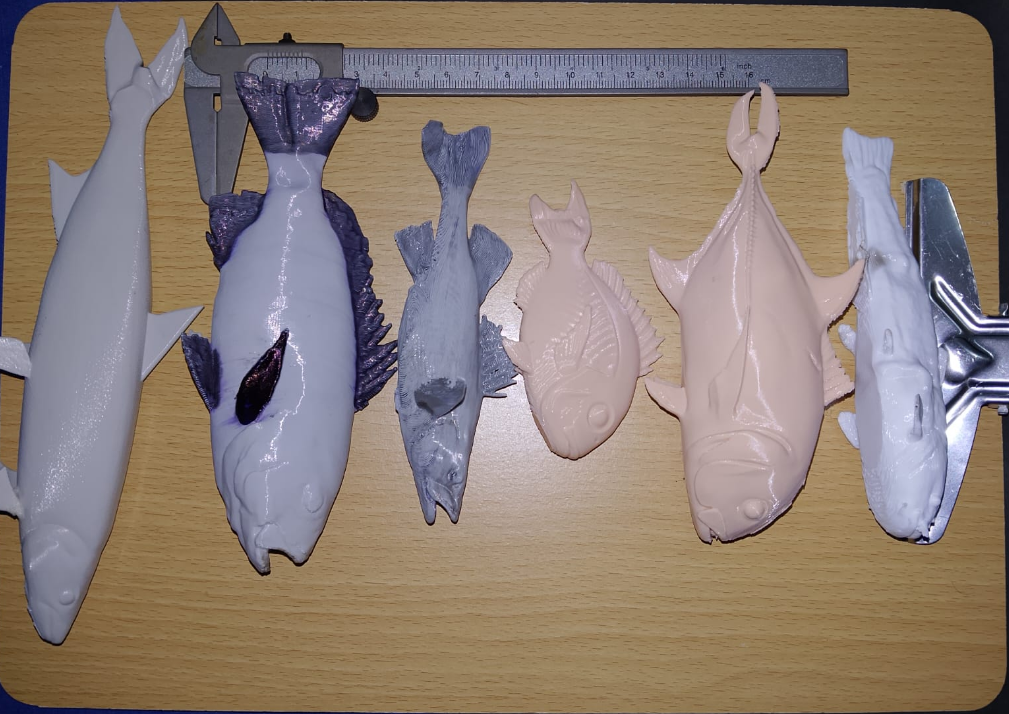
\includegraphics{figuras/originales/fig3_1_replicas.png}
\caption[Réplicas de peces impresas en PLA utilizadas en el experimento]{Réplicas de peces impresas en PLA utilizadas en el experimento. Fuente: elaboración propia.}
\label{fig:3-1}
\end{figure}

\begin{table}[htbp]

\caption{Réplicas y referencias físicas medidas con calibre.}
\label{tab:replicas}
\begin{tabular}{@{}lp{1.6cm}p{1.5cm}p{1.6cm}p{1.5cm}p{3.2cm}@{}}
\hline
Réplica & LT media (mm) & Desv. LT (mm) & PC media (mm) & Desv. PC (mm) & Origen / escala de impresión \\
\hline
R1 & \pend{ } & \pend{ } & \pend{ } & \pend{ } & \pend{ } \\
R2 & \pend{ } & \pend{ } & \pend{ } & \pend{ } & \pend{ } \\
R3 & \pend{ } & \pend{ } & \pend{ } & \pend{ } & \pend{ } \\
R4 & \pend{ } & \pend{ } & \pend{ } & \pend{ } & \pend{ } \\
R5 & \pend{ } & \pend{ } & \pend{ } & \pend{ } & \pend{ } \\
R6 & \pend{ } & \pend{ } & \pend{ } & \pend{ } & \pend{ } \\
\hline
\end{tabular}
\end{table}

\pendiente{Completar la Tabla~\ref{tab:replicas} con los valores de \texttt{lt\_reference\_mm} y \texttt{pc\_reference\_mm} del CSV maestro, la desviación entre las tres lecturas de calibre de cada réplica y el origen del modelo STL. Volver a medir la PC de R1 y R2 (tres lecturas) para resolver la inconsistencia de unidad del registro original; si los valores cambian, indicarlo con una línea en la Sección~\ref{sec:conjunto}. Cerrar el párrafo con: «La mayor desviación entre lecturas fue de X~mm, inferior al menor MAE observado».}

Cada medida de referencia se tomó tres veces con un calibre digital de resolución 0,01~mm; la media se usó como referencia y la desviación entre lecturas como repetibilidad de la referencia.

Cada réplica se ubicó con su plano de simetría a cuatro distancias nominales de la cara interna del vidrio: 5, 11, 17 y 23~cm. Estas posiciones se eligieron por los límites físicos de la pecera y por la zona en la que la imagen mantuvo un enfoque aceptable. En cada combinación de réplica y distancia se tomaron tres fotografías técnicas. Entre repeticiones no se movieron la cámara ni la pecera; se volvió a colocar la réplica en la posición indicada y se realizó una nueva captura. El orden de captura fue por réplica: se completaron sus cuatro distancias y repeticiones antes de continuar con la siguiente.

No se varió de forma planificada la posición de la réplica dentro del encuadre. Por tanto, el diseño contempló únicamente la variación de profundidad. El experimento produjo $6 \times 4 \times 3 = 72$ imágenes originales. Las repeticiones de una misma réplica se consideran repeticiones técnicas y no réplicas independientes; en consecuencia, el número de unidades experimentales es $n = 6$ y el número de combinaciones réplica--profundidad es 24.

Se incluyeron las capturas en las que la réplica se observó completamente y la imagen presentó un enfoque aceptable. Las capturas que no cumplieron estas condiciones se descartaron y el motivo se registró en la tabla maestra. La selección de la muestra responde a la disponibilidad de réplicas y al tiempo destinado al experimento, por lo que los resultados se interpretan como una evaluación experimental del montaje y no como una generalización a toda la población de peces.

\section{Montaje e instrumentos de recolección de datos}
\label{sec:montaje}

El ensayo se realizó en una pecera de aproximadamente $30 \times 30 \times 30$~cm, construida con vidrio \emph{float} de 4~mm de espesor. \pend{Indicar si el espesor se verificó con calibre (4,0~mm); en la versión anterior se verificó con una regla.} Se utilizó agua clara de la canilla. Para el modelo óptico se adoptaron los valores $\mu_a = 1{,}000$, $\mu_g = 1{,}500$ y $\mu_w = 1{,}333$; estos son valores tabulados y no mediciones directas del índice del agua. La Figura~\ref{fig:3-esquema} presenta el esquema acotado del montaje.

\begin{figure}[htbp]
\centering
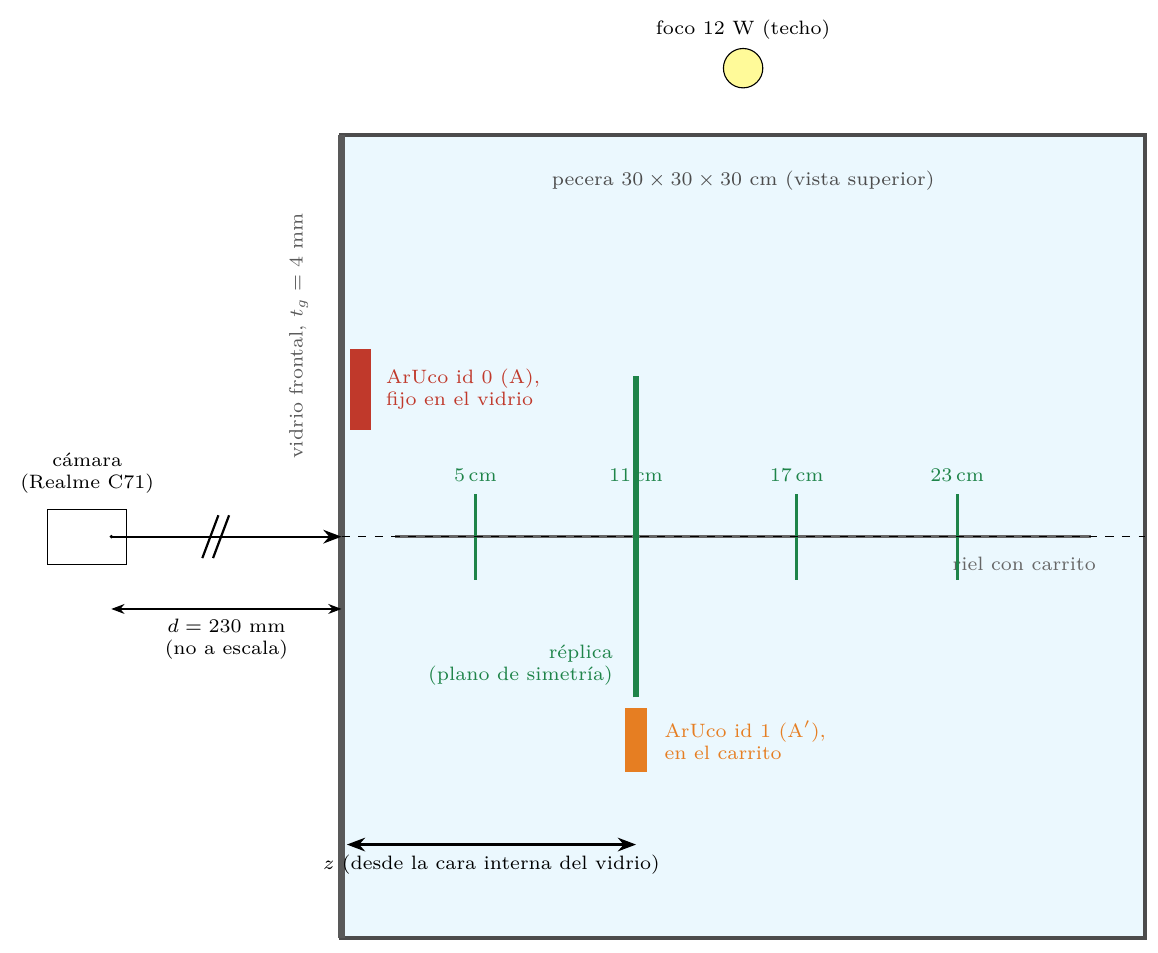
\includegraphics[width=\textwidth]{figuras/tikz/tikz_3.png}
\caption[Esquema acotado del montaje experimental]{Esquema acotado del montaje experimental en vista superior: cámara a $d = 230$~mm del vidrio frontal de 4~mm, marcador ArUco fijo en el vidrio (ruta A), riel con carrito y cuatro posiciones nominales (5, 11, 17 y 23~cm), marcador coplanar en el carrito (ruta \Aprime) e iluminación cenital fija. No está a escala. Fuente: elaboración propia.}
\label{fig:3-esquema}
\end{figure}

La cámara fue la integrada en un teléfono Realme C71 RMX5303 Dual. Las capturas se guardaron en formato JPG a $4096 \times 3072$ píxeles, con la configuración bloqueada durante el ensayo: ISO 640, velocidad de obturación 1/25~s, enfoque 0,76 y balance de blancos 5600~K. La distancia entre el frente de la lente y el vidrio fue de 230~mm, medida con una regla. Esta distancia se utilizó como aproximación de la distancia entre el centro de proyección y la primera interfaz óptica; el desplazamiento entre el frente de la lente y el centro de proyección es de pocos milímetros en una cámara de teléfono, y su efecto sobre C se cuantifica en la Sección~\ref{sec:sensibilidad} mediante el análisis de sensibilidad a $d$. La perpendicularidad aproximada del eje de la cámara respecto del vidrio se comprobó con una escuadra.

La iluminación se mantuvo fija mediante un foco de bajo consumo de 12~W ubicado en el techo de la habitación, con la pecera colocada debajo. La réplica se sostuvo mediante un riel con carrito fabricado en PLA. El soporte permitió repetir las posiciones de profundidad y mantener la réplica en una orientación similar entre capturas. La Tabla~\ref{tab:posiciones} relaciona la posición nominal de cada captura con la lectura del riel y con el origen del sistema de coordenadas usado por B.

\begin{table}[htbp]

\caption{Correspondencia entre la posición nominal de la réplica y la lectura del riel.}
\label{tab:posiciones}
\begin{tabular}{@{}p{2.8cm}p{3.4cm}p{2.6cm}p{3.4cm}@{}}
\hline
Posición nominal (cm al vidrio) & Separación de la zona de calibración de B (cm) & Lectura del riel (mm) & Desplazamiento al plano de simetría (mm) \\
\hline
5  & 0  & 0   & \pend{ } \\
11 & 6  & 60  & \pend{ } \\
17 & 12 & 120 & \pend{ } \\
23 & 18 & 180 & \pend{ } \\
\hline
\end{tabular}
\end{table}

\pendiente{Confirmar en los YAML y en el archivo maestro la lectura del riel asociada a cada posición nominal (el plano de referencia de B tiene $z_{\mathrm{ref}} = 0$ en la posición de 5~cm) y el desplazamiento entre el apoyo del carrito y el plano de simetría de cada réplica. Esta tabla responde de antemano la pregunta «¿cómo sabe la distancia al vidrio?».}

Se emplearon marcadores ArUco del diccionario \texttt{4X4\_50}, con los identificadores 0 y 1. El marcador utilizado por A permaneció fijo en el vidrio. El marcador utilizado por \Aprime{} se colocó en una base común con la réplica. Para aproximar la coplanaridad con el plano de simetría se utilizó un separador de isopor de longitud equivalente al eje de simetría, fijado con cinta impermeable de doble faz. La réplica se sujetó a la base mediante el alambre previsto en sus orificios. \pend{Indicar el lado físico medido con calibre de cada marcador (id 0 e id 1).} La Figura~\ref{fig:3-2} muestra la disposición de una réplica y del marcador coplanar dentro de la pecera.

\begin{figure}[htbp]
\centering
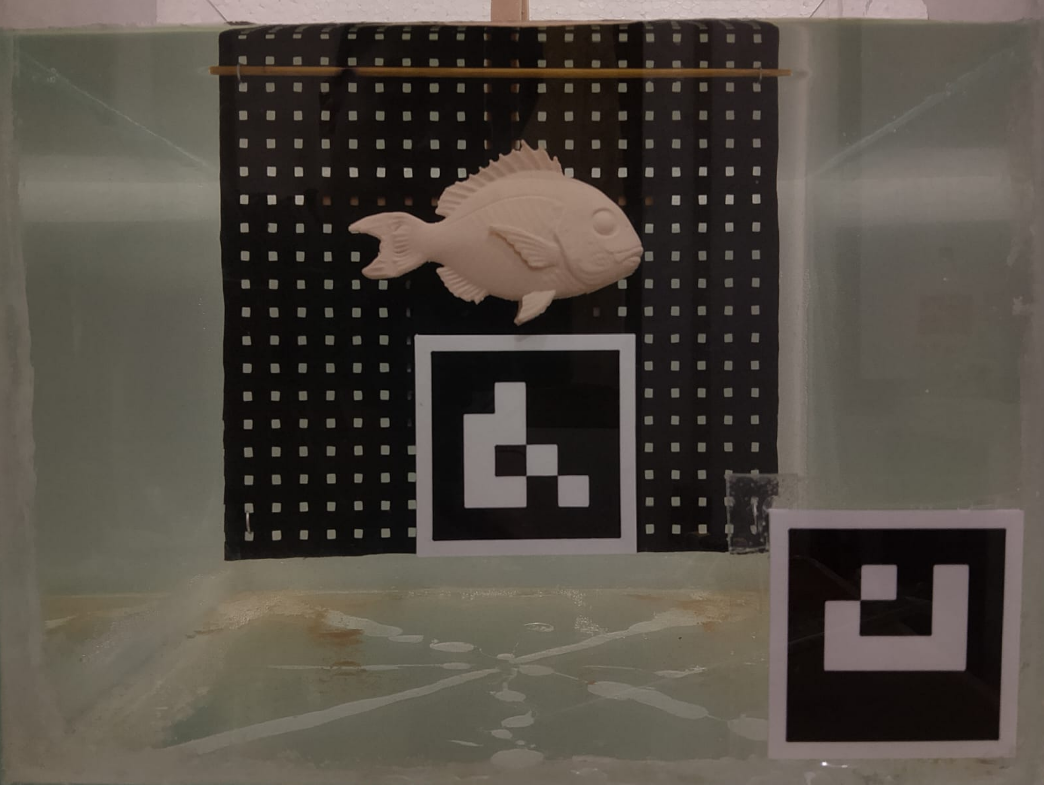
\includegraphics{figuras/originales/fig3_2_montaje_replica.png}
\caption[Montaje de una réplica junto con el marcador ArUco coplanar]{Montaje de una réplica junto con el marcador ArUco coplanar. Fuente: elaboración propia.}
\label{fig:3-2}
\end{figure}

Para la calibración se utilizó un damero de ajedrez de $5 \times 5$ cuadros ($4 \times 4$ esquinas interiores), con cuadros de 20~mm. La calibración de B se realizó en la posición más cercana al vidrio, correspondiente a la distancia nominal de 5~cm. La separación de una captura respecto de esa zona se expresó como la diferencia absoluta entre su distancia al vidrio y la distancia de calibración. La Figura~\ref{fig:3-3} presenta el damero y el marcador empleados en la preparación de la calibración.

\begin{figure}[htbp]
\centering
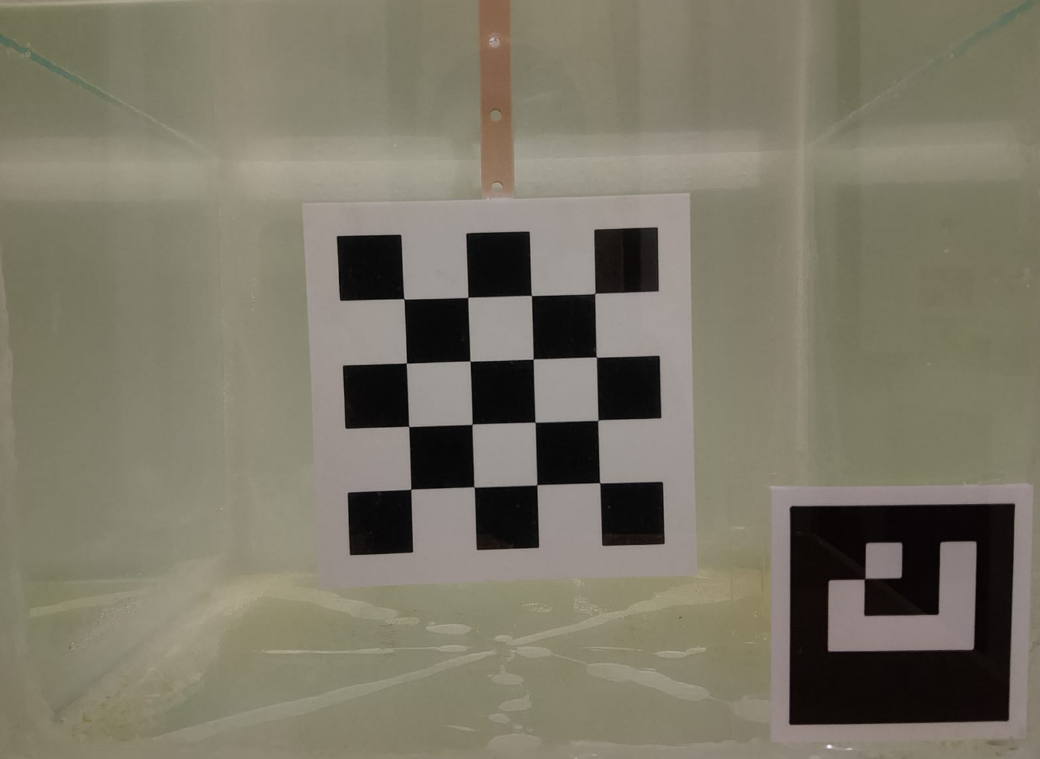
\includegraphics{figuras/originales/fig3_3_damero.png}
\caption[Damero y marcador ArUco colocados dentro de la pecera]{Damero y marcador ArUco colocados dentro de la pecera. Fuente: elaboración propia.}
\label{fig:3-3}
\end{figure}

Los parámetros físicos del puerto plano consumidos por C se resumen en la Tabla~\ref{tab:puerto}; son la ficha del instrumento y se conservan en el archivo de configuración reproducido en el Anexo~\ref{anx:flatport}.

\begin{table}[htbp]

\caption{Parámetros del puerto plano utilizados por la ruta C.}
\label{tab:puerto}
\begin{tabular}{@{}p{3.6cm}p{2.6cm}p{1.2cm}p{5.4cm}@{}}
\hline
Parámetro & Valor & Unidad & Cómo se obtuvo \\
\hline
Normal del puerto $\mathbf{n}_\pi$ & $(0, 0, 1)$ & --- & Supuesta perpendicular; comprobada con escuadra \\
Distancia cámara--vidrio $d$ & 230 & mm & Regla, desde el frente de la lente \\
Espesor del vidrio $t_g$ & 4 & mm & Regla \pend{(calibre)} \\
Índice del aire $\mu_a$ & 1,000 & --- & Valor tabulado \\
Índice del vidrio $\mu_g$ & 1,500 & --- & Valor tabulado (vidrio \emph{float}) \\
Índice del agua $\mu_w$ & 1,333 & --- & Valor tabulado (agua dulce, 22~\si{\celsius}) \\
Condiciones del agua & 22~\si{\celsius}; salinidad 0; 0~dbar & --- & Registradas en la configuración \\
\hline
\end{tabular}
\end{table}

La referencia geométrica del plano de medición de B se obtuvo a partir de dos posiciones del riel (0 y 180~mm) observadas con el damero; sus valores principales se resumen en la Tabla~\ref{tab:riel} y el archivo completo se reproduce en el Anexo~\ref{anx:riel}. El residuo del ajuste de la dirección del riel ($1{,}62 \times 10^{-13}$~mm) corresponde a una recta por dos puntos y es un residuo numérico, no una medida de precisión física; los valores de 1,0~px y $1{,}0^{\circ}$ son los umbrales de aceptación configurados para la reproyección y para la dispersión de la normal. \pend{Verificar en el código si 1,0~px y $1{,}0^{\circ}$ son tolerancias configuradas o errores observados, y ajustar la frase.}

\begin{table}[htbp]

\caption{Referencia geométrica del riel utilizada por la ruta B.}
\label{tab:riel}
\begin{tabular}{@{}p{6cm}p{7cm}@{}}
\hline
Campo & Valor \\
\hline
Plano de referencia $z_{\mathrm{ref}}$ & 0,0~mm (posición nominal de 5~cm) \\
Posiciones del riel utilizadas & 0,0 y 180,0~mm \\
Umbral de reproyección & 1,0~px \\
Umbral de dispersión de la normal & $1{,}0^{\circ}$ \\
Error relativo de escala informado & 0,813~\% \\
Supuesto & Planos de las réplicas paralelos al tablero \\
\hline
\end{tabular}
\end{table}

\section{Software utilizado}
\label{sec:software}

El procesamiento se realizó con la aplicación de escritorio Fishmeter, desarrollada en Python 3.12. Su código fuente y la documentación de uso se encuentran disponibles en el repositorio público \url{\RepoURL}. La aplicación utiliza OpenCV 5.0.0 para la detección de marcadores, la calibración y las transformaciones geométricas; NumPy para las operaciones vectoriales; PyYAML para los archivos de configuración; y Tkinter (biblioteca estándar) para la interfaz gráfica. \pend{Agregar las versiones de NumPy y PyYAML del \texttt{requirements.txt} congelado.} La versión utilizada corresponde a la etiqueta \texttt{\RepoTag} del repositorio (commit \texttt{\RepoCommitShort}). \pend{Crear la etiqueta \texttt{v1.0-tesis} sobre el commit final con los datos publicados y actualizar el hash si cambia.}

El módulo refractivo (\texttt{refractive\_port.py} y \texttt{snells\_law.py}) implementa las ecuaciones~\eqref{eq:va} a~\eqref{eq:rayo} y cuenta con pruebas unitarias de sanidad: con $\mu_g = \mu_w = 1$ y $t_g = 0$ reproduce la cámara pinhole, y un rayo sobre el eje óptico no se desvía. Las pruebas de integración verifican que los cuatro métodos reciben las mismas coordenadas y producen un registro trazable por imagen.

La interfaz permite cargar la fotografía, detectar los marcadores, cargar o seleccionar manualmente los puntos anatómicos, ejecutar los cuatro métodos y exportar sus resultados. Los clics realizados sobre el visor se convierten a coordenadas de la imagen original antes de ser guardados o procesados. La Figura~\ref{fig:3-4} muestra la pantalla utilizada para la selección de puntos y la comparación de las mediciones.

\begin{figure}[htbp]
\centering
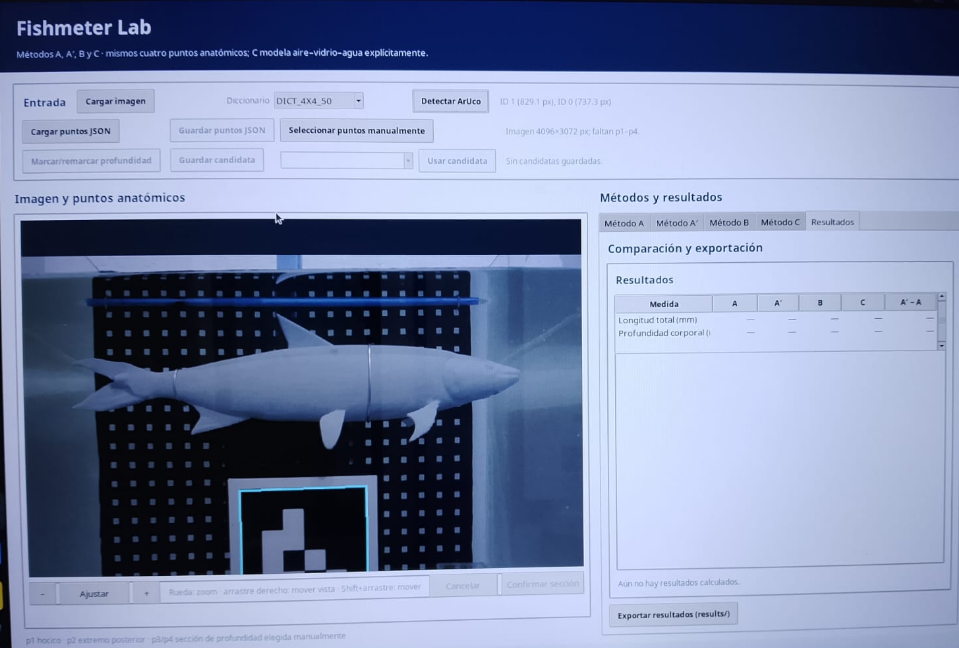
\includegraphics{figuras/originales/fig3_4_interfaz.png}
\caption[Interfaz de Fishmeter para la marcación y comparación de métodos]{Interfaz de Fishmeter para la marcación y comparación de métodos. Fuente: Fishmeter.}
\label{fig:3-4}
\end{figure}

\section{Medidas físicas, puntos anatómicos y variables}
\label{sec:medidas}

Para cada réplica se conservaron medidas físicas de referencia de la longitud total y de la profundidad corporal (Tabla~\ref{tab:replicas}). La referencia y la imagen utilizaron la misma convención anatómica, definida en la Sección~\ref{sec:puntos-def}. La longitud total se definió entre el extremo anterior del hocico ($\mathbf{p}_1$) y el punto más posterior de la aleta caudal sobre el eje longitudinal ($\mathbf{p}_2$); cuando la cola presenta dos lóbulos, $\mathbf{p}_2$ es el extremo del lóbulo de mayor longitud. La profundidad corporal se midió entre el perfil dorsal ($\mathbf{p}_3$) y el perfil ventral ($\mathbf{p}_4$) de una misma sección transversal, sin incluir las aletas.

Los cuatro puntos se marcaron manualmente sobre la imagen original. El eje longitudinal de la réplica se indicó de forma explícita y se utilizó para proyectar las medidas. No se empleó segmentación automática ni se eligieron puntos diferentes para cada método. La Figura~\ref{fig:3-5} resume la ubicación de los cuatro puntos y las dos medidas consideradas, y la Figura~\ref{fig:3-6} presenta los instrumentos utilizados para obtener las dimensiones físicas de referencia.

\begin{figure}[htbp]
\centering
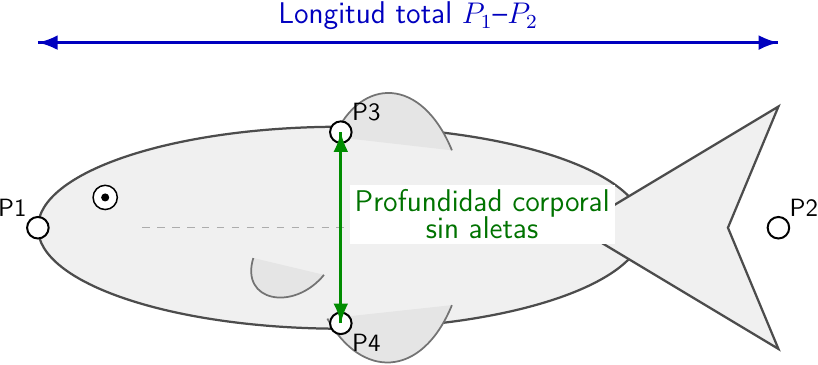
\includegraphics{figuras/originales/fig3_5_puntos.png}
\caption[Puntos anatómicos empleados para la longitud total y la profundidad corporal]{Puntos anatómicos empleados para la longitud total y la profundidad corporal. Fuente: elaboración propia.}
\label{fig:3-5}
\end{figure}

\begin{figure}[htbp]
\centering
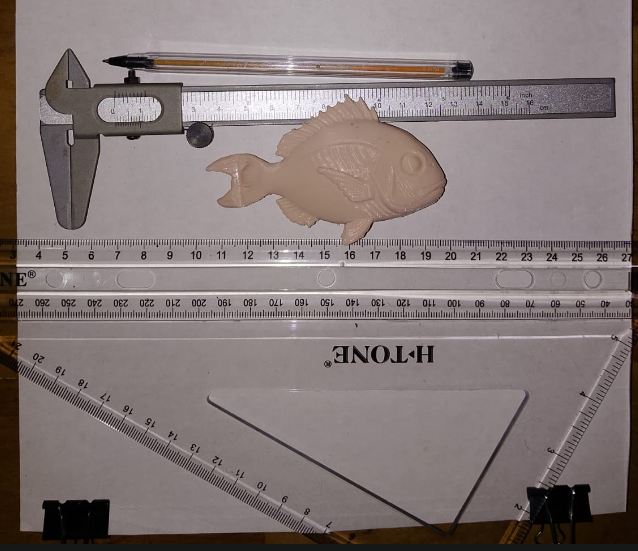
\includegraphics{figuras/originales/fig3_6_instrumentos.png}
\caption[Instrumentos y disposición utilizados para medir físicamente una réplica]{Instrumentos y disposición utilizados para medir físicamente una réplica. Fuente: elaboración propia.}
\label{fig:3-6}
\end{figure}

Si $\mathbf{u}$ es el vector unitario del eje longitudinal y $\mathbf{n} = (-u_y, u_x)$ su normal, las medidas en el plano métrico se calcularon como
\begin{equation}
\mathrm{LT} = \lvert (\mathbf{q}_2 - \mathbf{q}_1)\cdot\mathbf{u} \rvert, \qquad
\mathrm{PC} = \lvert (\mathbf{q}_4 - \mathbf{q}_3)\cdot\mathbf{n} \rvert,
\label{eq:medidas}
\end{equation}
donde $\mathbf{q}_i$ son los puntos anatómicos ya convertidos a milímetros por la ruta correspondiente. Operacionalmente, LT es la proyección del segmento $\mathbf{p}_1$--$\mathbf{p}_2$ sobre el eje longitudinal; con los puntos sobre el eje coincide con la distancia euclídea, que es la convención usada con el calibre. La profundidad solo se aceptó cuando la sección marcada fue suficientemente perpendicular al eje. La aplicación conservó como diagnóstico el desvío de la sección y permitió descartar una profundidad no válida.

La Tabla~\ref{tab:operacionalizacion} presenta la definición conceptual y operacional de las variables del estudio, separando los factores que se variaron, los resultados que se midieron y las condiciones que se mantuvieron fijas.

\begin{table}[htbp]

\caption{Operacionalización de las variables.}
\label{tab:operacionalizacion}
\begin{tabular}{@{}p{2.3cm} p{1.3cm} X X p{1.2cm}@{}}
\hline
Variable & Tipo & Definición conceptual & Definición operacional & Unidad \\
\hline
\multicolumn{5}{@{}l}{\emph{Factores variados}}\\
Método & Nominal & Ruta de conversión píxel--milímetro & A, \Aprime, B o C aplicados a los mismos puntos (Sección~\ref{sec:metodos}) & --- \\
Distancia al vidrio & Nominal & Profundidad $z$ del plano de simetría de la réplica & Posición del carrito: 5, 11, 17 o 23~cm; separación de la zona de B: 0, 6, 12 o 18~cm & cm \\
Rango de $z$ & Nominal & Conocimiento disponible sobre la profundidad & Toda la pecera (0--30~cm); $\pm 3$~cm; $\pm 1$~cm & cm \\
\multicolumn{5}{@{}l}{\emph{Resultados medidos}}\\
LT y PC estimadas & Razón & Longitud total y profundidad corporal de la réplica & Salida de Fishmeter por método, ecuación~\eqref{eq:medidas} & mm \\
LT y PC de referencia & Razón & Dimensión física de la réplica & Media de tres lecturas con calibre digital (0,01~mm) & mm \\
Error con signo, EA, EPA & Razón & Diferencia entre estimación y referencia & Ecuaciones~\eqref{eq:errores} & mm, mm, \% \\
Ancho relativo de $\IL$ & Razón & Extensión del intervalo por profundidad desconocida & $(\max_z L - \min_z L)/\mathrm{LT}_{\mathrm{ref}}$ & \% \\
Cobertura de $\IL$ & Razón & Fracción de capturas cuya referencia cae en $\IL$ & Conteo sobre las capturas disponibles & --- \\
\multicolumn{5}{@{}l}{\emph{Condiciones fijas}}\\
Cámara, pecera, agua, luz, marcadores, soporte, operador & --- & Condiciones del montaje & Registradas en las Secciones~\ref{sec:montaje} y~\ref{sec:procedimiento} & --- \\
\hline
\end{tabular}
\end{table}

\section{Métodos de conversión métrica}
\label{sec:metodos}

Cada método recibe la misma imagen, los mismos cuatro puntos y el mismo eje. Solo cambia la transformación utilizada para convertir píxeles a milímetros.

\begin{description}
  \item[Método A.] Utiliza el ArUco fijo en el vidrio. Con el lado físico $L_m$ del marcador y el promedio $\bar{p}$ de las longitudes en píxeles de sus cuatro lados (ecuación~\ref{eq:lado}), la escala implementada es
  \begin{equation}
    k = \frac{L_m}{\bar{p}}, \qquad \bar{p} = \frac{1}{4}\sum_{i=1}^{4} p_i,
    \label{eq:escala-impl}
  \end{equation}
  que difiere de la ecuación~\eqref{eq:escala-monkman} en el orden del promedio; para marcadores bien detectados ambas coinciden hasta la tercera cifra. Cada punto se transforma como $\mathbf{q}_i = k\,\mathbf{p}_i$ y las medidas se obtienen con la ecuación~\eqref{eq:medidas}. Es una línea de base que no corrige la diferencia de profundidad entre el vidrio y la réplica.
  \item[Método \Aprime.] Utiliza el ArUco montado aproximadamente en el plano de simetría de la réplica. Las cuatro esquinas del marcador en píxeles y sus coordenadas métricas $(0,0)$, $(L_m,0)$, $(L_m,L_m)$ y $(0,L_m)$ definen una homografía $\mathbf{H}$ de $3 \times 3$; cada punto anatómico se transforma como $\tilde{\mathbf{q}}_i = \mathbf{H}\,\tilde{\mathbf{p}}_i$ en milímetros sobre el plano del marcador, el eje longitudinal se transforma del mismo modo, y las medidas se calculan con la ecuación~\eqref{eq:medidas}. La homografía corrige la perspectiva dentro del plano del marcador, pero no la diferencia de escala de puntos fuera de ese plano.
  \item[Método B.] Utiliza la calibración de cámara con el damero sumergido y un modelo pinhole efectivo (perfil \texttt{B-effective}, Anexo~\ref{anx:calibraciones}). Los píxeles se convierten en rayos con $\mathbf{K}_{\mathrm{agua}}$ y los coeficientes de distorsión efectivos (ecuaciones~\ref{eq:pinhole} y~\ref{eq:distorsion}, invertidas) y se intersecan con el plano $\pi_z$, paralelo al tablero de calibración, situado a la distancia nominal del carrito más el desplazamiento al plano de simetría (Tabla~\ref{tab:posiciones}). La calibración se fijó en la posición más cercana al vidrio, de modo que B representa de forma empírica el comportamiento óptico de la zona calibrada. LT y PC se calculan en el espacio métrico tridimensional.
  \item[Método C.] Utiliza la calibración de cámara en aire (perfil \texttt{C-air}) y el modelo de puerto plano de la Sección~\ref{sec:puerto-plano}. Para cada punto se corrige la distorsión de lente, se obtiene el rayo en aire (ecuación~\ref{eq:va}), se aplican las dos refracciones (ecuaciones~\ref{eq:q1} a~\ref{eq:vw}) con los parámetros de la Tabla~\ref{tab:puerto} y se interseca el rayo en agua (ecuación~\ref{eq:rayo}) con el plano de la réplica, definido en el marco de la cámara física. Para estudiar el caso de profundidad desconocida, el mismo cálculo se repite sobre la grilla de profundidades físicamente admisibles y se expresa como el intervalo geométrico de la ecuación~\eqref{eq:IL}.
\end{description}

La prueba complementaria con una barra patrón sumergida, prevista para separar un eventual error de implementación del error de marcado, no se realizó como validación separada; se efectuó únicamente una comprobación preliminar sobre la réplica R1 (longitud aproximada de 160~mm). La validación métrica de las cuatro rutas en este trabajo es la comparación directa con las longitudes y profundidades de calibre de las seis réplicas en las cuatro posiciones (Capítulo~\ref{cap:resultados}). En este documento se distingue «comprobación instrumental con patrón» (barra sumergida, no realizada) de «validación externa» (otras cámaras, montajes o condiciones, fuera del alcance).

\section{Procedimiento por imagen y trazabilidad}
\label{sec:procedimiento}

El procesamiento siguió la secuencia de la Figura~\ref{fig:3-flujo}, idéntica para las 72 imágenes:

\begin{enumerate}
  \item identificar la réplica, la distancia y la repetición, y conservar la imagen JPG original;
  \item verificar visibilidad y enfoque;
  \item marcar manualmente $\mathbf{p}_1$, $\mathbf{p}_2$, $\mathbf{p}_3$ y $\mathbf{p}_4$ en coordenadas de la imagen original;
  \item registrar el eje longitudinal y las observaciones de calidad;
  \item aplicar A, \Aprime, B y C a las mismas coordenadas;
  \item calcular LT y PC en milímetros y guardar advertencias o exclusiones;
  \item asociar cada estimación con la referencia física, la calibración, la versión del procedimiento y el nombre de la imagen.
\end{enumerate}

\begin{figure}[htbp]
\centering
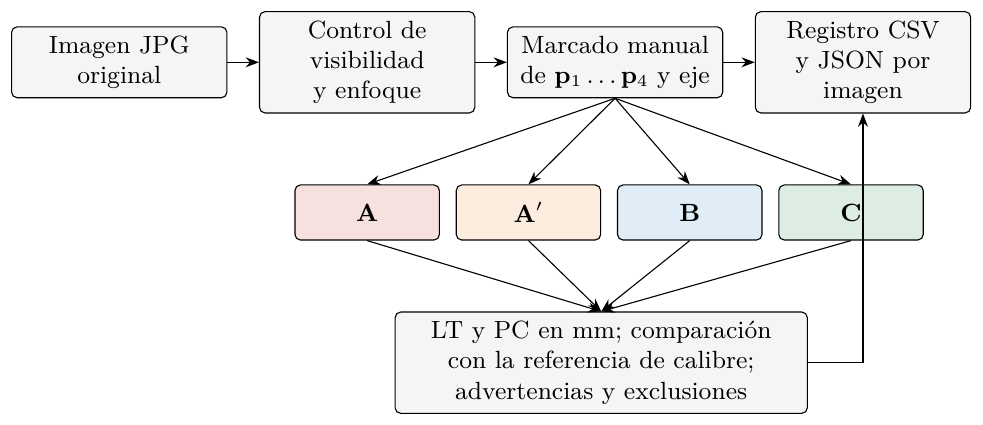
\includegraphics[width=\textwidth]{figuras/tikz/tikz_4.png}
\caption[Flujo de procesamiento por imagen]{Flujo de procesamiento por imagen: los mismos cuatro puntos marcados una sola vez alimentan las cuatro rutas, y cada estimación queda asociada a su referencia física y a su registro. Fuente: elaboración propia.}
\label{fig:3-flujo}
\end{figure}

La tabla maestra incluyó el identificador de la réplica y de la imagen, distancia al vidrio, repetición, método, medida, referencia física, estimación, error, estado de los puntos, estado del marcador y motivo de exclusión cuando correspondió. De este modo, cada estimación pudo rastrearse hasta la fotografía original y sus coordenadas manuales. Los archivos de datos (imágenes, puntos, calibraciones y tabla maestra) y el script que regenera las tablas y figuras del Capítulo~\ref{cap:resultados} forman parte del repositorio (Anexo~\ref{anx:repositorio}).

\section{Evaluación de las estimaciones}
\label{sec:evaluacion}

Para cada medida se calculó el error con signo, el error absoluto y el error porcentual absoluto:
\begin{equation}
e = \hat{y} - y, \qquad \mathrm{EA} = \lvert \hat{y} - y \rvert, \qquad \mathrm{EPA} = 100\,\frac{\lvert \hat{y} - y \rvert}{y},
\label{eq:errores}
\end{equation}
donde $\hat{y}$ es la estimación del método y $y$ la referencia física. Las tres repeticiones técnicas se resumieron por réplica y distancia antes de comparar los métodos, evitando tratarlas como observaciones independientes. Sobre las $n = 24$ combinaciones réplica--profundidad se calcularon el sesgo, el error absoluto medio y el error porcentual absoluto medio:
\begin{equation}
\mathrm{sesgo} = \frac{1}{n}\sum_{i=1}^{n} e_i, \qquad
\mathrm{MAE} = \frac{1}{n}\sum_{i=1}^{n} \lvert e_i \rvert, \qquad
\mathrm{MAPE} = \frac{100}{n}\sum_{i=1}^{n} \frac{\lvert e_i \rvert}{y_i}.
\label{eq:agregados}
\end{equation}
Un sesgo positivo indica sobreestimación y uno negativo subestimación. Estas métricas describen la estimación promedio por condición; el error de una captura individual puede ser mayor. \pend{Si se dispone del CSV, reportar también el MAE calculado sobre las capturas individuales como columna adicional de la Tabla~\ref{tab:agregados}.}

La comparación principal se organizó mediante el error de A, \Aprime, B y C para las mismas imágenes y profundidades. Como las 24 combinaciones pertenecen a seis réplicas (medidas repetidas), la inferencia se hizo con la réplica como unidad: para cada réplica se promedió el error absoluto de LT sobre las cuatro posiciones y se aplicó una prueba de signos exacta, de dos colas, a las diferencias pareadas entre C y cada uno de los otros métodos ($n = 6$). No se aplicaron pruebas paramétricas porque seis réplicas no permiten verificar sus supuestos. Los conteos por combinación réplica--profundidad (24 pares) se reportan como descriptivos. También se consideró el cambio del error de B y C al aumentar la separación respecto de la calibración de B, resumido por la pendiente de una recta ajustada por mínimos cuadrados a la diferencia de MAE frente a la separación.

Para C se consideró el intervalo de longitudes obtenido al recorrer las profundidades admisibles. Ese intervalo representa incertidumbre geométrica por profundidad y no un intervalo de confianza estadístico. Su ancho relativo se evaluó para tres escenarios de conocimiento de $z$ (toda la pecera, $\pm 3$~cm y $\pm 1$~cm) y se comparó con la predicción de primer orden de la ecuación~\eqref{eq:Dz}. La concordancia entre C y la referencia se describe además con el sesgo y los límites de acuerdo de Bland--Altman \parencite{Bland1986}. \pend{Calcular los límites de acuerdo a partir del CSV maestro e incluir la figura correspondiente en la Sección~\ref{sec:discusion}.}

\section{Alcance y limitaciones metodológicas}
\label{sec:limitaciones-metod}

El procedimiento mide réplicas rígidas y utiliza localización manual de puntos; por ello no representa un sistema de segmentación automática ni una medición completamente automática. La distancia cámara--vidrio se midió desde el frente de la lente y los índices de refracción se tomaron de valores tabulados; la sensibilidad de C a estos dos parámetros se cuantifica en la Sección~\ref{sec:sensibilidad}. La referencia del plano de B depende del ajuste del riel (Tabla~\ref{tab:riel}), cuyo error relativo de escala informado (0,813~\%) se retoma al interpretar el sesgo de B. La comprobación instrumental con una barra patrón sumergida no se realizó; la validación métrica del trabajo es la comparación con las referencias de calibre de las réplicas.

\section{Cuestiones éticas y uso de herramientas}
\label{sec:etica}

No se utilizaron animales ni datos de terceros; las réplicas, las imágenes, las calibraciones y las medidas son propias. El código de la aplicación, incluido el módulo refractivo, fue desarrollado por el autor y su historial de versiones está disponible en el repositorio. Durante la redacción se emplearon herramientas de asistencia basadas en modelos de lenguaje para revisar la estructura del documento, la consistencia de la notación y la redacción de borradores de secciones a partir de los datos del autor; el diseño experimental, la captura, el marcado, el análisis y las conclusiones son responsabilidad del autor, quien revisó y validó todo el texto.

\chapter{Resultados y discusión}
\label{cap:resultados}

Este capítulo presenta los resultados registrados en el CSV maestro del experimento. El análisis se realizó sobre el experimento principal, conservando la correspondencia entre cada imagen, la réplica, la profundidad, la repetición técnica y el método de conversión métrica. Las cifras se informan como una comparación dentro del montaje utilizado y contra las referencias físicas de las réplicas; no se interpretan como una validación del sistema en otras condiciones.

\section{Composición del conjunto y control de calidad}
\label{sec:conjunto}

El archivo contiene 288 registros: 72 imágenes, seis réplicas de PLA, cuatro posiciones nominales respecto del vidrio (5, 11, 17 y 23~cm), tres capturas técnicas por condición y cuatro métodos (A, \Aprime, B y C). Por cada combinación de réplica y profundidad se dispone, en general, de tres capturas. Las capturas repetidas se trataron como repeticiones técnicas y no como réplicas independientes.

Se obtuvieron valores numéricos para 284 registros. Los cuatro registros sin medición corresponden a A y \Aprime{} en dos imágenes en las que no se detectó el marcador ArUco: \texttt{R2-REP2-170.jpg} y \texttt{R3-REP2-50.jpg}. El motivo se conservó en el CSV y esos registros se excluyeron de los cálculos de error. Los métodos B y C produjeron valores para las 72 imágenes. La aplicación conserva para ambos un estado interno \texttt{PENDING\_VALIDATION}, que solo cambia cuando se registra una barra patrón sumergida; esa comprobación instrumental complementaria no se realizó (Sección~\ref{sec:metodos}). La validación métrica de B y C en este trabajo es la comparación directa con las longitudes y profundidades de calibre de las seis réplicas en las cuatro posiciones, que se presenta en las Secciones~\ref{sec:agregados} y~\ref{sec:profundidad}. La Tabla~\ref{tab:registros} resume el tratamiento de los registros.

\begin{table}[htbp]

\caption{Registros del CSV y su tratamiento en el análisis.}
\label{tab:registros}
\begin{tabular}{@{}lccp{7.5cm}@{}}
\hline
Método & Registros & Con valor & Tratamiento \\
\hline
A & 72 & 70 & Se excluyeron dos registros por falta de detección del ArUco. \\
\Aprime & 72 & 70 & Se excluyeron dos registros por falta de detección del ArUco. \\
B & 72 & 72 & Valor numérico en las 72 imágenes; evaluado contra la referencia de calibre. \\
C & 72 & 72 & Valor numérico en las 72 imágenes; evaluado contra la referencia de calibre. \\
\hline
\end{tabular}
\end{table}

En las dos combinaciones afectadas por la ausencia de ArUco, A y \Aprime{} se promediaron con las dos capturas disponibles, mientras que B y C usaron las tres; el pareamiento no es por ello idéntico en esas dos combinaciones. \pendiente{Recalcular las Tablas~\ref{tab:agregados} y~\ref{tab:posiciones-mae} usando la intersección de las 70 imágenes comunes a los cuatro métodos y reportar en una línea si el resultado cambia (o cuánto).}

\pendiente{Las referencias de profundidad corporal de R1 y R2 figuraban en el registro original con una advertencia de revisión de unidad. Volver a medirlas con calibre (tres lecturas), actualizar \texttt{pc\_reference\_mm}, recalcular las filas de PC de la Tabla~\ref{tab:agregados} y el párrafo correspondiente de la Sección~\ref{sec:profundidad}. Si los valores nuevos coinciden con los registrados, eliminar este recuadro; si cambian, reemplazarlo por: «Las referencias de PC de R1 y R2 se volvieron a medir el [fecha] por una inconsistencia de unidad en el registro original; las cifras de este capítulo usan los valores corregidos».}

\section{Calibraciones}
\label{sec:calibraciones}

Las dos calibraciones de cámara se realizaron el 12 de octubre de 2026 con el damero de $4 \times 4$ esquinas interiores y cuadros de 20~mm, a la resolución de captura de $4096 \times 3072$ píxeles. La Tabla~\ref{tab:calibraciones} resume sus indicadores de calidad; los perfiles completos se reproducen en el Anexo~\ref{anx:calibraciones}.

\begin{table}[htbp]

\caption{Calibraciones de cámara utilizadas por las rutas B y C.}
\label{tab:calibraciones}
\begin{tabular}{@{}p{4.2cm}p{4.4cm}p{4.4cm}@{}}
\hline
Campo & Perfil B (bajo agua) & Perfil C (en aire) \\
\hline
Identificador & \texttt{B-effective} & \texttt{C-air} \\
Rutina & \texttt{calibrateCamera} (OpenCV 5.0.0) & \texttt{calibrateCamera} (OpenCV 5.0.0) \\
RMS de reproyección & 0,4354~px & 0,3745~px \\
Vistas recibidas / aceptadas & 35 / 35 & 36 / 36 \\
Vistas rechazadas & 0 & 0 \\
Focal efectiva $f_x$ & 4502,3~px & 3313,7~px \\
Punto principal $(c_x, c_y)$ & (2027,3; 1549,0)~px & (2028,2; 1530,6)~px \\
\hline
\end{tabular}
\end{table}

Ambos valores de RMS están por debajo de 0,5~px, umbral habitual para una calibración aceptable, y ninguna vista fue rechazada. La razón entre las focales efectivas, $f_{x,\mathrm{agua}}/f_{x,\mathrm{aire}} = 4502{,}3/3313{,}7 = 1{,}36$, es consistente con el índice de refracción del agua ($\mu_w = 1{,}333$): la calibración de B absorbe la refracción en una focal efectiva mayor, lo que explica por qué el modelo pinhole aproxima el sistema cerca de la distancia de calibración y se aparta de él al cambiar la profundidad.

\subsection{Sensibilidad de C a los parámetros del montaje}
\label{sec:sensibilidad}

\pendiente{Ejecutar \texttt{sensitivity\_c()} sobre una imagen de cada réplica variando $d$ en $\pm 20$~\% (184 y 276~mm) y $\mu_w$ en $\pm 0{,}01$ (1,323 y 1,343), y completar la Tabla~\ref{tab:sensibilidad} con el cambio de LT en mm y en porcentaje. Cerrar con una oración del tipo: «Un error de $\pm 20$~\% en $d$ cambia LT en menos de X~mm (Y~\%), por lo que la medición con regla desde el frente de la lente no limita la exactitud de C».}

\begin{table}[htbp]

\caption{Sensibilidad de la longitud total estimada por C a los parámetros medidos a mano.}
\label{tab:sensibilidad}
\begin{tabular}{@{}p{4cm}p{2.6cm}p{2.8cm}p{2.8cm}@{}}
\hline
Parámetro & Variación & Cambio medio de LT (mm) & Cambio medio de LT (\%) \\
\hline
Distancia cámara--vidrio $d$ & $-20$~\% (184~mm) & \pend{ } & \pend{ } \\
Distancia cámara--vidrio $d$ & $+20$~\% (276~mm) & \pend{ } & \pend{ } \\
Índice del agua $\mu_w$ & $-0{,}01$ (1,323) & \pend{ } & \pend{ } \\
Índice del agua $\mu_w$ & $+0{,}01$ (1,343) & \pend{ } & \pend{ } \\
\hline
\end{tabular}
\end{table}

En la aproximación de primer orden de la ecuación~\eqref{eq:Dz}, una variación $\Delta d$ cambia la longitud estimada en una fracción $\Delta d / D(z)$; con $D(z)$ entre 270 y 405~mm para las posiciones estudiadas, un error de 10~mm en $d$ corresponde a entre 2,5 y 3,7~\% de LT, lo que acota el efecto esperado mientras se completa la tabla.

\section{Resultados agregados por método}
\label{sec:agregados}

Las métricas se calcularon según la Sección~\ref{sec:evaluacion} después de promediar las tres capturas de cada combinación réplica--profundidad, de modo que la comparación principal quedó formada por 24 combinaciones por método. La Tabla~\ref{tab:agregados} resume las diferencias entre las estimaciones promediadas y sus referencias físicas, y la Figura~\ref{fig:4-1} las presenta gráficamente. A presenta sesgo negativo en ambas medidas, mientras que \Aprime, B y C tienden a sobreestimar. C obtiene el menor MAE y MAPE en LT y PC; \Aprime{} presenta el segundo mejor comportamiento. B queda por encima de ambos en error medio, y A es el método más afectado.

\begin{table}[htbp]

\caption{Errores medios por método después de resumir las repeticiones técnicas.}
\label{tab:agregados}
\begin{tabular}{@{}lccccccc@{}}
\hline
Método & $n$ & Sesgo LT & MAE LT & MAPE LT & Sesgo PC & MAE PC & MAPE PC \\
 & & (mm) & (mm) & (\%) & (mm) & (mm) & (\%) \\
\hline
A       & 24 & $-37{,}43$ & 37,43 & 25,68 & $-9{,}07$ & 9,07 & 25,25 \\
\Aprime & 24 & $+3{,}29$  & 3,29  & 2,28  & $+0{,}95$ & 1,03 & 2,78 \\
B       & 24 & $+16{,}32$ & 16,32 & 11,24 & $+3{,}68$ & 3,68 & 9,96 \\
C       & 24 & $+1{,}07$  & 1,22  & 0,88  & $+0{,}29$ & 0,56 & 1,62 \\
\hline
\end{tabular}



\emph{Nota.} $n$ es el número de combinaciones réplica--profundidad, no el número de fotografías. Las métricas describen la estimación promedio por condición.

\end{table}

\begin{figure}[htbp]
\centering
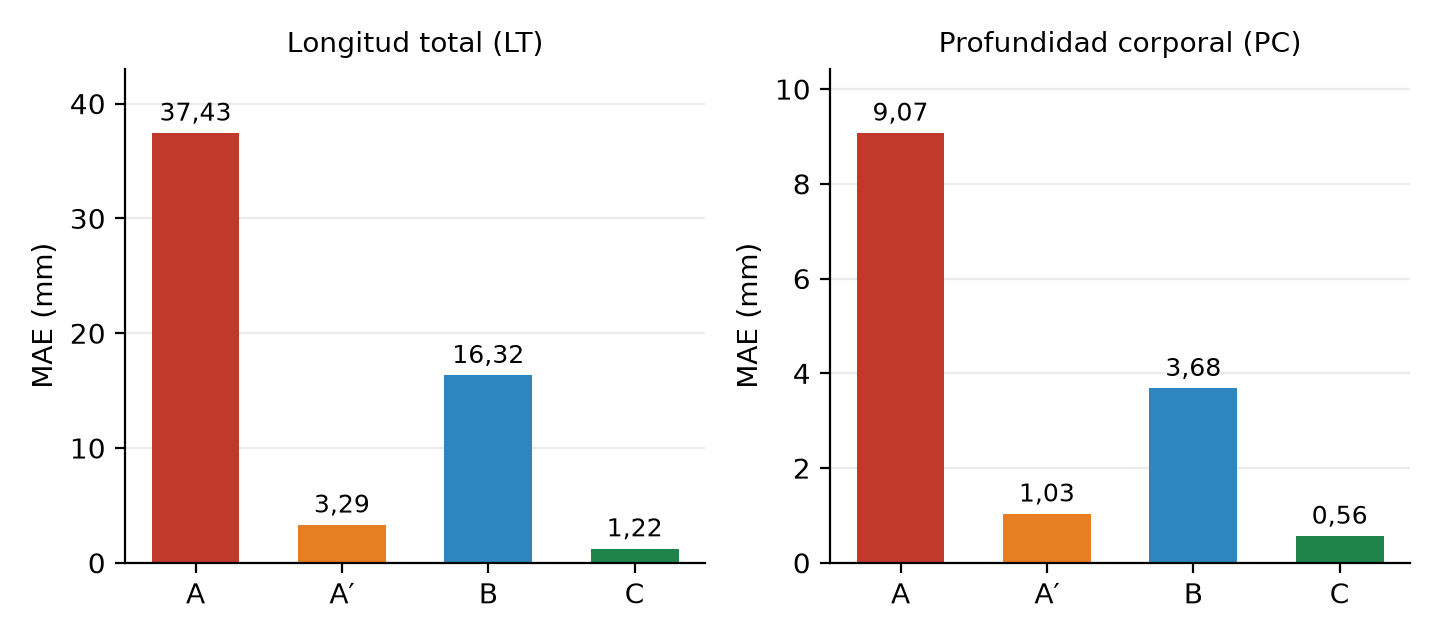
\includegraphics{figuras/fig4_1_mae_por_metodo.png}
\caption[MAE por método para longitud total y profundidad corporal]{Error absoluto medio por método para longitud total (izquierda) y profundidad corporal (derecha), sobre las 24 combinaciones réplica--profundidad (datos de la Tabla~\ref{tab:agregados}). Fuente: elaboración propia.}
\label{fig:4-1}
\end{figure}

En LT, A subestimó en promedio 37,43~mm, mientras que B sobreestimó 16,32~mm. La homografía de \Aprime{} redujo el MAE a 3,29~mm y el modelo C a 1,22~mm. En PC se observó el mismo orden general: A alcanzó un MAE de 9,07~mm, B de 3,68~mm, \Aprime{} de 1,03~mm y C de 0,56~mm. La diferencia entre C y \Aprime{} fue menor en PC que en LT, pero C tuvo menor MAE de PC en 21 de las 24 combinaciones.

La comparación pareada de LT mostró que C tuvo menor error absoluto que A, \Aprime{} y B en las 24 combinaciones disponibles. Para PC, C fue mejor que A y B en las 24 combinaciones y mejor que \Aprime{} en 21. Con la réplica como unidad experimental, C tuvo menor error absoluto medio de LT que cada uno de los otros tres métodos en las seis réplicas; la prueba de signos exacta de dos colas sobre las seis diferencias pareadas da $p = 2/2^{6} = 0{,}031$ para cada comparación. Los conteos sobre las 24 combinaciones se reportan como descriptivos porque las combinaciones de una misma réplica no son independientes. \pend{Completar para PC: C fue mejor que \Aprime{} en $k$ de 6 réplicas ($p = \ldots$).}

\section{Comportamiento según la profundidad}
\label{sec:profundidad}

La dependencia con la distancia al vidrio se aprecia con mayor claridad en la longitud total. La Tabla~\ref{tab:posiciones-mae} presenta el MAE de LT para cada posición, calculado después de promediar las repeticiones técnicas, y la Figura~\ref{fig:4-2} muestra las cuatro curvas.

\begin{table}[htbp]

\caption{MAE de longitud total (mm) por posición de la réplica.}
\label{tab:posiciones-mae}
\begin{tabular}{@{}p{1.6cm}p{2.6cm}ccccc@{}}
\hline
Distancia (cm) & Separación de la zona de B (cm) & A & \Aprime & B & C & B $-$ C \\
\hline
5  & 0  & 13,77 & 3,44 & 19,43 & 1,09 & 18,34 \\
11 & 6  & 32,02 & 3,18 & 17,45 & 1,41 & 16,04 \\
17 & 12 & 46,29 & 3,44 & 15,26 & 1,30 & 13,96 \\
23 & 18 & 57,64 & 3,11 & 13,16 & 1,07 & 12,09 \\
\hline
\end{tabular}
\end{table}

\begin{figure}[htbp]
\centering
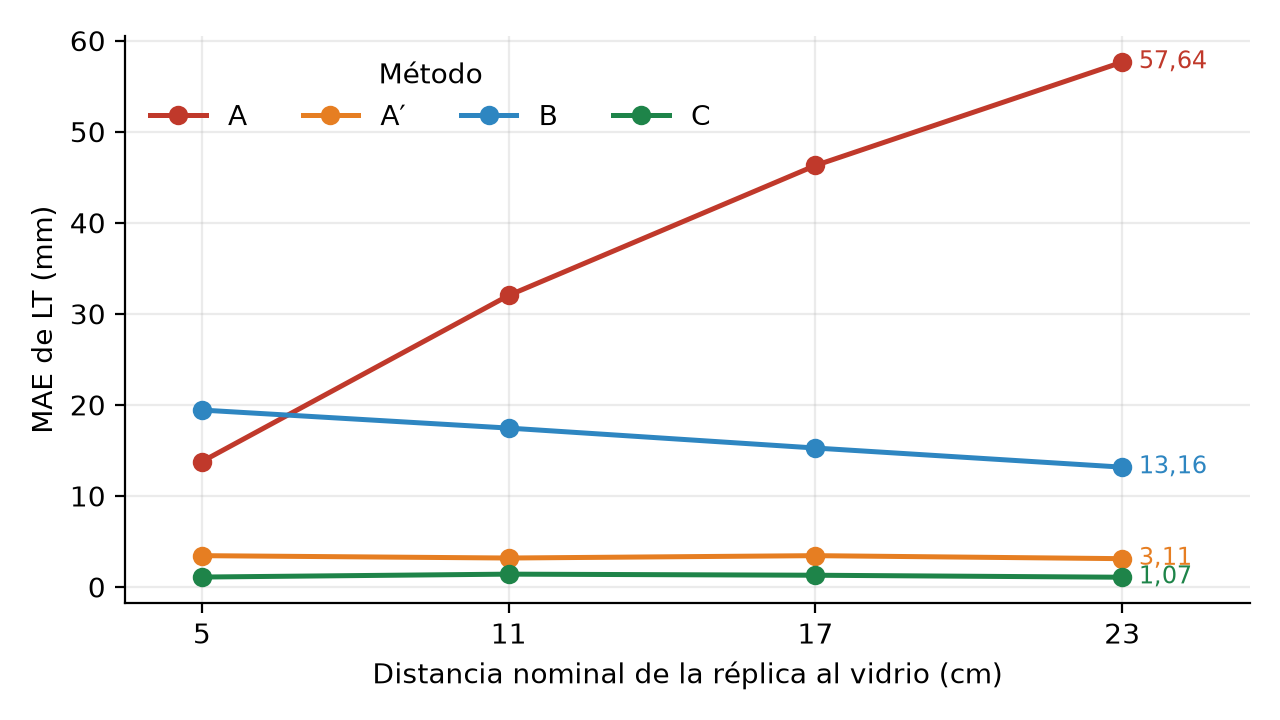
\includegraphics{figuras/fig4_2_mae_lt_profundidad.png}
\caption[MAE de longitud total por método y profundidad]{Error absoluto medio de longitud total por método y distancia de la réplica al vidrio (datos de la Tabla~\ref{tab:posiciones-mae}). El error de A crece con la profundidad; el de B disminuye levemente; \Aprime{} y C se mantienen estables. Fuente: elaboración propia.}
\label{fig:4-2}
\end{figure}

El error de A aumentó de 13,77~mm a 5~cm hasta 57,64~mm a 23~cm, con una pendiente de 2,43~mm por centímetro de separación. Este comportamiento es compatible con una escala calculada en el plano del vidrio: al alejarse la réplica, la misma escala deja de representar adecuadamente su plano de medición. La predicción de primer orden de la ecuación~\eqref{eq:Dz} para una réplica de 140~mm da errores de $-19$, $-37$, $-50$ y $-60$~mm en las cuatro posiciones, frente a los $-14$, $-32$, $-46$ y $-58$~mm observados; la diferencia máxima, de 6~mm, es atribuible a que $d$ se midió desde el frente de la lente y a que las réplicas tienen longitudes distintas. Esta coincidencia es una verificación independiente del modelo óptico: el error de A es el que la geometría predice.

\Aprime{} se mantuvo cerca de 3,1--3,5~mm en todas las posiciones, lo que indica que el marcador coplanar redujo la variación asociada a la perspectiva. B mostró una reducción del MAE de 19,43 a 13,16~mm, pero conservó un sesgo positivo; la diferencia B $-$ C disminuyó de 18,34 a 12,09~mm, con una pendiente de $-0{,}35$~mm por centímetro de separación. C permaneció entre 1,07 y 1,41~mm, sin una tendencia monótona con la profundidad.

Para PC se observó un patrón equivalente para A: el MAE pasó de 3,02~mm a 5~cm a 14,24~mm a 23~cm. \Aprime{} varió entre 0,75 y 1,34~mm, B entre 2,77 y 4,54~mm y C entre 0,48 y 0,62~mm. \pend{Si las referencias de PC de R1 y R2 cambian al volver a medirlas, actualizar estas cifras.}

\pendiente{Agregar, a partir del CSV maestro, una figura con el error con signo de cada una de las 24 combinaciones réplica--profundidad por método (puntos individuales, no promedios), para mostrar la dispersión además de la media.}

\section{Repetibilidad del marcado manual}
\label{sec:repetibilidad}

\pendiente{Volver a marcar los cuatro puntos en doce imágenes (una por réplica a 5 y a 23~cm) sin consultar el marcado anterior, y completar la Tabla~\ref{tab:repetibilidad} con la diferencia media y máxima en píxeles por punto y su efecto en milímetros sobre LT y PC calculado con C. Cerrar con: «La repetibilidad del marcado introduce una variación de X~mm en LT, inferior/comparable al MAE de C y muy inferior a la diferencia entre métodos, por lo que las conclusiones de las Secciones~\ref{sec:agregados} y~\ref{sec:profundidad} no dependen del operador».}

\begin{table}[htbp]

\caption{Repetibilidad del marcado manual sobre doce imágenes remarcadas.}
\label{tab:repetibilidad}
\begin{tabular}{@{}p{3cm}p{2cm}p{2.2cm}p{3.2cm}p{1.6cm}@{}}
\hline
Punto & Diferencia media (px) & Diferencia máxima (px) & Efecto medio en la medida (mm, con C) & Medida afectada \\
\hline
$\mathbf{p}_1$ (hocico) & \pend{ } & \pend{ } & \pend{ } & LT \\
$\mathbf{p}_2$ (extremo caudal) & \pend{ } & \pend{ } & \pend{ } & LT \\
$\mathbf{p}_3$ (perfil dorsal) & \pend{ } & \pend{ } & \pend{ } & PC \\
$\mathbf{p}_4$ (perfil ventral) & \pend{ } & \pend{ } & \pend{ } & PC \\
\hline
\end{tabular}
\end{table}

\section{Intervalo por profundidad desconocida}
\label{sec:intervalo}

La pregunta principal de este trabajo es qué intervalo de longitud puede garantizar C cuando la profundidad $z$ es desconocida y en qué condiciones ese intervalo es utilizable. Con el modelo de puerto plano, la longitud estimada para una misma imagen es una función $L(z)$ de la profundidad asumida; el intervalo $\IL$ de la ecuación~\eqref{eq:IL} recoge su variación sobre el rango admisible.

Para incidencia cercana a la normal, la magnificación de un punto situado a profundidad $z$ detrás del vidrio es, en primer orden, proporcional a $1/D(z)$, con $D(z) = d + t_g/\mu_g + z/\mu_w$ (ecuación~\ref{eq:Dz}), donde $d = 230$~mm, $t_g = 4$~mm, $\mu_g = 1{,}5$ y $\mu_w = 1{,}333$. Por tanto, $L(z)$ es proporcional a $D(z)$, creciente en $z$, y el intervalo puede escribirse como $[L(z_{\min}), L(z_{\max})]$. Esta misma relación reproduce el error observado de A dentro de 6~mm (Sección~\ref{sec:profundidad}), lo que respalda su uso para el intervalo.

Con ella, el ancho relativo de $\IL$ para una réplica situada a profundidad real $z_0$ es $(D(z_{\max}) - D(z_{\min}))/D(z_0)$. La Tabla~\ref{tab:intervalo} y la Figura~\ref{fig:4-3} presentan ese ancho para las cuatro posiciones y tres escenarios de conocimiento de $z$: desconocida en toda la pecera (0--30~cm), conocida con $\pm 3$~cm y conocida con $\pm 1$~cm.

\begin{table}[htbp]

\caption{Ancho relativo del intervalo $\IL$ (\% de LT) según la profundidad real de la réplica y el conocimiento disponible sobre $z$ (predicción geométrica de primer orden).}
\label{tab:intervalo}
\begin{tabular}{@{}lcccc@{}}
\hline
Conocimiento de $z$ & 5~cm & 11~cm & 17~cm & 23~cm \\
\hline
Desconocida en toda la pecera (0--30~cm) & 83 & 71 & 63 & 56 \\
Conocida con $\pm 3$~cm & 17 & 14 & 13 & 11 \\
Conocida con $\pm 1$~cm & 6 & 5 & 4 & 4 \\
\hline
Referencia: MAPE de \Aprime{} con $z$ conocida & \multicolumn{4}{c}{2,3} \\
Referencia: MAPE de C con $z$ conocida & \multicolumn{4}{c}{0,9} \\
\hline
\end{tabular}
\end{table}

\begin{figure}[htbp]
\centering
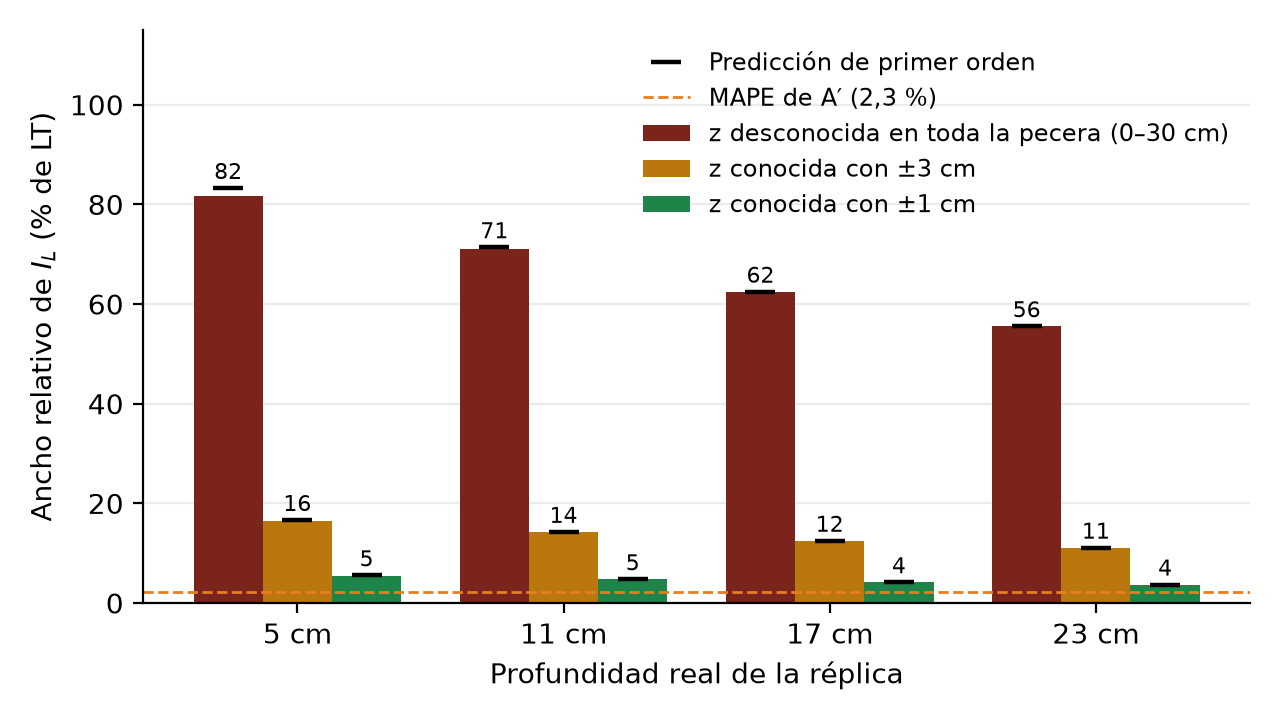
\includegraphics{figuras/fig4_3_ancho_intervalo.png}
\caption[Ancho relativo del intervalo por profundidad desconocida]{Ancho relativo del intervalo $\IL$ según la profundidad real de la réplica y el conocimiento disponible sobre $z$ (datos de la Tabla~\ref{tab:intervalo}). La línea discontinua marca el MAPE de \Aprime{} con profundidad conocida. Fuente: elaboración propia.}
\label{fig:4-3}
\end{figure}

Con una sola cámara y sin información de profundidad, el intervalo abarca entre 56 y 83~\% de la longitud de la réplica: no es utilizable para morfometría. Si la profundidad se acota a $\pm 3$~cm (por ejemplo, con una guía o un tanque angosto), el ancho baja a 11--17~\%, todavía mayor que el error de cualquiera de los métodos con $z$ conocida. Solo cuando la profundidad se conoce con $\pm 1$~cm el ancho (4--6~\%) se vuelve comparable con el error de \Aprime{} (2,3~\%) y queda dentro de un orden de magnitud del de C (0,9~\%). Este es el resultado que responde la pregunta principal: el modelo refractivo elimina el error de conversión, pero la profundidad sigue siendo la fuente dominante de incertidumbre y debe medirse o acotarse, no asumirse.

\pendiente{Ejecutar \texttt{measure\_c} sobre las 72 imágenes con el plano de medición en $z = 0, 10, 20, \ldots, 300$~mm, guardar $L(z)$ en \texttt{results/L\_z.csv} y (a) reemplazar los valores de la Tabla~\ref{tab:intervalo} por los numéricos, conservando los analíticos como columna de comparación; (b) reportar la cobertura empírica (fracción de las 72 capturas cuya LT de calibre cae dentro de $\IL$) para contrastar H3; (c) agregar una figura con $L(z)$ para dos imágenes de ejemplo, con la LT de calibre como línea horizontal y la $z$ real marcada, que verifica numéricamente la monotonía de $L(z)$.}

\section{Contraste de hipótesis}
\label{sec:contraste}

La Tabla~\ref{tab:hipotesis} resume el contraste de las tres hipótesis con los criterios fijados en la Sección~\ref{sec:evaluacion}.

\begin{table}[htbp]

\caption{Contraste de hipótesis.}
\label{tab:hipotesis}
\begin{tabular}{@{}p{1.2cm} X X p{2.3cm}@{}}
\hline
Hipótesis & Criterio & Valor observado & Veredicto \\
\hline
H1 & Prueba de signos exacta por réplica, $p < 0{,}05$, para C frente a A, \Aprime{} y B en LT & C mejor en 6 de 6 réplicas frente a cada método ($p = 0{,}031$); 24 de 24 combinaciones (descriptivo) & Se sostiene \\
H2 & Pendiente positiva de $\mathrm{MAE}_B - \mathrm{MAE}_C$ frente a la separación & Pendiente $-0{,}35$~mm/cm (18,3; 16,0; 14,0; 12,1~mm) & No se sostiene \\
H3 & Cobertura $\geq 0{,}95$ y ancho predicho dentro de la mitad del observado & Ancho predicho: 56--83~\% (toda la pecera); cobertura empírica \pend{pendiente} & \pend{Parcial: ancho predicho; cobertura no evaluada} \\
\hline
\end{tabular}
\end{table}

\paragraph{H1 se sostiene.} C tuvo menor error absoluto de LT que A, \Aprime{} y B en las seis réplicas (prueba de signos exacta con la réplica como unidad, $p = 0{,}031$ en cada comparación) y en las 24 combinaciones réplica--profundidad (descriptivo); en PC fue mejor que A y B en 24 de 24 combinaciones y que \Aprime{} en 21 de 24. La parte de H1 que, en el protocolo, preveía equivalencia entre B y C dentro de la zona de calibración no se evaluó formalmente porque el margen $\delta$ no se fijó antes de observar los datos; la diferencia observada a 5~cm fue de 19,43~mm (B) frente a 1,09~mm (C), de modo que, aun sin prueba de equivalencia, los datos no respaldan que B y C sean intercambiables en esa zona.

\paragraph{H2 no se sostiene.} La diferencia B $-$ C disminuyó con la separación (18,34; 16,04; 13,96 y 12,09~mm; pendiente $-0{,}35$~mm/cm). El sesgo positivo y casi constante de B ($+16{,}3$~mm en promedio) indica un error sistemático de escala del plano de referencia de B, y no la degradación con la distancia descrita por \textcite{Rofallski2022}; la interpretación se desarrolla en la Sección~\ref{sec:discusion}. Este resultado no debilita la conclusión principal: con o sin ese sesgo, C fue el método de menor error en las cuatro posiciones.

\paragraph{H3 se sostiene parcialmente.} El ancho del intervalo es predecible a partir de la geometría del montaje, y la misma predicción reproduce el error de A dentro de 6~mm. La cobertura empírica sobre las 72 capturas no se evaluó en esta versión; su cálculo requiere la corrida de $L(z)$ descrita en la Sección~\ref{sec:intervalo} y queda declarado como verificación inmediata. \pend{Actualizar el veredicto cuando se disponga de la cobertura.}

\section{Discusión de los resultados}
\label{sec:discusion}

La comparación se realizó sobre los mismos puntos anatómicos y las mismas imágenes, por lo que la diferencia observada se relaciona principalmente con la transformación geométrica de cada ruta. La escala de A utiliza una referencia fija en el vidrio y no compensa la separación entre ese plano y el pez; el aumento de su error con la profundidad es el resultado más claro del conjunto y coincide con la predicción de primer orden del modelo óptico. \Aprime{} reduce ese efecto al trasladar la referencia al plano aproximado de la réplica, aunque sigue dependiendo de la calidad del marcado y de la coplanaridad conseguida. Conviene precisar la atribución causal: la diferencia entre A y \Aprime{} incluye tanto la coplanaridad del marcador como la rectificación por homografía, y la ventaja de C incluye el modelo completo de interfaces y la información de profundidad, no «la refracción» como causa única.

B presentó un sesgo positivo casi constante ($+16{,}3$~mm en promedio) y un MAE que disminuyó levemente con la distancia. Este patrón no corresponde a la degradación con la separación de la zona de calibración prevista por \textcite{Rofallski2022}, sino a un error sistemático de escala: la calibración bajo agua compensó la refracción en el rango cubierto (la razón de focales de 1,36 lo muestra), pero el plano de referencia obtenido del riel (Tabla~\ref{tab:riel}, con un error relativo de escala informado de 0,813~\%) o la distancia nominal del carrito introducen una sobreestimación común a todas las posiciones. Un error de escala constante es corregible con una medida patrón, mientras que el error de A no lo es porque depende de $z$. La verificación de la referencia del riel y de la distancia de calibración queda como trabajo inmediato.

C obtuvo los errores medios más bajos porque incorpora las interfaces aire--vidrio--agua y evalúa la geometría en cada profundidad. Tres evidencias respaldan que ese resultado no es casual: la prueba de sanidad del módulo (con $\mu = 1$ y $t_g = 0$ reproduce la cámara pinhole), el error de 0,88~\% contra calibre en 72 imágenes y cuatro profundidades, y la coincidencia entre la predicción geométrica del error de A y lo observado. La ventaja de C se sostiene contra referencias físicas independientes del software (calibre) en 24 combinaciones; la comprobación complementaria con barra patrón, que permitiría separar un eventual error de implementación del error de marcado, queda pendiente.

Como comprobación de sensibilidad frente a la advertencia de unidad en las referencias de PC de R1 y R2, al considerar solo R3--R6 se conserva el mismo orden de MAE de PC: C (0,62~mm), \Aprime{} (1,04~mm), B (3,60~mm) y A (9,03~mm). Por tanto, esa advertencia modifica la precisión de las cifras de PC, pero no cambia la interpretación cualitativa.

Frente a los antecedentes, el error de C con profundidad conocida (MAE 1,22~mm; 0,88~\%) es menor que el informado por MorphoCal (MAE 7,5~mm, cámara sumergida y peces vivos; \citeauthor{Vijayalakshmi2026}, \citeyear{Vijayalakshmi2026}) y por \textcite{Seibold2026} (RMSE 6--9~mm, estéreo y peces vivos), pero las condiciones no son equivalentes: este trabajo usó réplicas rígidas, posturas controladas, puntos marcados a mano y una profundidad conocida por el soporte. La comparación válida no es entre cifras sino entre preguntas: los sistemas estéreo resuelven la profundidad con la segunda cámara; aquí se cuantificó qué se pierde al no tenerla.

\pendiente{Agregar la figura de Bland--Altman de C frente al calibre (diferencia frente a promedio, con sesgo y límites de acuerdo) y una figura con una captura real (por ejemplo R3 a 23~cm) con los cuatro puntos marcados y, al pie, las cuatro estimaciones y la referencia. Ambas requieren el CSV maestro y las imágenes.}

\section{Alcance de los resultados}

Los resultados son válidos para las seis réplicas rígidas, la cámara Realme C71, la pecera de vidrio, las cuatro posiciones y las condiciones de iluminación utilizadas. No se generalizan directamente a peces vivos, movimiento, turbidez, oclusiones ni posiciones laterales que no fueron incluidas en la captura. Del mismo modo, las tres capturas técnicas no deben interpretarse como tres unidades experimentales independientes, y las 24 combinaciones réplica--profundidad no son 24 unidades: la unidad experimental es la réplica ($n = 6$).

En conjunto, los datos respaldan una ventaja de C y, en segundo lugar, de \Aprime{} frente a A y B para las medidas analizadas, con la réplica como unidad y contra referencias físicas de calibre. La conclusión se limita al flujo de procesamiento, al montaje y a las referencias físicas registradas.

\chapter{Conclusiones y recomendaciones}
\label{cap:conclusiones}

El trabajo permitió evaluar, dentro de un montaje controlado aire--vidrio--agua, cuatro rutas de conversión métrica aplicadas a las mismas imágenes y a los mismos puntos anatómicos, y cuantificar el intervalo de longitud que induce una profundidad desconocida. El conjunto analizado estuvo formado por seis réplicas rígidas de PLA, cuatro profundidades, tres capturas técnicas por condición y 72 imágenes. Las conclusiones que siguen se refieren a este conjunto y a las referencias físicas registradas en el CSV maestro.

El aporte del trabajo se resume en una regla de decisión (Tabla~\ref{tab:regla} y Figura~\ref{fig:5-1}): qué conversión usar según lo que se sabe de la escena, con el error esperado en este montaje.

\begin{table}[htbp]

\caption{Regla de decisión: qué conversión usar según la situación, con el error observado en este montaje.}
\label{tab:regla}
\begin{tabular}{@{}X p{2.6cm} p{3.0cm} X@{}}
\hline
Situación de uso & Método recomendado & Error esperado en este montaje & Condición \\
\hline
Se puede poner un marcador junto al pez, en su mismo plano & \Aprime{} (homografía con marcador coplanar) & $\approx$ 2--3~\% de LT (3,3~mm) & Coplanaridad dentro de $\pm 1$~cm; no requiere calibración \\
No se puede poner un marcador junto al pez, pero se conoce su distancia al vidrio (riel, guía, tanque angosto) & C (puerto plano) & $< 1$~\% de LT (1,2~mm) & Calibración en aire y parámetros $d$, $t_g$ e índices del puerto \\
Solo hay calibración bajo agua y el pez está en la zona calibrada & B (pinhole efectivo) & $\approx$ 10~\% con sesgo constante en este montaje; corregible con un patrón & Verificar la escala del plano de referencia \\
Marcador fijo en el vidrio y pez a distancia desconocida & Ninguno es aceptable (A) & 10--40~\% según la distancia & Solo sirve si el pez está pegado al vidrio \\
No se sabe nada de la profundidad & C con intervalo $\IL$ & 56--83~\% de ancho: no utilizable & Hay que acotar $z$; con $\pm 1$~cm el ancho baja a 4--6~\% \\
\hline
\end{tabular}
\end{table}

\begin{figure}[htbp]
\centering
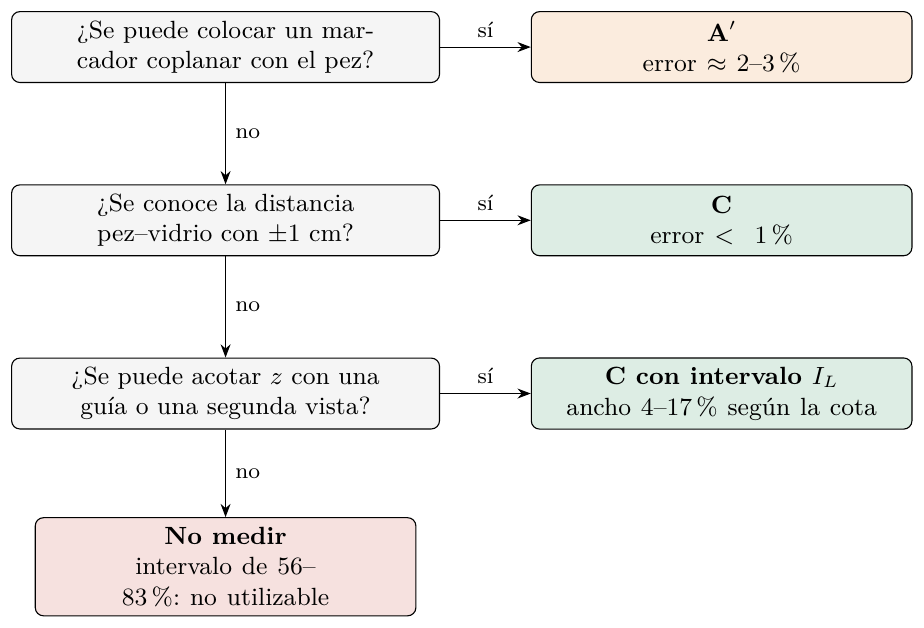
\includegraphics[width=\textwidth]{figuras/tikz/tikz_5.png}
\caption[Diagrama de decisión para la conversión métrica monocular a través de un vidrio plano]{Diagrama de decisión para la conversión métrica monocular a través de un vidrio plano. Cada hoja indica el error observado en este montaje (Capítulo~\ref{cap:resultados}). Fuente: elaboración propia.}
\label{fig:5-1}
\end{figure}

\section{Conclusiones por objetivo}
\label{sec:conclusiones}

\begin{enumerate}
  \item \textbf{Conjunto de datos (objetivo 1).} Se construyó y documentó un conjunto de 72 imágenes de seis réplicas a cuatro profundidades, con referencias físicas de calibre, tabla maestra trazable por réplica, profundidad, repetición e imagen, y registro de exclusiones: se obtuvieron valores numéricos para 284 de los 288 registros y los cuatro restantes correspondieron a A y \Aprime{} en dos imágenes sin detección del marcador. Las repeticiones técnicas se resumieron por combinación réplica--profundidad. Objetivo cumplido.
  \item \textbf{Protocolo y repetibilidad del marcado (objetivo 2).} Se estableció y aplicó un protocolo de marcado manual único por imagen, con cuatro puntos definidos anatómicamente y reutilizados por las cuatro rutas. La repetibilidad del marcado \pend{se cuantificó en la Sección~\ref{sec:repetibilidad} con una variación de X~mm en LT / no se cuantificó en esta versión y queda como verificación inmediata}. Objetivo \pend{cumplido / cumplido parcialmente}.
  \item \textbf{Implementación y validación de las rutas (objetivo 3).} Las cuatro rutas se implementaron en una aplicación propia de código abierto, con pruebas unitarias de sanidad para el módulo de puerto plano, y se evaluaron contra las referencias de calibre de las seis réplicas en 72 imágenes. C alcanzó un MAE de 1,22~mm (0,88~\%) en LT y 0,56~mm (1,62~\%) en PC; \Aprime{} obtuvo 3,29~mm (2,28~\%) y 1,03~mm (2,78~\%). La comprobación instrumental con barra patrón no se realizó. Objetivo cumplido en su validación contra referencias físicas; comprobación con patrón pendiente.
  \item \textbf{Comparación pareada según la separación (objetivo 4).} A mostró la mayor sensibilidad a la profundidad: su MAE de LT aumentó de 13,77~mm a 5~cm hasta 57,64~mm a 23~cm (2,43~mm por centímetro), como predice la geometría del puerto plano. B mantuvo un sesgo positivo casi constante y C se mantuvo entre 1,07 y 1,41~mm en las cuatro posiciones. C tuvo menor error que cada otro método en 6 de 6 réplicas ($p = 0{,}031$) y en 24 de 24 combinaciones. H1 se sostiene; H2 no se sostiene, y el comportamiento de B se interpreta como un error de escala del plano de referencia y no como degradación con la distancia. Objetivo cumplido.
  \item \textbf{Intervalo por profundidad desconocida (objetivo 5).} El intervalo $\IL$ se calculó a partir de la geometría del montaje, verificada contra el error observado de A: su ancho es de 56--83~\% de LT si $z$ se desconoce en toda la pecera, de 11--17~\% con $\pm 3$~cm y de 4--6~\% con $\pm 1$~cm. La cobertura empírica sobre las 72 capturas \pend{no se evaluó en esta versión / fue de X}. Objetivo \pend{cumplido parcialmente: ancho sí, cobertura pendiente}.
  \item \textbf{Sensibilidad (objetivo 6).} La sensibilidad de C a la distancia cámara--vidrio y al índice del agua \pend{se cuantificó en la Tabla~\ref{tab:sensibilidad} / se acotó analíticamente (un error de 10~mm en $d$ corresponde a 2,5--3,7~\% de LT) y queda pendiente su cálculo numérico}. Objetivo \pend{cumplido / cumplido parcialmente}.
\end{enumerate}

La Tabla~\ref{tab:cumplimiento} resume el grado de cumplimiento de cada objetivo.

\begin{table}[htbp]

\caption{Matriz de cumplimiento de los objetivos específicos.}
\label{tab:cumplimiento}
\begin{tabular}{@{}p{1.4cm} X p{1.8cm} X@{}}
\hline
Objetivo & Resultado que lo sostiene & Grado & Pendiente \\
\hline
1 & Tablas~\ref{tab:replicas} y~\ref{tab:registros}; repositorio & Cumplido & Publicar los datos con la etiqueta \texttt{\RepoTag} \\
2 & Sección~\ref{sec:procedimiento}; Tabla~\ref{tab:repetibilidad} & \pend{Parcial} & Remarcado de doce imágenes \\
3 & Tablas~\ref{tab:calibraciones} y~\ref{tab:agregados} & Cumplido & Comprobación con barra patrón \\
4 & Tabla~\ref{tab:posiciones-mae}; Tabla~\ref{tab:hipotesis} & Cumplido & Verificar el plano de referencia de B \\
5 & Tabla~\ref{tab:intervalo}; Figura~\ref{fig:4-3} & \pend{Parcial} & Corrida de $L(z)$ y cobertura empírica \\
6 & Tabla~\ref{tab:sensibilidad} & \pend{Parcial} & Ejecución de \texttt{sensitivity\_c()} \\
\hline
\end{tabular}
\end{table}

En síntesis: a través de un vidrio plano, la escala de un marcador fijo no sirve para medir un pez a otra profundidad, porque el error crece 2,4~mm por cada centímetro de separación. Un marcador en el plano del pez reduce ese error a 2--3~\%, y el modelo refractivo de puerto plano a menos del 1~\% cuando la profundidad se conoce. Cuando no se conoce, la geometría acota la longitud a un intervalo demasiado ancho para morfometría, salvo que la profundidad se restrinja a $\pm 1$~cm. Por tanto, en un sistema monocular la profundidad, no la refracción, es la fuente de incertidumbre que hay que resolver, y este trabajo cuantifica cuánto.

\section{Limitaciones}

El estudio se realizó con réplicas rígidas, una cámara monocular y una pecera de vidrio en condiciones de iluminación y encuadre controlados. No se evaluaron peces vivos, movimiento, turbidez, oclusiones ni posiciones laterales planificadas. La muestra, no probabilística y de seis réplicas, no permite generalizar los resultados a otras especies, tamaños, cámaras o configuraciones de puerto; las conclusiones son relativas a este montaje.

La inferencia se realizó con una prueba de signos exacta sobre diferencias pareadas por réplica; no se aplicaron pruebas paramétricas porque $n = 6$ réplicas no permite verificar sus supuestos, y los conteos sobre 24 combinaciones son descriptivos. La comprobación instrumental con una barra patrón sumergida no se realizó; la validación métrica es la comparación con las referencias de calibre. La cobertura empírica del intervalo $\IL$ y la repetibilidad del marcado \pend{no se cuantificaron en esta versión}, por lo que los objetivos 2, 5 y 6 se declaran parcialmente cumplidos.

\section{Recomendaciones}

Para repetir el procedimiento se recomienda conservar la cámara, resolución, enfoque, iluminación, posición de la pecera y configuración del puerto durante todo el conjunto de capturas. También deben conservarse la imagen original, los puntos manuales, los archivos de calibración, la versión del programa y el registro de exclusiones. Se recomienda registrar una medida física sumergida independiente (barra patrón) para cada sesión y repetir la evaluación con posiciones laterales del encuadre.

Para el uso práctico, la Tabla~\ref{tab:regla} resume la recomendación: la escala A debe interpretarse solo como una línea base, no como una corrección refractiva; B debe utilizarse dentro de la zona para la que se calibró y con su escala verificada contra un patrón; C debe conservar los parámetros físicos del puerto, los índices de refracción y el sistema de coordenadas documentados, y requiere conocer o acotar la profundidad para que su salida sea utilizable.

\section{Trabajos futuros}

\paragraph{Verificaciones inmediatas sobre este mismo conjunto.} Corrida de $L(z)$ sobre las 72 imágenes para obtener la cobertura empírica del intervalo y verificar numéricamente su monotonía; remarcado de doce imágenes para cuantificar la repetibilidad del operador; ejecución del análisis de sensibilidad a $d$ y $\mu_w$; nueva medición de las referencias de PC de R1 y R2; comprobación con una barra patrón sumergida; y revisión del plano de referencia del riel y de la distancia de calibración de B para confirmar el origen de su sesgo constante.

\paragraph{Líneas de continuación.} Detección automática de los puntos anatómicos sobre el mismo protocolo pareado, que permitiría medir el error de localización por separado del geométrico; estimación de la profundidad con una guía, una segunda vista o una restricción de postura, de modo que el intervalo $\IL$ se reduzca al rango utilizable; evaluación con peces vivos, turbidez y posiciones fuera del centro del encuadre; incorporación explícita de la incertidumbre de los parámetros del puerto y de los índices de refracción en el intervalo; y publicación del artículo derivado con el conjunto de datos y el código.

\section{Impacto potencial y aporte}

El principal aporte del trabajo es un procedimiento trazable para comparar conversiones métricas monoculares en un montaje aire--vidrio--agua, junto con la cuantificación de lo que puede afirmarse sobre la longitud cuando la profundidad no se conoce. La ruta C presenta el mejor desempeño en el conjunto analizado y \Aprime{} constituye una alternativa más simple con menor error que la escala fija en el vidrio.

Para la Ingeniería Informática el trabajo aporta: (1) un módulo de trazado refractivo de puerto plano implementado desde las formulaciones de \textcite{Agrawal2012} y \textcite{Treibitz2012}, con pruebas unitarias de sanidad (con $\mu_g = \mu_w = 1$ y $t_g = 0$ reproduce la cámara pinhole) y evaluado contra referencias físicas; (2) una aplicación de escritorio de código abierto que mantiene la trazabilidad por imagen (puntos, calibración, versión y advertencias) y exporta un registro reproducible; (3) un procedimiento experimental pareado que aísla el efecto del modelo geométrico y que puede reutilizarse para evaluar detectores automáticos de puntos; y (4) evidencia cuantitativa sobre cuándo basta un marcador, cuándo una calibración bajo agua y cuándo se necesita el modelo físico, en este montaje.

Para la acuicultura, el resultado es una regla práctica con números para medir peces sin sacarlos del agua con una cámara común a través del vidrio de un tanque. La aplicación sobre peces vivos o en instalaciones productivas debe considerarse una posibilidad futura hasta completar la validación en esas condiciones.

\chapter*{Referencias}
\appendix
\chapter{Registro visual de capturas}
\label{anx:capturas}

La Figura~\ref{fig:A-1} presenta una vista conjunta de las capturas utilizadas en el flujo de trabajo. Las etiquetas visibles siguen el patrón de identificación de la réplica, la repetición y la posición nominal del riel en milímetros, por ejemplo \texttt{R1-REP1-50.jpg}. La imagen permite comprobar la organización visual del conjunto y la correspondencia entre las posiciones de captura. Las 72 imágenes originales forman parte del repositorio (Anexo~\ref{anx:repositorio}).

\begin{figure}[htbp]
\centering
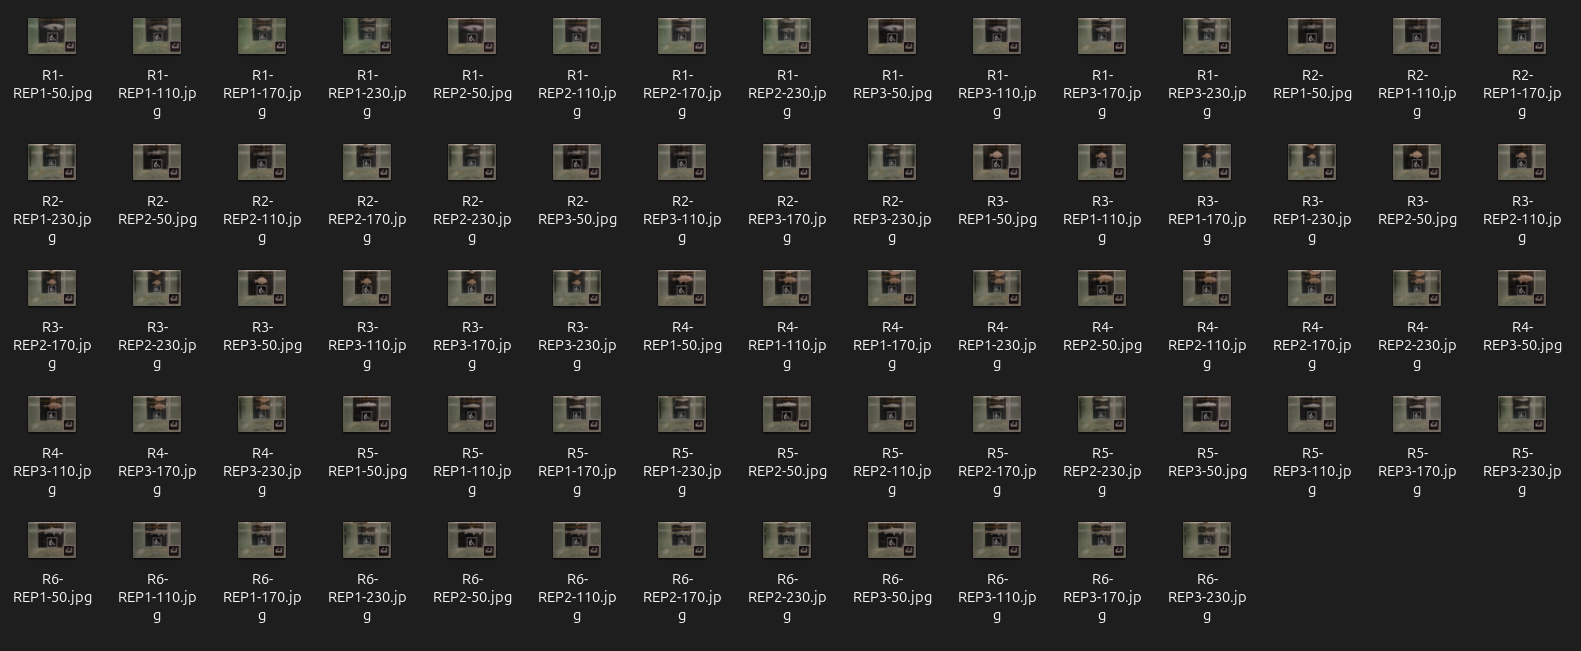
\includegraphics{figuras/originales/figA_1_capturas.png}
\caption[Vista conjunta de las capturas y sus identificadores]{Vista conjunta de las capturas y sus identificadores. Fuente: elaboración propia.}
\label{fig:A-1}
\end{figure}

\chapter{Configuración del puerto plano}
\label{anx:flatport}

La Figura~\ref{fig:B-1} reproduce la configuración utilizada para el modelo del puerto plano, cuyos valores se resumen en la Tabla~\ref{tab:puerto}: unidades en milímetros, normal de cámara $(0, 0, 1)$, distancia de la interfaz de 230~mm, espesor del vidrio de 4~mm e índices de refracción de 1,000 para aire, 1,500 para vidrio y 1,333 para agua. También registra que la distancia de la lente es una aproximación medida desde el frente de la lente y que las condiciones del agua corresponden a 22~\si{\celsius}, salinidad 0 y presión 0~dbar.

\begin{figure}[htbp]
\centering
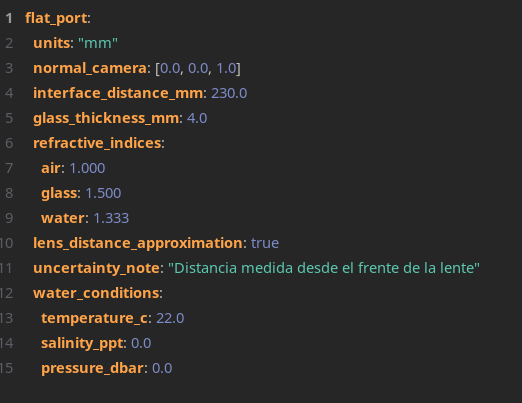
\includegraphics{figuras/originales/figB_1_flatport.png}
\caption[Parámetros visibles de la configuración del puerto plano]{Parámetros visibles de la configuración del puerto plano. Fuente: Fishmeter.}
\label{fig:B-1}
\end{figure}

\chapter{Parámetros de calibración de cámara}
\label{anx:calibraciones}

Los archivos \texttt{calibration\_B.yaml} y \texttt{calibration\_C\_air.yaml} contienen los perfiles de calibración utilizados por las rutas B y C. Ambos emplean el modelo de cámara de OpenCV, una resolución de $4096 \times 3072$ píxeles y un tablero con $4 \times 4$ esquinas interiores y cuadros de 20~mm. Sus indicadores de calidad se presentan en la Tabla~\ref{tab:calibraciones}. Los siguientes listados reproducen la cabecera y los campos de resumen de cada archivo; los informes individuales de las vistas permanecen en los YAML completos del repositorio.

\begin{lstlisting}[caption={Cabecera y resumen del perfil B.},label={lst:calB}]
schema: fish_morphometry.b_calibration.v1
profile_id: B-effective
profile_hash: eb245104cb46caded48e9e9f827dda11db985c7b22ec5cb63a27572da14caf4e
calibration_context_hash: 1e3531dcf0d9ff8d00b322b41d2dd074b41cb822a1324cd5545635303ca81ba6
model: OPENCV
camera_matrix:
- [4502.32284117, 0.0, 2027.2736574393155]
- [0.0, 4504.395746404586, 1549.0026630316365]
- [0.0, 0.0, 1.0]
distortion_coefficients:
- 0.4454686711747631
- -3.4668133596510753
- -0.008336348094703296
- 0.004790603340447537
- 8.25240238252019
resolution: [4096, 3072]
calibration_rail_position_mm: 0.0
created_at_utc: '2026-10-12T04:07:10.722788+00:00'
versions:
  opencv: 5.0.0
  fish_morphometry: 0.1.0
source: opencv_calibrateCamera
board:
  inner_corners: [4, 4]
  square_size_mm: 20.0
rms_px: 0.4353568098178903
views:
  received: 35
  accepted: 35
  rejected: 0
\end{lstlisting}

\begin{lstlisting}[caption={Cabecera y resumen del perfil C en aire.},label={lst:calC}]
schema: fish_morphometry.air_calibration.v1
profile_id: C-air
profile_hash: fb98aea6af6ba57d663f5884b4034bfff3413c62cc376bef82256a7c1f412a55
calibration_context_hash: 623631f83c66f4b1615fd73e2f4db719880ccaa11c117bc705674d1a0df96ef8
model: OPENCV
camera_matrix:
- [3313.72125140631, 0.0, 2028.1975106019397]
- [0.0, 3313.6744263215105, 1530.5739559303083]
- [0.0, 0.0, 1.0]
distortion_coefficients:
- 0.18564347583186028
- -0.829350911254369
- -0.0011635185172718578
- -0.0015902497923188043
- 1.0012733784385703
resolution: [4096, 3072]
board:
  inner_corners: [4, 4]
  square_size_mm: 20.0
  units: mm
rms_px: 0.3745461951579489
created_at_utc: '2026-10-12T04:12:38.034127+00:00'
versions:
  opencv: 5.0.0
  fish_morphometry: 0.1.0
source: opencv_calibrateCamera_air
views:
  received: 36
  accepted: 36
  rejected: 0
\end{lstlisting}

\chapter{Referencia geométrica del riel para B}
\label{anx:riel}

El archivo \texttt{rail\_reference\_B.yaml} documenta el plano de referencia utilizado por B. El plano se obtuvo a partir de dos posiciones del riel, 0 y 180~mm, con un umbral de reproyección de 1,0~px. El ajuste informa un residuo lineal de $1{,}62 \times 10^{-13}$~mm (residuo numérico de una recta por dos puntos, que no representa la incertidumbre física), una dispersión máxima de la normal de $1{,}0^{\circ}$ y un error relativo de escala de 0,813~\%. El archivo también registra que los planos de las réplicas se consideran paralelos al tablero, mientras que el riel no se considera perpendicular al tablero. Los valores principales se resumen en la Tabla~\ref{tab:riel}.

\begin{lstlisting}[caption={Cabecera y plano de referencia del riel para B.},label={lst:riel}]
plane_point_camera_mm:
- -34.117491789288806
- -28.291160700295567
- 365.1469994117171
plane_normal_camera:
- -0.03972877728543376
- -0.042783728187314775
- 0.9982941334385363
z_ref_mm: 0.0
rail_direction_camera:
- 0.02095849070805215
- -0.04478647483729878
- 0.998776708448334
\end{lstlisting}

\chapter{Repositorio de código y datos}
\label{anx:repositorio}

El código de la aplicación, los datos del experimento y los scripts que regeneran las tablas y figuras del Capítulo~\ref{cap:resultados} se encuentran en \url{\RepoURL}, etiqueta \texttt{\RepoTag}. Hash completo del commit de referencia:\par\noindent{\footnotesize\texttt{\RepoCommit}}\par La estructura del repositorio es la siguiente:

\begin{lstlisting}
FishmeterTPF/
  src/fish_morphometry/   aplicacion Fishmeter (calibracion, geometria,
                          metodos A, A', B y C, interfaz, validacion)
  tests/                  pruebas unitarias e integracion (pytest)
  calibrations/           air/, water_pinhole/, flatport/ (YAML)
  data/raw/               72 imagenes JPG originales
  data/annotations/       puntos anatomicos (JSON por imagen)
  data/references/        replicas.csv (medidas de calibre x3)
  results/master.csv      tabla maestra (288 registros)
  results/L_z.csv         L(z) por imagen (grilla de profundidades)
  analysis/make_figures.py  regenera tablas y figuras del Capitulo 4
  docs/                   guia de uso y notas de desarrollo
  README.md               instalacion, ejecucion y reproduccion
\end{lstlisting}

\pendiente{Publicar en el repositorio las 72 imágenes, los JSON de puntos, \texttt{replicas.csv}, los tres YAML, \texttt{master.csv} y \texttt{L\_z.csv}; mover las notas internas de desarrollo a \texttt{docs/dev/}; agregar \texttt{requirements.txt} congelado; crear la etiqueta \texttt{v1.0-tesis} y actualizar el hash en la Sección~\ref{sec:software} y en este anexo. Hasta entonces, no debe afirmarse que las tablas se reproducen desde el repositorio.}

\chapter{Tabla maestra de resultados}
\label{anx:maestra}

\pendiente{Incluir la tabla maestra (72 imágenes $\times$ 4 métodos: LT y PC estimadas y de referencia, error con signo y estado) en letra pequeña a dos columnas, o el enlace al CSV con su hash SHA-256.}

\chapter{Fichas de las réplicas}
\label{anx:fichas}

\pendiente{Incluir una ficha por réplica (R1--R6) con fotografía, origen del modelo STL, escala de impresión, material y las tres lecturas de calibre de LT y PC con su media y desviación.}

\chapter{Registro de cambios de esta versión}
\label{anx:cambios}

Esta versión del documento incorpora las observaciones de dos revisiones independientes realizadas el 13 de octubre de 2026 sobre la versión anterior del libro (77 páginas). El registro siguiente permite justificar cada cambio y lo que no se incorporó, conforme al artículo 17 del Reglamento de Proyecto Final. La numeración A-$n$ y B-$n$ remite a las correcciones de cada revisión.


\begin{longtable}{@{}p{1.6cm}p{2.0cm}p{6.0cm}p{5.0cm}@{}}
\caption{Registro de cambios respecto de la versión anterior.}
\label{tab:registro-cambios}\\
\hline
Ref. & Ubicación anterior & Cambio realizado & Motivo \\
\hline
\endfirsthead
\hline
Ref. & Ubicación anterior & Cambio realizado & Motivo \\
\hline
\endhead
\hline
\endfoot
\endlastfoot
A-1, B-26 & Cap.~1 y 2 & Los verbos en futuro que describían acciones realizadas pasaron a pretérito; las definiciones a presente; lo no realizado se declara como pendiente. & El documento informa una investigación concluida. \\
A-2, A-6, B-01 & Título, 1.5, 1.6, 4.6 & Se agregó la Sección~\ref{sec:intervalo} con la estimación geométrica del ancho de $\IL$ y su verificación contra el error de A; la corrida numérica y la cobertura quedan marcadas como pendientes. & El título y la pregunta principal prometían el intervalo y ninguna sección lo trataba. Se mantiene el título. \\
A-3, B-04/05 & 1.8, 4.4 & H1 y H2 reescritas con criterios coincidentes con lo calculado; nueva Sección~\ref{sec:contraste} con tabla de veredictos; H2 declarada no sostenida e interpretada. & No existía contraste de hipótesis; los datos refutaban H2 sin decirlo. \\
A-4, B-03 & 1.6, Cap.~4 & Secciones~\ref{sec:repetibilidad} y~\ref{sec:sensibilidad} creadas con sus tablas; matriz de cumplimiento en la Tabla~\ref{tab:cumplimiento}. & Objetivos 2, 5 y 6 sin resultado. \\
A-5, B-27 & pp.~8, 11, 19, 27, 30, 54, 62 & Eliminadas las frases de proceso («D7 del informe», «2-antecedente.tex», «carpeta anexo/», fila «pendiente de verificación»). & Texto dirigido al autor, no al lector. \\
A-7, B-12 & pp.~42--48 & Reemplazado «requiere comprobación física independiente / resultados exploratorios» por la descripción del estado interno del software y la validación contra calibre; distinción entre comprobación con patrón y validación externa. & La comparación contra calibre es la validación física. \\
A-8, B-07 & pp.~42--49 & Las cinco menciones a la advertencia de unidad de PC de R1 y R2 se concentraron en un recuadro pendiente de la Sección~\ref{sec:conjunto}. & Es una tarea de medición, no una limitación. \\
B-08 & 4.3 & La inferencia se hizo con la réplica como unidad (prueba de signos, $n = 6$, $p = 0{,}031$); los conteos 24/24 pasan a descriptivos. & Las 24 combinaciones son medidas repetidas de seis réplicas. \\
B-09, B-10 & 3.7, 4.1 & Se aclara que las métricas describen la estimación promedio por condición y que el pareamiento no es idéntico en dos combinaciones; recálculo con la intersección pendiente. & Rigor del diseño pareado. \\
A-9, B-23 & 3.3, Anexo E & Hash completo del commit y etiqueta prevista; Anexo~\ref{anx:repositorio} con el árbol del repositorio; publicación de datos pendiente. & Reproducibilidad. \\
A-10, B-15 & Cap.~3 & Tabla~\ref{tab:replicas} de réplicas y referencias (valores pendientes); lado físico de los ArUco pendiente. & El lector debe conocer contra qué se comparó. \\
A-11 & Cap.~4 & Figuras~\ref{fig:4-1}, \ref{fig:4-2} y~\ref{fig:4-3} generadas por script desde las tablas. & El capítulo no tenía figuras. \\
A-12, B-24 & Resumen & Resumen y abstract reescritos con hallazgos y conclusión (menos de 350 palabras), sin tareas pendientes. & Anexo I del reglamento. \\
A-13, B-18 & Cap.~1 & 1.2 ampliado; Sección~\ref{sec:conclusiones}; nueva 1.9.1 de delimitación; Tabla~\ref{tab:trazabilidad}. & Estructura del Anexo I y trazabilidad. \\
A-14, B-22 & Cap.~3 & 3.1 renombrada con tipo, enfoque, población y muestra; Tabla~\ref{tab:operacionalizacion}; Tablas~\ref{tab:puerto} y~\ref{tab:riel} subidas desde los anexos. & Marco metodológico del Anexo I. \\
A-15 & 4.5 & Párrafo sobre B reescrito: sesgo constante como error de escala, con la razón de focales 1,36. & Convertir una contradicción en un hallazgo interpretado. \\
A-16, B-43 & 5.5 & Párrafo con el aporte a la Ingeniería Informática; Tabla~\ref{tab:regla} y Figura~\ref{fig:5-1}. & Explicitar el aporte de la carrera. \\
A-17 & 5.4 & Trabajos futuros separados en verificaciones inmediatas y líneas de continuación. & Evitar leer el trabajo futuro como lista de incumplimientos. \\
A-18, B-28 & 2.7, Tabla 2.1 & Párrafo y filas de MorphoCal, Yin y Zhou con los datos verificados de las fuentes primarias. & Una fila «pendiente de verificación» es inadmisible en la versión final. \\
A-19, B-16/17 & 2.5, 3.4, 3.5 & Definición operacional de $\mathbf{p}_2$ y de LT; fórmula implementada de la escala (ecuación~\ref{eq:escala-impl}); homografía de \Aprime{} y plano de B formulados; nombres de funciones retirados del cuerpo. & Coherencia texto--código y rigor. \\
A-20, B-45 & 3.2 & Efecto de medir $d$ desde el frente de la lente acotado analíticamente; cálculo numérico pendiente. & Pregunta previsible de la mesa. \\
A-21 & 2.2 & Orden «aire--vidrio--agua» unificado en todo el documento. & Concordancia. \\
A-22 & 4.2 & Fórmulas definidas una sola vez en la Sección~\ref{sec:evaluacion}. & Concisión. \\
A-23 & 1.1 & Introducción reducida a tres párrafos; el estado del arte queda en 2.7. & Concisión. \\
A-24/25/26/27, B-38/39/41 & Preliminares & Orden según el Anexo I; numeración romana única; tildes; «Tutora: Ing. Evelyn Giménez»; «para optar al título de Ingeniero en Informática»; \texttt{hidelinks}. & Formato. \\
A-28 & Acrónimos & Lista reducida a las siglas usadas. & Rúbrica, ítem 5. \\
A-29 a A-33, B-36, B-42 & varias & Erratas («La Los», «no se se», «çorrección»), cita parentética, cita narrativa de CalibMar, «Petrellis (2021) combinó», concordancia de $\mathbf{n}_\pi$, lados de $\Pi_1$ y $\Pi_2$, «Listado». & Corrección y uniformidad. \\
A-34, A-36, B-30/33 & Referencias & Hartley y Zisserman, Brown, Hecht, Shortis, Bland y Altman y Lin agregados; Genovese, Huai, Waleed, Rojtberg y Markvorsen retirados; Weng, Tseng, Correia, Torres, Marrable, Qiao, Steeds, Petrellis y Saleh corregidos. Pendientes: DOI de Seegräber (2025) y páginas de Torres (2018). & APA 7 y pertinencia. \\
A-35 & Figuras & Leyenda completa de la Figura~\ref{fig:2-3}; fuente en todas las figuras. & Formato. \\
A-37 & 2.7 & Número de trabajos examinados y seleccionados: pendiente. & Trazabilidad de la búsqueda. \\
A-38 & 3.3 & Versiones de Python y OpenCV; NumPy y PyYAML pendientes. & Reproducibilidad. \\
A-39 & 3.8, 5.2 & Limitaciones metodológicas y de resultados separadas. & Concisión. \\
§6 de A & 3.9 & Nueva Sección~\ref{sec:etica} de cuestiones éticas y uso de herramientas. & Anexo I; transparencia. \\
B-13, B-14 & 3.2, Anexo D & Tabla~\ref{tab:posiciones} de correspondencia de posiciones (valores pendientes); residuo del riel aclarado como numérico. & Dos orígenes sin correspondencia; número vacío presentado como evidencia. \\
B-20, B-21, B-29 & 2.3, 2.2.7, 4.8 & Atribución causal precisada (coplanaridad + homografía; modelo completo + profundidad); CalibMar como antecedente, calibraciones con OpenCV y trazado propio. & Honestidad del instrumento y de la atribución. \\
No incorporado & Título & No se cambió el título propuesto por la revisión B. & El título está registrado y la Sección~\ref{sec:intervalo} responde la pregunta que enuncia; el cambio queda como contingencia si la Coordinación lo acepta y la corrida de $L(z)$ no se realiza. \\
No incorporado & Resumen & No se incluyeron en el resumen las tareas pendientes (unidades de PC, comprobación instrumental), como proponía la revisión B. & El resumen informa hallazgos; las salvedades están en las Secciones~\ref{sec:conjunto} y~\ref{sec:limitaciones-metod}. \\
\end{longtable}


Los recuadros «PENDIENTE» distribuidos en el cuerpo del documento (\thependcount{} en total) señalan los puntos que requieren datos o cálculos no disponibles al preparar esta versión. Deben resolverse y eliminarse antes de la entrega definitiva.

\end{document}
